\documentclass[aps,onecolumn,nofootinbib,pra]{article}

\usepackage{../../article_compilation/spec_files/arxiv}
\input{../../article_compilation/spec_files/standard_preamble.tex}

% Text Macros
\newcommand{\python}{$\mathrm{python}$}
\newcommand{\tnreason}{$\mathrm{tnreason}$}
\newcommand{\qcreason}{$\mathrm{qcreason}$}

\newcommand{\spengine}{$\mathrm{engine}$}
\newcommand{\sprepresentation}{$\mathrm{representation}$}
\newcommand{\spreasoning}{$\mathrm{reasoning}$}
\newcommand{\spapplication}{$\mathrm{application}$}

\newcommand{\layeronespec}{\textbf{Layer 1}: Storage and manipulations}
\newcommand{\layertwospec}{\textbf{Layer 2}: Specification of workload}
\newcommand{\layerthreespec}{\textbf{Layer 3}: Applications in reasoning}

% Current tnreason version
\newcommand{\curvertnreason}{2.0.0}

% Report Chapters
\newcommand{\partonetext}{Foundations} % was Classical Approaches
\newcommand{\chatextprobRepresentation}{Probability Distributions}
\newcommand{\chatextprobReasoning}{Probabilistic Inference}
\newcommand{\chatextlogicalRepresentation}{Propositional Logic}
\newcommand{\chatextlogicalReasoning}{Logical Inference}

\newcommand{\parttwotext}{Hybrid Logic Networks} % was Neuro-Symbolic Applications
\newcommand{\chatextformulaSelection}{Formula Selecting Networks}
\newcommand{\chatextnetworkRepresentation}{Hybrid Logic Representation}
\newcommand{\chatextnetworkReasoning}{Hybrid Logic Inference}
\newcommand{\chatextconcentration}{Probabilistic Guarantees}
\newcommand{\chatextfolModels}{First-Order Logic}

\newcommand{\partthreetext}{Contraction Calculus}
\newcommand{\chatextcoordinateCalculus}{Coordinate Calculus}
\newcommand{\chatextbasisCalculus}{Basis Calculus}
\newcommand{\chatextsparseCalculus}{Sparse Representation}
\newcommand{\chatextapproximation}{Sparse Optimization}
\newcommand{\chatextmessagePassing}{Message Passing}

\newcommand{\focusonespec}{Focus~I: Representation}
\newcommand{\focustwospec}{Focus~II: Reasoning}

% Sections in notation chapter and subsection in implementation.notation chapter, bn for basic notation
\newcommand{\bncategoricals}{Categorical Variables and Representations}
\newcommand{\bntensors}{Tensors}
\newcommand{\bncontractions}{Contractions}
\newcommand{\bnencoding}{Function encoding schemes}

%% Key Concepts of Part I

\newcommand{\probabilityTheory}{probability theory}
\newcommand{\ProbabilityTheory}{Probability theory}

\newcommand{\propositionalLogic}{propositional logic}
\newcommand{\PropositionalLogic}{Propositional logic}

% Decomposition mechanisms
\newcommand{\independenceMechanism}{independence mechanism}
\newcommand{\IndependenceMechanism}{Independence mechanism}
\newcommand{\computationMechanism}{computation mechanism}
\newcommand{\ComputationMechanism}{Computation mechanism}

\newcommand{\ComputationActivationNetwork}{Computation-Activation Network}
\newcommand{\ComputationActivationNetworks}{Computation-Activation Networks}

\newcommand{\CompActNet}{CompActNet}
\newcommand{\CompActNets}{CompActNets}

%% Key Concepts of Part II

% Networks
\newcommand{\MarkovLogicNetwork}{Markov Logic Network}
\newcommand{\HardLogicNetwork}{Hard Logic Network}
\newcommand{\HybridLogicNetwork}{Hybrid Logic Network}
\newcommand{\MarkovLogicNetworks}{Markov Logic Networks}
\newcommand{\HardLogicNetworks}{Hard Logic Networks}
\newcommand{\HybridLogicNetworks}{Hybrid Logic Networks}
\newcommand{\HybridFOLNetwork}{Hybrid First-Order Logic Network}
\newcommand{\HybridFOLNetworks}{Hybrid First-Order Logic Networks}

% Sparsity
\newcommand{\decompositionSparsity}{decomposition sparsity}
\newcommand{\DecompositionSparsity}{Decomposition sparsity}
\newcommand{\selectionSparsity}{selection sparsity}
\newcommand{\SelectionSparsity}{Selection sparsity}
\newcommand{\polynomialSparsity}{polynomial sparsity}
\newcommand{\PolynomialSparsity}{Polynomial sparsity}

% Tensor Structure
\newcommand{\substitutionStructure}{substitution structure}
\newcommand{\SubstitutionStructure}{Substitution structure}
\newcommand{\semanticStructure}{semantic structure}
\newcommand{\SemanticStructure}{Semantic structure}

\newcommand{\firstOrderLogic}{first-order logic}
\newcommand{\FirstOrderLogic}{First-order logic}


%% Key Concepts of Part III

% Encodings
\newcommand{\coordinateEncoding}{coordinate encoding}
\newcommand{\coordinateEncodings}{coordinate encodings}
\newcommand{\CoordinateEncoding}{Coordinate encoding}
\newcommand{\basisEncoding}{basis encoding}
\newcommand{\basisEncodings}{basis encodings}
\newcommand{\BasisEncoding}{Basis encoding}
\newcommand{\BasisEncodings}{Basis encodings}

% Calculus
\newcommand{\coordinateCalculus}{coordinate calculus}
\newcommand{\CoordinateCalculus}{Coordinate calculus}
\newcommand{\basisCalculus}{basis calculus}
\newcommand{\BasisCalculus}{Basis calculus}

% Sparse Representation
\newcommand{\basplusDecomposition}{basis+ $\cpformat$ decomposition}


%% Key Concepts of Quantum Circuit Extension
\newcommand{\ComputationActivationCircuit}{Computation Activation Circuit}
\newcommand{\ComputationActivationCircuits}{Computation Activation Circuits}

\newcommand{\computationCircuit}{computation circuit}
\newcommand{\computationCircuits}{computation circuits}
\newcommand{\ComputationCircuit}{Computation circuit}
\newcommand{\ComputationCircuits}{Computation circuits}

\newcommand{\activationCircuit}{activation circuit}
\newcommand{\activationCircuits}{activation circuits}
\newcommand{\ActivationCircuit}{Activation circuit}
\newcommand{\ActivationCircuits}{Activation circuits}

%% References

\newcommand{\defref}[1]{Def.~\ref{#1}}
\newcommand{\theref}[1]{Thm.~\ref{#1}}
\newcommand{\lemref}[1]{Lem.~\ref{#1}}
\newcommand{\corref}[1]{Cor.~\ref{#1}}
\newcommand{\algoref}[1]{Algorithm~\ref{#1}}
\newcommand{\probref}[1]{Problem~\eqref{#1}}
\newcommand{\exaref}[1]{Example~\ref{#1}}
\newcommand{\parref}[1]{Part~\ref{#1}}
\newcommand{\charef}[1]{Chapter~\ref{#1}}
\newcommand{\secref}[1]{Sect.~\ref{#1}}
\newcommand{\figref}[1]{Figure~\ref{#1}}
\newcommand{\assref}[1]{Assumption~\ref{#1}}
\newcommand{\remref}[1]{Remark~\ref{#1}}

\newcommand{\var}[1]{\text{\emph{#1}}}

\newcommand{\synencodingof}[1]{S\left(#1\right)} % Syntax encoding!
\newcommand{\stringof}[1]{\textit{"#1"}}

\newcommand{\rdf}{\mathrm{RDF}}
\newcommand{\mathrdftype}{\mathrm{rdf}\mathrm{type}}
\newcommand{\rdftype}{$\mathrm{rdf}:\mathrm{type}$}

\newcommand{\truesymbol}{\mathrm{True}}
\newcommand{\falsesymbol}{\mathrm{False}}
\newcommand{\truthset}{\{\falsesymbol,\truesymbol\}}
\newcommand{\truthstate}{z}
\newcommand{\truthstateof}[1]{\truthstate_{#1}}
\newcommand{\ozset}{\{0,1\}}
\newcommand{\ozbasisset}{\{\fbasisat{\catvariable},\tbasisat{\catvariable}\}}

\newcommand{\uniquantwrtof}[2]{\forall{#1}:{#2}}
\newcommand{\existquantwrtof}[2]{\exists{#1}:{#2}}
\newcommand{\imppremhead}[2]{\left(#1\right)\Rightarrow\left(#2\right)}

\newenvironment{centeredscript}% Use for tnreason script language, lstlistings for python code!
{\begin{center}
     \begin{algorithmic}
         \hspace{1cm}}
{\end{algorithmic}\end{center}}

\newcommand{\inlinecode}[1]{\lstinline[language=Python]|#1|}

\newcommand{\algdefsymbol}{\leftarrow}
\newcommand{\proofrightsymbol}{"$\Rightarrow$"}
\newcommand{\proofleftsymbol}{"$\Leftarrow$"}
\newcommand{\defcols}{\,:\,} % in definitions of functions
\newcommand{\wcols}{\,:\,} % in definitions of sets
\newcommand{\ncond}{,\,} %next cond
\newcommand{\defspace}{\quad,\quad}
\newcommand{\andspace}{\quad\text{and}\quad}
\newcommand{\ifspace}{\text{if}\quad}
\newcommand{\stspace}{\quad \text{subject to} \quad}

\newcommand{\iosepline}{\vspace{0.5em} \hrule \vspace{0.5em}}

\newcommand{\distassymbol}{\sim}
\newcommand{\probtagtypeinst}[2]{\mathrm{P}^{#1}_{#2}}

\newcommand{\mprojectionsymbol}{\mathrm{M}}
\newcommand{\iprojectionsymbol}{\mathrm{I}}
\newcommand{\gainsymbol}{\mathrm{gain}}
\newcommand{\gradientsymbol}{\mathrm{grad}}
\newcommand{\greedysymbol}{\mathrm{greedy}}
\newcommand{\hubosymbol}{\mathrm{HUBO}}
\newcommand{\maximizationsymbol}{\mathrm{max}}

% Entropies
\newcommand{\entropysymbol}{\mathbb{H}}
\newcommand{\sentropyof}[1]{\entropysymbol\left[#1\right]}
\newcommand{\sentropyofwrt}[2]{\entropysymbol_{#2}\left[#1\right]}
\newcommand{\centropyof}[2]{\entropysymbol\left[#1,#2\right]}
\newcommand{\centropyofwrt}[3]{\entropysymbol_{#3}\left[#1,#2\right]}
\newcommand{\kldivsymbol}{\mathrm{D}_{\mathrm{KL}}}
\newcommand{\kldivof}[2]{\kldivsymbol\left[ #1 || #2 \right]}
\newcommand{\mutinfof}[2]{I\left(#1;#2\right)}
\newcommand{\condmutinfof}[3]{\mutinfof{#1}{#2|#3}}
\newcommand{\subspacedimof}[1]{\mathrm{dim}(#1)}

\newcommand{\subsphere}{\mathbb{S}}
\newcommand{\rr}{\mathbb{R}}
\newcommand{\nn}{\mathbb{N}}

\newcommand{\closureof}[1]{\overline{#1}}
\newcommand{\interiorof}[1]{{#1}^{\circ}}
\newcommand{\sbinteriorof}[1]{{\left(#1\right)}^{\circ}}

\newcommand{\difofwrt}[2]{\frac{\partial #1}{\partial #2}}
\newcommand{\difwrt}[1]{\difofwrt{}{#1}}
\newcommand{\gradwrt}[1]{\nabla_{#1}}
\newcommand{\gradwrtat}[2]{\nabla_{#1}|_{#2}}

\newcommand{\cardof}[1]{\left|#1\right|}
\newcommand{\absof}[1]{\left|#1\right|}

\newcommand{\imageof}[1]{\mathrm{im}\left(#1\right)}

\newcommand{\convhullof}[1]{\mathrm{conv}\left(#1\right)}
\newcommand{\cubeof}[1]{[0,1]^{#1}}
\newcommand{\dimof}[1]{\mathrm{dim}\left(#1\right)}
\newcommand{\spanof}[1]{\mathrm{span}\left(#1\right)}
\newcommand{\subspaceof}[1]{V^{#1}}

\newcommand{\argmin}{\mathrm{argmin}}
\newcommand{\argmax}{\mathrm{argmax}}

% Help functions
\newcommand{\chainingfunction}{h}
\newcommand{\chainingfunctionof}[1]{\chainingfunction\left(#1\right)}

\newcommand{\greaterthanfunction}[1]{\ones_{>#1}}
\newcommand{\greaterthanfunctionof}[2]{\greaterthanfunction{#1}\left(#2\right)}
\newcommand{\existquanttrafo}{\greaterthanfunction{0}}
\newcommand{\universalquanttrafo}{\greaterthanfunction{\inddim-1}}

\newcommand{\greaterzerofunction}{\greaterthanfunction{0}}
\newcommand{\greaterzeroof}[1]{\greaterzerofunction\left(#1\right)}
\newcommand{\equalzeroof}[1]{\ones_{\{0\}}\left(#1\right)}
\newcommand{\equaloneof}[1]{\ones_{\{0\}}\left(#1\right)}

\newcommand{\nonzerofunction}{\ones_{\neq0}}
\newcommand{\nonzeroof}[1]{\nonzerofunction\left(#1\right)}
\newcommand{\nonzerocirc}{\nonzerofunction\circ}

\newcommand{\valof}[1]{\mathrm{val}\left(#1\right)}

% Probability distributions
\newcommand{\expof}[1]{\mathrm{exp}\left[#1\right]}
\newcommand{\probtensor}{\mathbb{P}}
\newcommand{\probtensorof}[1]{\probtensor^{#1}}
\newcommand{\probtensorofat}[2]{\probtensor^{#1}\left[#2\right]}
\newcommand{\secprobtensor}{\tilde{\mathbb{P}}}
\newcommand{\secprobat}[1]{\secprobtensor[#1]}
\newcommand{\secprobwith}{\secprobat{\shortcatvariables}}

\newcommand{\probfamilyofat}[3]{\probofat{#1}{#2|#3}}
\newcommand{\membervariable}{Z}
\newcommand{\memberindex}{z}
\newcommand{\indexedmembervariable}{\membervariable=\memberindex}
\newcommand{\probfamilywith}{\probfamilyof{}{\shortcatvariables}{\membervariable}}

\newcommand{\independent}[2]{\left(#1\perp#2\right)}
\newcommand{\condindependent}[3]{\left(#1\perp#2\middle)\,\right|\,#3}

\newcommand{\probtensorset}{\Gamma}
\newcommand{\probtensorin}{\probtensor\in\probtensorset}
\newcommand{\bmrealprobof}[1]{\realizabledistsof{\identity,\maxgraph,#1}}%
\newcommand{\alldists}{\realizabledistsof{\identity,\maxgraph}}

\newcommand{\gendistribution}{\probtensor^*}
\newcommand{\gendistributionat}[1]{\gendistribution\left[#1\right]}
\newcommand{\gendistributionwith}{\gendistributionat{\shortcatvariables}}
\newcommand{\currentdistribution}{\tilde{\probtensor}}
\newcommand{\currentdistributionat}[1]{\currentdistribution\left[#1\right]}
\newcommand{\currentdistributionwith}{\currentdistributionat{\shortcatvariables}}

\newcommand{\probat}[1]{\probtensor\left[#1\right]}
\newcommand{\probof}[1]{\probtensor^{#1}}
\newcommand{\probofat}[2]{\probof{#1}\left[#2\right]}
\newcommand{\probwith}{\probat{\shortcatvariables}}
\newcommand{\probwithnodes}{\probat{\nodevariables}}
\newcommand{\probofwrt}[2]{\probtensor_{#1}\left[#2\right]}

\newcommand{\condprobat}[2]{\mathbb{P}\big[#1\big|#2\big]}
\newcommand{\condprobof}[2]{\condprobat{#1}{#2}}
\newcommand{\condprobwrtof}[3]{\mathbb{P}^{#1}\big[#2\big|#3\big]}
\newcommand{\margprobat}[1]{\probat{#1}}
\newcommand{\expectationof}[1]{\mathbb{E}\left[#1\right]}
\newcommand{\expectationofwrt}[2]{\mathbb{E}_{#2}\left[#1\right]}
\newcommand{\lnof}[1]{\ln \left[ #1 \right] }
\newcommand{\sgnormof}[1]{\left\|#1\right\|_{\psi_2}} % subgaussian
\newcommand{\normof}[1]{\left\|#1\right\|_{2}}

\newcommand{\sinof}[1]{\mathrm{sin}\left(#1\right)}
\newcommand{\cosof}[1]{\mathrm{cos}\left(#1\right)}

\newcommand{\paulixsymbol}{\sigma_1}
\newcommand{\paulixat}[1]{\paulixsymbol\left[#1\right]}

\newcommand{\yrotationsymbol}{R_Y}
\newcommand{\yrotationofat}[2]{\yrotationsymbol\left({#1}\right)\left[#2\right]}

\newcommand{\ones}{\mathbb{I}}
\newcommand{\onesof}[1]{\ones^{#1}}
\newcommand{\onesat}[1]{\ones\left[#1\right]}
\newcommand{\onesofat}[2]{\onesof{#1}\left[#2\right]}
\newcommand{\oneswith}{\onesat{\shortcatvariables}}
\newcommand{\zeros}{0}
\newcommand{\zerosat}[1]{\zeros\left[#1\right]}
\newcommand{\identity}{\dirdelta}
\newcommand{\identityat}[1]{\identity\left[#1\right]}

\newcommand{\bernoulliof}[1]{B(#1)}

\newcommand{\deltaof}[1]{\delta_{#1}} % used in coordinate calculus proofs

\newcommand{\indicatorof}[1]{\ones_{#1}}
\newcommand{\indicatorofat}[2]{\ones_{#1}\left[#2\right]}

\newcommand{\exmatrix}{M}
\newcommand{\matrixat}[1]{\exmatrix[#1]}
\newcommand{\matrixofat}[2]{\exmatrix^{#1}\left[#2\right]}

\newcommand{\exvector}{V}
\newcommand{\vectorof}[1]{\exvector^{#1}}
\newcommand{\vectorat}[1]{\exvector[#1]}
\newcommand{\vectorofat}[2]{\exvector^{#1}[#2]}

\newcommand{\restrictionofto}[2]{{#1}|_{#2}}
\newcommand{\restrictionoftoat}[3]{\restrictionofto{#1}{#2}\left[#3\right]}

\newcommand{\idsymbol}{\mathrm{Id}} % ! Different to delta tensor in \identity
\newcommand{\idrestrictedto}[1]{\restrictionofto{\idsymbol}{#1}}

%% KNOWLEDGE GRAPH
\newcommand{\kg}{\mathrm{KG}|_{\worldindices}}
\newcommand{\kgat}[1]{\kg\left[#1\right]}
\newcommand{\kgreptensor}{\bencodingof{\kg}}

\newcommand{\exaunaryrelation}{C}
\newcommand{\exabinaryrelation}{R}

\newcommand{\kgtriple}[3]{\braket{#1,#2,#3}}
\newcommand{\exunarytriple}{\kgtriple{\provariable}{\mathrdftype}{\exaunaryrelation}}
\newcommand{\exbinarytriple}{\kgtriple{\provariableof{0}}{\exabinaryrelation}{\provariableof{1}}}

\newcommand{\atomcreator}{\psi}
\newcommand{\atomcreatorofat}[2]{\atomcreator_{#1}\left[#2\right]}
\newcommand{\provariable}{Z}
\newcommand{\provariableof}[1]{\provariable_{#1}}

\newcommand{\sparql}{\mathrm{SPARQL}}
\newcommand{\joinsymbol}{\mathrm{JOIN}}

\newcommand{\subsymbol}{s}
\newcommand{\predsymbol}{p}
\newcommand{\objsymbol}{o}

\newcommand{\sindvariable}{\indvariableof{\subsymbol}}
\newcommand{\pindvariable}{\indvariableof{\predsymbol}}
\newcommand{\oindvariable}{\indvariableof{\objsymbol}}

\newcommand{\invrdftypesymbol}{\mathrm{typ}}


% HLN Parametrization
\newcommand{\hardlegset}{A}
\newcommand{\hardparam}{(\hardlegset,\headindexof{\hardlegset})}
\newcommand{\hybridparam}{(\hardlegset,\headindexof{\hardlegset},\canparam)}
\newcommand{\hybridparamsetofdim}[1]{\mathcal{P}_{#1}}
\newcommand{\hybridparamset}{\hybridparamsetofdim{\seldim}}
\newcommand{\hybridparamin}{\hybridparam\in\hybridparamset}

\newcommand{\sechardlegset}{\tilde{\hardlegset}}
\newcommand{\sechybridparam}{(\sechardlegset,\secheadindexof{\sechardlegset},\seccanparam)}

\newcommand{\genhybridparam}{(\hardlegset^*,\headindexof{\hardlegset^*},\canparam^*)}

\newcommand{\hardlegsetto}[1]{\hardlegset^{#1}}
\newcommand{\hardlegindicesto}[1]{\headindexof{\hardlegset}^{#1}}
\newcommand{\hardparamto}[1]{(\hardlegsetto{#1},\headindexof{\hardlegsetto{#1}})}

\newcommand{\hlnparameters}{\hlnstat,\hybridparam}
\newcommand{\hlnat}[1]{\probofat{\hlnparameters}{#1}}
\newcommand{\hlnwith}{\hlnat{\shortcatvariables}}
 % Hard leg set to a given dimension

% Propositional Logics: New square bracket notation
\newcommand{\formula}{f}
\newcommand{\formulaof}[1]{\formula_{#1}}
\newcommand{\formulaat}[1]{\formula\left[#1\right]}
\newcommand{\formulaofat}[2]{\formulaof{#1}\left[#2\right]}
\newcommand{\formulain}{\formula\in\formulaset}
\newcommand{\formulawith}{\formulaat{\shortcatvariables}}

\newcommand{\hlnformulaof}[1]{\formula^{\hlnstat,(#1)}}
\newcommand{\hlnformulaparams}{\hardlegset,\headindexof{\hardlegset}}
\newcommand{\sechlnformulaparams}{\tilde{\hardlegset},\secheadindex_{\tilde{\hardlegset}}}
\newcommand{\hlnformula}{\hlnformulaof{\hlnformulaparams}} % mean parameter formula
\newcommand{\hlnformulaat}[1]{\hlnformula\left[#1\right]}
\newcommand{\hlnformulawith}{\hlnformulaat{\shortcatvariables}}
\newcommand{\vertexformula}{\hlnformulaof{[\seldim],\meanparam}}
\newcommand{\vertexformulaat}[1]{\vertexformula\left[#1\right]}

\newcommand{\hlnformulato}[1]{\hlnformulaof{\hardparamto{#1}}} % closest HLN to mean param


\newcommand{\formulavar}{\headvariableof{\formula}}
\newcommand{\formulacc}{\bencodingof{\formula}} % computation core
\newcommand{\formulaccwith}{\bencodingofat{\formula}{\formulavar,\shortcatvariables}}

\newcommand{\enumformula}{\formulaof{\selindex}}
\newcommand{\enumformulaat}[1]{\enumformula\left[#1\right]}
\newcommand{\enumformulawith}{\enumformulaat{\shortcatvariables}}

\newcommand{\enumformulacc}{\bencodingof{\enumformula}} % computation core
\newcommand{\enumformulaccwith}{\bencodingofat{\enumformula}{\headvariableof{\selindex},\shortcatvariables}}

\newcommand{\exformula}{\formula}
\newcommand{\exformulavar}{\headvariableof{\exformula}}
\newcommand{\exformulaat}[1]{\exformula\left[#1\right]}

\newcommand{\clausedim}{n}
\newcommand{\clausedimof}[1]{\clausedim_{#1}}
\newcommand{\clauseenumerator}{l}
\newcommand{\clauseenumeratorin}{\clauseenumerator\in[\clausedim]}

\newcommand{\formulazerocoordinates}{\shortcatindices\wcols\formulaat{\shortcatindices}=0}
\newcommand{\formulaonecoordinates}{\shortcatindices\wcols\formulaat{\shortcatindices}=1}

\newcommand{\secexformula}{h} % Since g is atom
\newcommand{\secexformulavar}{\headvariableof{\secexformula}}
\newcommand{\secexformulaat}[1]{\secexformula\left[#1\right]}

\newcommand{\exformulain}{\exformula\in\formulaset}
\newcommand{\exformulaof}[1]{\exformula\left(#1\right)}

\newcommand{\formulasuperset}{\mathcal{H}}

% First order Logics
\newcommand{\folexformula}{q}
\newcommand{\folexformulaat}[1]{\folexformula\left[#1\right]}
\newcommand{\folexformulawith}{\folexformulaat{\indvariableof{\folexformula},\worldvariables}}


 % When representing \folexformula as \importancequery \rightarrow \headfolexformula
\newcommand{\folformulaset}{\mathcal{Q}}
\newcommand{\folexformulain}{\folexformula\in\folformulaset}
\newcommand{\folexformulaof}[1]{\folexformula_{#1}}

\newcommand{\folformulastat}{\countquantifier\folformulaset}
\newcommand{\restfolformulaset}{\restrictionofto{\folformulaset}{\worlddomain}}

\newcommand{\enumfolformula}{\folexformulaof{\selindex}}
\newcommand{\enumfolformulaat}[1]{\enumfolformula\left[#1\right]}

\newcommand{\countquantifier}{\#}

\newcommand{\headfolformula}{h}
\newcommand{\headfolexformula}{\headfolformula}
\newcommand{\headfolformulaof}[1]{\headfolformula_{#1}}
\newcommand{\headfolformulaofat}[2]{\headfolformulaof{#1}\left[#2\right]}

\newcommand{\folpredicate}{g}
\newcommand{\folpredicateof}[1]{\folpredicate_{#1}}
\newcommand{\folpredicates}{\folpredicateof{0},\ldots,\folpredicateof{\folpredicateorder-1}}
\newcommand{\folpredicateenumerator}{\atomenumerator} % Due to PL being a special case
\newcommand{\folpredicateorder}{\atomorder}
\newcommand{\folpredicateofat}[2]{\folpredicateof{#1}\left[#2\right]}

\newcommand{\folfunction}{v}
\newcommand{\folfunctionof}[1]{\folfunction_{#1}}

\newcommand{\folterm}{v}

\newcommand{\worlddomain}{\arbset} % Snce enumerated
\newcommand{\exindividual}{a}
\newcommand{\secindividual}{b}
\newcommand{\exindividualof}[1]{\exindividual_{#1}}

\newcommand{\atombasemeasure}{\nu}

\newcommand{\individuals}{\exindividualof{\indindexof{0}},\ldots,\exindividualof{\indindexof{\individualorder-1}}}
\newcommand{\individualsof}[1]{\exindividualof{0}^{#1},\ldots,\exindividualof{\individualorder-1}^{#1}} % Do not use, index already in individuals


%% Redundant to individual variables
%\newcommand{\individualvariable}{\indvariable}
%\newcommand{\individualvariableof}[1]{\indvariableof{#1}}
%\newcommand{\individualvariables}{\indvariablelist}

%\newcommand{\individualorder}{\indorder}
%\newcommand{\individualenumerator}{\indenumerator}
%\newcommand{\individualenumeratorin}{\indenumeratorin}

\newcommand{\variableindex}{\indindex}
\newcommand{\variableindexof}[1]{\indindexof{#1}}
\newcommand{\variableenumerator}{\indenumerator}
\newcommand{\variableorder}{\indorder}
\newcommand{\variableenumeratorin}{\indenumeratorin}
\newcommand{\variableindices}{\indindexof{0}\ldots\indindexof{\indorder-1}}

\newcommand{\exconnective}{\circ}
\newcommand{\connectiveof}[1]{\exconnective_{#1}}
\newcommand{\connectiveofat}[2]{\connectiveof{#1}\left[#2\right]}

\newcommand{\folworldsymbol}{W}



%% CONFUSING: DO NOT USE!
\newcommand{\dataworldat}[1]{\worldindices[#1]}
\newcommand{\dataworldwith}{\dataworldat{\selvariable,\shortindvariables}}

\newcommand{\worldvariables}{\catvariableof{\folworldsymbol}}
\newcommand{\worldindices}{\catindexof{\folworldsymbol}}
\newcommand{\indexedworldvariables}{\indexedcatvariableof{\folworldsymbol}}
\newcommand{\worldindexset}{\left(\bigtimes_{\seccatenumeratorin}\bigtimes_{\indindexof{\seccatenumerator}\in[\inddim]^{\indorderof{\seccatenumerator}+1}}[2]\right)
\times\left(\bigtimes_{\atomenumeratorin}\bigtimes_{\indindexof{\atomenumerator}\in[\inddim]^{\indorderof{\atomenumerator}}}[2]\right)
}
\newcommand{\worldtensorspace}{\left(\bigotimes_{\seccatenumeratorin}\bigotimes_{\indindexof{\seccatenumerator}\in[\inddim]^{\indorderof{\seccatenumerator}+1}}\rr^2\right)
\otimes\left(\bigotimes_{\atomenumeratorin}\bigotimes_{\indindexof{\atomenumerator}\in[\inddim]^{\indorderof{\atomenumerator}}}\rr^2\right)
}

\newcommand{\groundingofatwrt}[3]{{#1}|_{#3} \left[#2\right]}
\newcommand{\groundingofwrt}[2]{{#1}|_{#2}}
\newcommand{\groundingofat}[2]{{#1}|_{\worldindices} \left[#2\right]}
\newcommand{\groundingof}[1]{{#1}|_{\worldindices}}
\newcommand{\kggroundingof}[1]{{#1}|_{\worldindices}}
\newcommand{\kggroundingofat}[2]{\kggroundingof{#1}\left[#2\right]}

%% For the TCalculus Theorem
\newcommand{\coordinatetrafo}{\chainingfunction}
\newcommand{\gentensor}{T}
\newcommand{\basisslices}{U}

% Parameters 
\newcommand{\candidatelist}{\mathcal{M}}
\newcommand{\candidatelistof}[1]{\candidatelist^{#1}}

% Data Extraction Spec
\newcommand{\impformula}{p}
\newcommand{\fixedimpformula}{\underline{\impformula}}
\newcommand{\fixedimpformulaat}[1]{\fixedimpformula\left[#1\right]}
\newcommand{\fixedimpformulawith}{\fixedimpformulaat{\indvariableof{\impformula}}}
\newcommand{\fixedimpbm}{\basemeasureofat{\fixedimpformula}{\worldvariables}}
\newcommand{\supportedworlds}{\worldindices \wcols \groundingofat{\impformula}{\shortindvariables} = \fixedimpformulawith}
\newcommand{\impformulaat}[1]{\impformula\left[#1\right]}

\newcommand{\sampleind}{\indindexof{[\indorder]}^\datindex}
%\newcommand{\decgroundedimpformula}{\groundingof{\impformula}^{\mathrm{enum}}}


\newcommand{\extformula}{g}
\newcommand{\extformulaof}[1]{\extformula_{#1}}
\newcommand{\extformulaofat}[2]{\extformulaof{#1}\left[#2\right]}
\newcommand{\extformulas}{\extformulaof{0},\ldots,\extformulaof{\atomorder-1}}
\newcommand{\shortextformulas}{\extformulaof{[\atomorder]}}

\newcommand{\extractionrelation}{\exrelation}

\newcommand{\variableset}{A} % Still used in monomial decomposition, NOT for object sets! -> Use \hardlegset instead!
\newcommand{\variablesetof}[1]{\variableset^{#1}}

\newcommand{\formulaset}{\mathcal{F}}
\newcommand{\formulasetof}[1]{\formulaset_{#1}}

\newcommand{\secformulaset}{\tilde{\formulaset}}

\newcommand{\hardformulaset}{\kb}
\newcommand{\hfbasemeasure}{\basemeasureof{\hardformulaset}}
\newcommand{\hfbasemeasureat}[1]{\hfbasemeasure\left[#1\right]}
\newcommand{\softformulaset}{\formulaset}


% Formula Selecting
\newcommand{\larchitecture}{\mathcal{A}}
\newcommand{\larchitectureat}[1]{\larchitecture\left[#1\right]}

\newcommand{\inneuronset}{\mathcal{A}^{\mathrm{in}}}
\newcommand{\outneuronset}{\mathcal{A}^{\mathrm{out}}}

\newcommand{\lneuron}{\mathcal{N}}
\newcommand{\lneuronof}[1]{\lneuron_{#1}}
\newcommand{\lneuronat}[1]{\lneuron\left(#1\right)}
\newcommand{\lneuractivation}{\sencodingof{\lneuron}}
\newcommand{\lneuractivationat}[1]{\lneuractivation\left[#1\right]}

\newcommand{\fsnn}{\sencodingof{\larchitecture}}
\newcommand{\fsnnat}[1]{\fsnn\left[#1\right]}

\newcommand{\sliceselectionmapof}[1]{\sencodingof{\fselectionmapof{\land,#1}}}
\newcommand{\sliceselectionmapofat}[2]{\sliceselectionmapof{#1}\left[#2\right]}
\newcommand{\sliceselectionmapat}[1]{\sliceselectionmapofat{\catorder,\sliceorder}{#1}}

\newcommand{\skeleton}{S}
\newcommand{\skeletonof}[1]{\skeleton\left(#1\right)}
\newcommand{\skeletontensor}{\bencodingof{\skeleton}} %OLD! Use skeleton

\newcommand{\skeletoncore}{S}
\newcommand{\skeletoncoreof}[1]{\skeletoncore^{#1}}

\newcommand{\cselectionsymbol}{C}
\newcommand{\vselectionsymbol}{V}
\newcommand{\sselectionsymbol}{S}

\newcommand{\selinputvariable}{\selvariable}
\newcommand{\cselinputvariable}{\selvariableof{\cselectionsymbol}}
\newcommand{\vselinputvariable}{\selvariableof{\vselectionsymbol}}

\newcommand{\fselectionmap}{\hlnstat}
\newcommand{\fselectionmapof}[1]{\fselectionmap_{#1}}
\newcommand{\fselectionmapat}[1]{\fselectionmap\left(#1\right)}
\newcommand{\fselectionmapofat}[2]{\fselectionmap_{#1}\left(#2\right)}

\newcommand{\sencfselectionmap}{\sencodingof{\fselectionmap}}
\newcommand{\sencfselectionmapat}[1]{\sencfselectionmap\left[#1\right]}

\newcommand{\cselectionmap}{\fselectionmapof{\cselectionsymbol}}
\newcommand{\cselectionmapat}[1]{\fselectionmapofat{\cselectionsymbol}{#1}}

\newcommand{\senccselectionmap}{\sencodingof{\cselectionmap}}
\newcommand{\senccselectionmapat}[1]{\senccselectionmap\left[#1\right]}

\newcommand{\vselectionmap}{\fselectionmapof{\vselectionsymbol}}
\newcommand{\vselectionmapat}[1]{\fselectionmapofat{\vselectionsymbol}{#1}}
\newcommand{\vselectionheadvar}{\headvariableof{\vselectionsymbol}} % Replacing \catvariableof{\vselectionmap}

\newcommand{\sencvselectionmap}{\sencodingof{\vselectionmap}}
\newcommand{\sencvselectionmapat}[1]{\sencvselectionmap\left[#1\right]}

\newcommand{\sselectionmap}{\fselectionmapof{\sselectionsymbol}}
\newcommand{\sselectionmapat}[1]{\fselectionmapofat{\sselectionsymbol}{#1}}

\newcommand{\sencsselectionmapat}[1]{\sencodingofat{\fselectionmapof{\sselectionsymbol}}{#1}}

\newcommand{\vselectionmapof}[1]{\fselectionmapof{\vselectionsymbol,#1}} % tb deleted!

\newcommand{\tranfselectionmap}{\fselectionmap^T}

% Output variables - Following the catvariable convention
\newcommand{\seloutputvariable}{\catvariable}
\newcommand{\cseloutputvariable}{\catvariableof{\cselectionsymbol}}
\newcommand{\vseloutputvariable}{\headvariableof{\vselectionsymbol}}

% Tensor Core Representation
\newcommand{\selectorcore}{{\bsencodingof{\vselectionsymbol}}}
\newcommand{\selectorcoreof}[1]{\bsencodingof{\vselectionmapof{#1}}}

\newcommand{\selectorcomponentof}[1]{\hypercoreof{{#1}}} % Since not an basis encoding!
\newcommand{\selectorcomponentofat}[2]{\selectorcomponentof{#1}\left[#2\right]}

\newcommand{\parspace}{\rr^{\seldim}}
\newcommand{\fullparcube}{[0,1]^{\seldim}}
\newcommand{\boundaryparcube}{\{0,1\}^{\seldim}} % ! This is not the boundary of the cube
\newcommand{\parcubevertices}{\{0,1\}^{\seldim}}
\newcommand{\cubeface}{Q}

\newcommand{\cubefaceparam}{\variableset,\headindexof{\variableset}}

\newcommand{\unitvectoratof}[2]{e^{(#1)}_{#2}}
\newcommand{\parametrizingunittensor}{e_{\atomindices}} % Not required?

\newcommand{\placeholder}{Z} %% When not used in formulas, take the set for it
\newcommand{\placeholderof}[1]{\placeholder^{#1}}

\newcommand{\atomicformula}{\exformula}%{\catvariable}
\newcommand{\atomicformulaof}[1]{\atomicformula^{#1}}
\newcommand{\atomicformulaofat}[2]{\atomicformulaof{#1}\left[#2\right]}

\newcommand{\atomicformulas}{\catvariableof{[\atomorder]}} %{\{\atomicformulaof{\atomenumerator} :  \atomenumeratorin \}}
\newcommand{\enumeratedatoms}{\atomicformulaof{0},\ldots,\atomicformulaof{\atomorder-1}}
\newcommand{\atomformulaset}{\formulasetof{\mlnatomsymbol}}

\newcommand{\clause}{Z^{\lor}}
\newcommand{\clauseof}[2]{\clause_{#1,#2}}
\newcommand{\clauseofat}[3]{\clauseof{#1}{#2}\left[#3\right]}
\newcommand{\maxtermof}[1]{\clause_{#1}}
\newcommand{\maxtermformulaset}{\formulasetof{\mlnmaxtermsymbol}}

\newcommand{\term}{Z^{\land}}
\newcommand{\termof}[2]{\term_{#1,#2}}
\newcommand{\termofat}[3]{\termof{#1}{#2}\left[#3\right]}
\newcommand{\mintermof}[1]{\term_{#1}}
\newcommand{\mintermofat}[2]{\mintermof{#1}\left[#2\right]}
\newcommand{\mintermformulaset}{\formulasetof{\mlnmintermsymbol}}

\newcommand{\indexedplaceholderof}[1]{\placeholderof{#1}_{\atomlegindexof{#1}}}
\newcommand{\indexedplaceholders}{\indexedplaceholderof{1},\ldots,\indexedplaceholderof{\atomorder}}

\newcommand{\atomorder}{d}
\newcommand{\secatomorder}{r}
\newcommand{\atomenumerator}{k}
\newcommand{\secatomenumerator}{l}

\newcommand{\atomenumeratorin}{\atomenumerator\in[\atomorder]}
\newcommand{\secatomenumeratorin}{\secatomenumerator\in[\secatomorder]}
\newcommand{\atomlegindex}{\catindex}
\newcommand{\tatomlegindex}{\tilde{\atomlegindex}}
\newcommand{\atomlegindexof}[1]{\atomlegindex_{#1}}
\newcommand{\tatomlegindexof}[1]{\tatomlegindex_{#1}}
\newcommand{\atomindices}{{\atomlegindexof{0},\ldots,\atomlegindexof{\atomorder-1}}}
\newcommand{\atomindicesin}{\atomindices\in\atomstates}

%% OPTIMIZATION
\newcommand{\targettensor}{\energytensor}
\newcommand{\importancetensor}{I}

%% MARKOV LOGIC NETWORK
\newcommand{\loss}{\mathcal{L}_{\datamap}}
\newcommand{\lossof}[1]{\loss\left(#1\right)}
\newcommand{\mlnformulaset}{\mathcal{F}}
\newcommand{\mlnformulain}{\exformula\in\mlnformulaset}
\newcommand{\weight}{\theta}
\newcommand{\weightof}[1]{\weight_{#1}}
\newcommand{\weightat}[1]{\weight[#1]}

\newcommand{\mlnparameters}{\formulaset,\canparam}
\newcommand{\mlntrueparameters}{(\formulaset^*,\weight^*)}



% Examples
\newcommand{\mlnatomsymbol}{[\catorder]}
\newcommand{\mlnmintermsymbol}{\land}
\newcommand{\mlnmaxtermsymbol}{\lor}

\newcommand{\partitionfunction}{\mathcal{Z}}
\newcommand{\secpartitionfunction}{\tilde{\mathcal{Z}}}
\newcommand{\partitionfunctionof}[1]{\partitionfunction\left(#1\right)}
\newcommand{\secpartitionfunctionof}[1]{\secpartitionfunction\left(#1\right)}

\newcommand{\mlnprob}{\probtensorof{\mlnparameters}}
\newcommand{\mlnprobat}[1]{\expdistofat{\mlnparameters}{#1}}
\newcommand{\mlnenergy}{\energytensorof{\mlnparameters}}

\newcommand{\folmlnparameters}{\folformulastat,\canparam,\basemeasureof{\fixedimpformula}}
\newcommand{\folhlnparameters}{\folformulastat,\hybridparam}
% For Probabilistic Analysis



\newcommand{\mintermnoise}{\noiseof{\identity}}
\newcommand{\mlnnoise}{\noiseof{\hlnstat}}
\newcommand{\mlnnoiseat}[1]{\mlnnoise\left[#1\right]}

\newcommand{\fprob}{p} % Drop! This is mean parameter
\newcommand{\fprobof}[1]{\fprob^{(#1)}}

\newcommand{\bidistof}[1]{B\left(#1\right)}
\newcommand{\multidistof}[1]{\underline{B}\left(#1\right)}
\newcommand{\widthwrtof}[2]{\Omega_{#1}\left(#2\right)}
\newcommand{\widthatof}[2]{\widthwrtof{#1}{#2}}

\newcommand{\selbasisshort}{\Gamma}
\newcommand{\selbasislong}{\{\onehotmapofat{\selindex}{\selvariable} \,:\, \selindexin \}}

\newcommand{\failprob}{u}
\newcommand{\precision}{t}
\newcommand{\maxgap}{\Delta}
\newcommand{\maxgapofat}[2]{\maxgap_{#1}\left(#2\right)}
\newcommand{\maxgapof}[1]{\maxgap\left(#1\right)}

%% CONTRACTION 
\newcommand{\invtemp}{\beta}

%% Hard Logic
\newcommand{\kb}{\mathcal{KB}}
\newcommand{\kbvar}{\headvariableof{\kb}}
\newcommand{\kbat}[1]{\kb\left[#1\right]}
\newcommand{\kbwith}{\kbat{\shortcatvariables}}

\newcommand{\seckb}{\tilde{\kb}}

%% Tensor Network Formats
\newcommand{\elformat}{\mathrm{EL}}
\newcommand{\cpformat}{\mathrm{CP}}
\newcommand{\htformat}{\mathrm{HT}}
\newcommand{\ttformat}{\mathrm{TT}}
\newcommand{\maxformat}{\mathrm{MAX}}

\newcommand{\elgraph}{\elformat}%{\graphof{\elformat}}
\newcommand{\maxgraph}{\maxformat}%{\graphof{\maxformat}}

\newcommand{\tnset}{\mathcal{T}}
\newcommand{\tnsetof}[1]{\tnset^{#1}} % of hypergraph
\newcommand{\eltnset}{\tnsetof{\elgraph}}

\newcommand{\objof}[1]{O\left(#1\right)} % Objective of optimization

\newcommand{\nodevariables}{\catvariableof{\nodes}}
\newcommand{\nodevariablesof}[1]{\catvariableof{\nodesof{#1}}}
\newcommand{\indexednodevariables}{\indexedcatvariableof{\nodes}}
\newcommand{\edgevariables}{\catvariableof{\edge}}
\newcommand{\extnetdist}{\normalizationof{\extnet}{\nodevariables}}

\newcommand{\secnodevariables}{\catvariableof{\secnodes}}

\newcommand{\extnetasset}{\left\{\hypercoreofat{\edge}{\catvariableof{\edge}}\wcols\edgein\right\}}

%% Probability Representation
\newcommand{\exrandom}{\catvariableof{0}}
\newcommand{\secexrandom}{\catvariableof{1}}
\newcommand{\thirdexrandom}{\catvariableof{2}}

\newcommand{\indexedexrandom}{\indexedcatvariableof{0}}
\newcommand{\indexedsecexrandom}{\indexedcatvariableof{1}}
\newcommand{\indexedthirdexrandom}{\thirdexrandom=\thirdexrandind}

\newcommand{\exrandind}{\catindexof{0}}
\newcommand{\exranddim}{\catdimof{0}}
\newcommand{\exrandindin}{\exrandind\in[\exranddim]}

\newcommand{\secexrandind}{\catindexof{1}}
\newcommand{\secexranddim}{\catdimof{1}}
\newcommand{\secexrandindin}{\secexrandind\in[\secexranddim]}

\newcommand{\thirdexrandind}{\catindexof{2}}
\newcommand{\thirdexranddim}{\catdimof{2}}
\newcommand{\thirdexrandindin}{\thirdexrandind\in[\thirdexranddim]}

% Hidden Markov Models
\newcommand{\randome}{E}
\newcommand{\randomeof}[1]{\randome_{#1}}
\newcommand{\tenumerator}{t}
\newcommand{\tdim}{T}
\newcommand{\tenumeratorin}{\tenumerator\in[\tdim]}

%% Exponential families
\newcommand{\expdistof}[1]{\probtensorof{#1}}
\newcommand{\expdistofat}[2]{\expdistof{#1}[#2]}
\newcommand{\expdist}{\probtensorof{(\sstat,\canparam,\basemeasure)}}
\newcommand{\expdistwith}{\probtensorofat{(\sstat,\canparam,\basemeasure)}{\shortcatvariables}}
\newcommand{\expdistat}[1]{\expdist\left[#1\right]}
\newcommand{\stanexpdistof}[1]{\expdistof{(\sstat,#1,\basemeasure)}}
\newcommand{\mlnexpdistof}[1]{\expdistof{(\formulaset,#1,\basemeasure)}}



\newcommand{\mnexpfamily}{\expfamilyof{\sstatof{\graph},\ones}} % The exponential family of Markov Networks on \graph
\newcommand{\mnexpfamilyof}[1]{\expfamilyof{\sstatof{#1},\ones}}
\newcommand{\mlnexpfamily}{\expfamilyof{\hlnstat,\ones}}

\newcommand{\stateset}{\mathcal{X}}
\newcommand{\sstatencoding}{\sencodingof{\sstat}}
\newcommand{\sstatencodingat}[1]{\sstatencoding\left(#1\right)}
\newcommand{\sstatencodingof}[1]{\gamma^{#1}}
\newcommand{\invsstatencodingat}[1]{\left(\sstatencoding\right)^{-1}\left(#1\right)}
\newcommand{\genstatshortcatencoding}[1]{\gamma^{\sstat}\left[\indexedshortcatvariables,\selvariable\right]}


\newcommand{\genfacemeasure}{\basemeasureof{\sstat,\facecondset}}
\newcommand{\genfacemeasureat}[1]{\basemeasureofat{\sstat,\facecondset}{#1}}
\newcommand{\genfacemeasurewith}{\genfacemeasureat{\shortcatvariables}}

\newcommand{\hlnfacemeasure}{\hlnformulaof{\facecondset}}
\newcommand{\hlnfacemeasureat}[1]{\hlnfacemeasure\left[#1\right]}
\newcommand{\hlnfacemeasurewith}{\hlnfacemeasureat{\shortcatvariables}}

\newcommand{\trivbm}{\ones}

\newcommand{\secbasemeasure}{\tilde{\basemeasure}}
\newcommand{\secbasemeasureat}[1]{\secbasemeasure\left[#1\right]}

\newcommand{\sstat}{t}%{\mathcal{S}}
\newcommand{\sstatat}[1]{\sstat\left(#1\right)}
\newcommand{\sstatof}[1]{\sstat^{#1}}
\newcommand{\secsstat}{\tilde{\sstat}}
\newcommand{\proposalstat}{\fselectionmap^T}

\newcommand{\hlnstat}{\sstat}%{\formulaset}
\newcommand{\hlnstatat}[1]{\sstatat{#1}}

\newcommand{\universalstat}{\identity}
\newcommand{\naivestat}{\universalstat}
\newcommand{\atomstat}{\shortcatvariables}

\newcommand{\sstatcoordinateof}[1]{\sstat_{#1}}
\newcommand{\sstatcoordinate}{\sstatcoordinateof{\selindex}}
\newcommand{\sstatcoordinateofat}[2]{\sstat_{#1}\left[#2\right]}

\newcommand{\sstatcc}{\bencodingof{\sstat}}
\newcommand{\sstatccwith}{\bencodingofat{\sstat}{\headvariables,\shortcatvariables}} % Same as \bencsstatwith

\newcommand{\hlnstatcc}{\bencodingof{\hlnstat}}
\newcommand{\hlnstatccwith}{\bencodingofat{\hlnstat}{\headvariables,\shortcatvariables}}

\newcommand{\sstatcatof}[1]{\headvariableof{#1}}

\newcommand{\sencsstat}{\sencodingof{\sstat}}
\newcommand{\sencsstatat}[1]{\sencodingof{\sstat}\left[#1\right]}
\newcommand{\sencsstatwith}{\sencsstatat{\shortcatvariables,\selvariable}}

\newcommand{\bencsstat}{\bencodingof{\sstat}}
\newcommand{\bencsstatat}[1]{\bencodingof{\sstat}\left[#1\right]}
\newcommand{\bencsstatwith}{\bencsstatat{\headvariables,\shortcatvariables}}

\newcommand{\sencfset}{\sencodingof{\formulaset}}
\newcommand{\sencfsetat}[1]{\sencfset\left[#1\right]}

\newcommand{\sencmlnstat}{\sencodingof{\hlnstat}}
\newcommand{\sencmlnstatat}[1]{\sencmlnstat\left[#1\right]}
\newcommand{\sencmlnstatwith}{\sencmlnstat\left[\shortcatvariables,\selvariable\right]}
\newcommand{\sencproposalstat}{\sencodingof{\proposalstat}}



\newcommand{\singlecanparam}{\canparam}

\newcommand{\seccanparam}{\tilde{\canparam}}
\newcommand{\seccanparamat}[1]{\seccanparam\left[#1\right]}

\newcommand{\canparamwrtat}[2]{\canparamofat{#1}{#2}}
\newcommand{\estcanparam}{\hat{\canparam}}
\newcommand{\naivecanparam}{\tilde{\canparam}}
\newcommand{\naivecanparamat}[1]{\naivecanparam\left[#1\right]}

\newcommand{\datacanparam}{\canparamof{\datamap}}
\newcommand{\datacanparamat}[1]{\canparamofat{\datamap}{#1}}

\newcommand{\gencanparam}{\canparamof{*}}
\newcommand{\gencanparamat}[1]{\canparamofat{*}{#1}}

\newcommand{\canmetric}{d}
\newcommand{\canmetricwrt}[1]{\canmetric_{#1}}
\newcommand{\canmetricwrtof}[3]{\canmetric_{#1}\left(#2,#3\right)}
\newcommand{\canmetricof}[2]{\canmetric\left(#1,#2\right)}


\newcommand{\canparamhypothesis}{\Gamma}
\newcommand{\canparamin}{\canparam\in\canparamhypothesis}

\newcommand{\greedyhypothesis}{\mathcal{H}}

\newcommand{\expsolution}{\gencanparam}
\newcommand{\empsolution}{\datacanparam}



\newcommand{\secmeanparam}{\tilde{\mu}}
\newcommand{\secmeanparamat}[1]{\secmeanparam\left[#1\right]}

\newcommand{\meanrepprob}{\probtensor^{\meanparam}}

\newcommand{\meanset}{\mathcal{M}}
\newcommand{\meansetof}[1]{\meanset_{#1}}
\newcommand{\genmeanset}{\meanset_{\sstat,\basemeasure}}
\newcommand{\hlnmeanset}{\meanset_{\hlnstat,\ones}}
\newcommand{\propmeanset}{\meanset_{\propstat,\ones}}

\newcommand{\elmeanset}{\meanset^{\elformat}}
\newcommand{\elmeansetof}[1]{\elmeanset_{#1}}
\newcommand{\elhlnmeanset}{\elmeansetof{\hlnstat,\basemeasure}}

\newcommand{\genmeansetargmax}{\argmax_{\meanparam\in\genmeanset}}
\newcommand{\cangenmeansetargmax}{\genmeansetargmax\contraction{\canparamwith,\meanparamwith}}
\newcommand{\cansstatcatindicesargmax}{\argmax_{\shortcatindices}\contraction{\canparam,\sstat(\shortcatindices)}}

\newcommand{\imset}{\mathcal{N}}
\newcommand{\imsetof}[2]{\imset_{#1}^{#2}}
\newcommand{\genimset}{\imsetof{\sstat,\basemeasure}{}}
\newcommand{\genfaceimset}{\imsetof{\sstat,\basemeasure}{\facesymbol}}

\newcommand{\imelement}{v}
\newcommand{\imelementof}[1]{\imelement^{#1}}
\newcommand{\imelementat}[1]{\imelement\left[#1\right]}
\newcommand{\imelementofat}[2]{\imelement^{#1}\left[#2\right]}
\newcommand{\imelementwith}{\imelementat{\selvariable}}

\newcommand{\normalvec}{a}
\newcommand{\normalbound}{b}
\newcommand{\normalvecofat}[2]{\normalvec_{#1}\left[#2\right]}
\newcommand{\normalboundof}[1]{\normalbound_{#1}}
\newcommand{\normalboundofat}[2]{\normalbound_{#1}\left[#2\right]}
\newcommand{\halfspaceparams}{\left( (\normalvecofat{i}{\selvariable},\normalboundof{i}) \wcols i \in[n]\right)}

\newcommand{\facesymbol}{\mathcal{F}} % Using the ziegler book notation
\newcommand{\facesymbolof}[1]{\facesymbol^{#1}}
\newcommand{\facelatticeof}[1]{L\left(#1\right)}
\newcommand{\genfacelattice}{\facelatticeof{\genmeanset}}
\newcommand{\facein}{\facesymbol\in\genfacelattice}

\newcommand{\facecondset}{\mathcal{I}} % OLD, Use instead \facesymbol
\newcommand{\facecondsetof}[1]{\facecondset^{#1}}
\newcommand{\faceset}{Q} % OLD, Use instead \facesymbol
\newcommand{\facesetofspec}[2]{\faceset^{#1}_{#2}}
\newcommand{\genfacesetof}[1]{\facesetofspec{#1}{\sstat,\basemeasure}}
\newcommand{\genfaceset}{\genfacesetof{\facecondset}}

\newcommand{\hlnfaceset}{\facesetofspec{\facecondset}{\hlnstat,\ones}}

\newcommand{\maxconeof}[1]{C^{#1}}
\newcommand{\maxcone}{\maxconeof{\facecondset}}

\newcommand{\genmaxconeof}[1]{C_{\sstat,\basemeasure}^{#1}}
\newcommand{\genmaxcone}{\genmaxconeof{\facecondset}}

\newcommand{\hlnmaxconeof}[1]{C_{\hlnstat,\basemeasure}^{#1}}
\newcommand{\hlnmaxcone}{\hlnmaxconeof{\facecondset}}

\newcommand{\datamean}{\meanparamof{\datamap}}
\newcommand{\datameanat}[1]{\datamean\left[#1\right]}
\newcommand{\datameanwith}{\datameanat{\selvariable}}

\newcommand{\genmean}{\meanparam^*}
\newcommand{\genmeanat}[1]{\genmean[#1]}
\newcommand{\genmeanwith}{\genmeanat{\selvariable}}

\newcommand{\currentmean}{\tilde{\meanparam}}
\newcommand{\currentmeanat}[1]{\currentmean\left[#1\right]}

\newcommand{\cumfunctionwrt}[1]{A^{#1}}
\newcommand{\cumfunctionwrtof}[2]{\cumfunctionwrt{#1}\left(#2\right)}
\newcommand{\cumfunction}{\cumfunctionwrt{(\sstat,\basemeasure)}}
\newcommand{\cumfunctionof}[1]{\cumfunction(#1)}
\newcommand{\dualcumfunction}{\big(\cumfunction\big)^*}
\newcommand{\dualcumfunctionof}[1]{\big(\cumfunction\big)^*(#1)}

\newcommand{\forwardmapwrt}[1]{F^{#1}}
\newcommand{\forwardmap}{\forwardmapwrt{(\sstat,\basemeasure)}}
\newcommand{\forwardmapwrtof}[2]{\forwardmapwrt{#1}(#2)}
\newcommand{\forwardmapof}[1]{\forwardmapwrtof{(\sstat,\basemeasure)}{#1}}
\newcommand{\forwardmapofat}[2]{\forwardmapof{#1}\left[#2\right]}

\newcommand{\backwardmapwrt}[1]{B^{#1}}
\newcommand{\backwardmap}{\backwardmapwrt{(\sstat,\basemeasure)}}
\newcommand{\backwardmapwrtof}[2]{\backwardmapwrt{#1}(#2)}
\newcommand{\backwardmapof}[1]{\backwardmapwrtof{(\sstat,\basemeasure)}{#1}}

\newcommand{\energyhypothesis}{\Theta}
\newcommand{\energyhypothesisof}[1]{\energyhypothesis^{#1}}

\newcommand{\graph}{\mathcal{G}}
\newcommand{\graphof}[1]{\graph^{#1}}
\newcommand{\secgraph}{\tilde{\graph}}
\newcommand{\nodes}{\mathcal{V}}
\newcommand{\nodesof}[1]{\nodes^{#1}}
\newcommand{\innodes}{\nodesof{\mathrm{in}}}
\newcommand{\outnodes}{\nodesof{\mathrm{out}}}

\newcommand{\domainsymbol}{k}
\newcommand{\domainedges}{\edgesof{\domainsymbol}}

\newcommand{\graphqueue}{\mathcal{Q}}



\newcommand{\prenodes}{\{\secnode \wcols \secnode \prec \node, \secnode\neq\node\}}
\newcommand{\afternodes}{\{\secnode \wcols \node \prec \secnode, \secnode\neq\node\}}

\newcommand{\incomingnodes}{\edge^{\mathrm{in}}}
\newcommand{\outgoingnodes}{\edge^{\mathrm{out}}}

\newcommand{\nodesa}{A}
\newcommand{\nodesb}{B}
\newcommand{\nodesc}{C}

\newcommand{\nodea}{a}
\newcommand{\nodeb}{b}

\newcommand{\nodesone}{\nodesof{1}}
\newcommand{\nodestwo}{\nodesof{2}}
\newcommand{\nodesthree}{\nodesof{3}}

\newcommand{\secnodes}{\mathcal{U}}%{\tilde{\nodes}}
\newcommand{\secnodesof}[1]{\tilde{\nodes}^{#1}}
\newcommand{\thirdnodes}{\mathcal{W}}%{\bar{\nodes}}

\newcommand{\node}{v}
\newcommand{\nodein}{\node\in\nodes}
\newcommand{\secnode}{\tilde{\node}}
\newcommand{\thirdnode}{\bar{\node}}

\newcommand{\edges}{\mathcal{E}}
\newcommand{\edgesof}[1]{\edges^{#1}}
\newcommand{\secedges}{\tilde{\edges}}

\newcommand{\edge}{e}
\newcommand{\edgeof}[1]{\edge_{#1}}
\newcommand{\secedge}{\tilde{\edge}}
\newcommand{\thirdedge}{\hat{\edge}}
\newcommand{\edgein}{\edge\in\edges}

\newcommand{\parentsof}[1]{\mathrm{Pa}(#1)}
\newcommand{\nondescendantsof}[1]{\mathrm{NonDes}(#1)}

\newcommand{\neighborsof}[1]{\mathrm{N}(#1)}

\newcommand{\bnnodecore}{\hypercoreof{(\parentsof{\node},\{\node\})}}
\newcommand{\bnedges}{\{(\parentsof{\node},\{\node\}) \wcols \nodein\}}

\newcommand{\hypercore}{\tau}
\newcommand{\hypercoreat}[1]{\hypercore\left[#1\right]}
\newcommand{\hypercorewith}{\hypercoreat{\shortcatvariables}}
\newcommand{\hypercorewithnodes}{\hypercoreat{\nodevariables}}
\newcommand{\hypercorewithin}{\hypercoreat{\shortcatvariables}\in\facspace}
\newcommand{\hyperonecoordinates}{\shortcatindices\wcols\hypercoreat{\indexedshortcatvariables} = 1}
\newcommand{\hyperzerocoordinates}{\shortcatindices\wcols\hypercoreat{\indexedshortcatvariables} = 0}

\newcommand{\edgehypercorewith}{\hypercoreofat{\edge}{\catvariableof{\edge}}}

\newcommand{\hypercoreof}[1]{\hypercore^{#1}}
\newcommand{\hypercoreofat}[2]{\hypercoreof{#1}\left[#2\right]}
\newcommand{\sechypercore}{\tilde{\hypercore}}
\newcommand{\sechypercoreof}[1]{\sechypercore^{#1}}
\newcommand{\sechypercoreofat}[2]{\sechypercore^{#1}\left[#2\right]}
\newcommand{\sechypercoreat}[1]{\sechypercore\left[#1\right]}

%% Factored System


\newcommand{\statevectorof}[1]{v_{#1}}
\newcommand{\statevectorofat}[2]{\statevectorof{#1}\left[#2\right]}

% Greedy
\newcommand{\extendedformulaset}{\formulaset\cup\{\formula\}}
\newcommand{\extendedcanparam}{\tilde{\canparam}\cup\{\weightof{\formula}\}}

\newcommand{\exfunction}{q}
\newcommand{\exfunctionof}[1]{\exfunction_{#1}}
\newcommand{\exfunctiontargetspace}{\bigotimes_{l\in[p]}\rr^{\catdimof{l}}}
\newcommand{\exfunctiontargetvariables}{Y_0,\ldots,Y_{p-1}}
\newcommand{\exfunctionimageelement}{y}
\newcommand{\exfunctionat}[1]{\exfunction(#1)}
\newcommand{\exfunctionofat}[2]{\exfunctionof{#1}(#2)}
\newcommand{\secexfunction}{g}
\newcommand{\secexfunctionat}[1]{\secexfunction(#1)}

\newcommand{\realvaluedfunction}{\exfunction}
\newcommand{\realvaluedfunctionev}[1]{\realvaluedfunction\left(#1\right)} % Evaluated
\newcommand{\realvaluedfunctionat}[1]{\realvaluedfunction\left[#1\right]}

\newcommand{\statesetfunction}{\exfunction}
\newcommand{\statesetfunctionev}[1]{\statesetfunction\left(#1\right)}

\newcommand{\tenvaluedfunction}{\exfunction}
\newcommand{\tenvaluedfunctionev}[1]{\tenvaluedfunction\left(#1\right)}
\newcommand{\tenvaluedfunctionat}[1]{\tenvaluedfunction\left[#1\right]}

\newcommand{\compositionof}[2]{{#1}\circ{#2}}
\newcommand{\compositionofat}[3]{(\compositionof{#1}{#2})(#3)}

%% Message Passing
\newcommand{\scheduler}{S}
\newcommand{\ovgraph}{\graph^{\mathrm{overlap}}} % overlap graph to the hypergraph
\newcommand{\dirovgraph}{\graph^{\rightarrow}} % directed overlap graph
\newcommand{\ovedges}{\edges^{\mathrm{overlap}}}
\newcommand{\dirovedges}{\edges^{\rightarrow}}

\newcommand{\sedge}{\edgeof{0}} % Send edge
\newcommand{\redge}{\edgeof{1}} % Receive edge
\newcommand{\secsedge}{\edgeof{2}}
\newcommand{\thirdsedge}{\edgeof{3}}

\newcommand{\preedgesetwrt}[2]{\edges^{\rightarrow(#1,#2)}}
\newcommand{\preedgeset}{\preedgesetwrt{\sedge}{\redge}}

\newcommand{\cluster}{C}
\newcommand{\clusterof}[1]{\cluster_{#1}}
\newcommand{\clusterenumerator}{i}
\newcommand{\secclusterenumerator}{j}
\newcommand{\thirdclusterenumerator}{\tilde{j}}

\newcommand{\enc}{\clusterof{\clusterenumerator}}
\newcommand{\secenc}{\clusterof{\secclusterenumerator}}
\newcommand{\thirdenc}{\clusterof{\thirdclusterenumerator}}

\newcommand{\clusterorder}{n}
\newcommand{\clusterenumeratorin}{\clusterenumerator\in[\clusterorder]}

\newcommand{\updatedmesfromtowith}[2]{\hat{\messagesymbol}_{#1 \rightarrow #2}\left[\catvariableof{#1 \cap #2}\right]}

\newcommand{\upmes}[2]{\delta_{#1 \rightarrow #2}}
\newcommand{\downmes}[2]{\delta_{#2 \leftarrow #1}}

% Binary connective symbols
\newcommand{\impbincon}{\Rightarrow}
\newcommand{\eqbincon}{\Leftrightarrow}
\newcommand{\lpasbincon}{\triangleleft}

\newcommand{\notucon}{\lnot}
\newcommand{\iducon}{\mathrm{Id}}
\newcommand{\trueucon}{\mathrm{T}}

\newcommand{\woneoplus}{\bigoplus^{(1)}}

\newcommand{\indexinterpretation}{I}
\newcommand{\indexinterpretationof}[1]{\indexinterpretation_{#1}}
\newcommand{\indexinterpretationat}[1]{\indexinterpretation(#1)}
\newcommand{\indexinterpretationofat}[2]{\indexinterpretationof{#1}(#2)}

\newcommand{\indinttensorofat}[2]{\indexinterpretationof{#1}\left[#2\right]}

\newcommand{\invindexinterpretation}{\indexinterpretation^{-1}}
\newcommand{\invindexinterpretationof}[1]{\indexinterpretation_{#1}^{-1}}
\newcommand{\invindexinterpretationat}[1]{\invindexinterpretation(#1)}
\newcommand{\invindexinterpretationofat}[2]{\invindexinterpretationof{#1}(#2)}

%ILP
\newcommand{\objectivesymbol}{c}
\newcommand{\objofat}[2]{\objectivesymbol^{#1}\left[#2\right]}
\newcommand{\rhssymbol}{b}
\newcommand{\rhsofat}[2]{\rhssymbol^{#1}\left[#2\right]}

% Coordinate Calculus
\newcommand{\coordinatetrafowrtof}[2]{{#1}\left(#2\right)}
\newcommand{\coordinatetrafowrtofat}[3]{\coordinatetrafowrtof{#1}{#2}\left[#3\right]}

\newcommand{\linmap}{F}
\newcommand{\linmapof}[1]{\linmap^{#1}}
\newcommand{\linmapofat}[2]{\linmapof{#1}\left(#2\right)}
\newcommand{\linmapspace}{\mathbb{L}}

%% Directed Tensor Calculus
\newcommand{\exrelation}{\mathcal{R}}
\newcommand{\exrelationof}[1]{\exrelation^{#1}}
\newcommand{\arbset}{\mathcal{U}}
\newcommand{\arbsetof}[1]{\arbset^{#1}}
\newcommand{\arbsubset}{\mathcal{V}} % Conflicts with nodes!
\newcommand{\arbelement}{u}
\newcommand{\arbelementin}{\arbelement\in\arbset}

\newcommand{\insymbol}{\mathrm{in}}
\newcommand{\outsymbol}{\mathrm{out}}
\newcommand{\inset}{\arbsetof{\insymbol}}
\newcommand{\outset}{\arbsetof{\outsymbol}}

\newcommand{\incatindex}{\catindexof{\insymbol}}
\newcommand{\outcatindex}{\catindexof{\outsymbol}}

%% Sparse Tensor Calculus
\newcommand{\sparsityof}[1]{\ell_0\left(#1\right)}

\newcommand{\sudokunum}{n}
\newcommand{\sudokustartevidence}{E^{\mathrm{start}}}
\newcommand{\sudokukbof}[1]{\kb^{#1}}
%% CONTRACTIONS
\newcommand{\contractionof}[2]{\left\langle #1\right\rangle_{\left[ #2 \right]}}

\newcommand{\breakablecontractionof}[2]{\big\langle #1 \big\rangle_{\big[ #2 \big]}}
\newcommand{\contraction}[1]{\contractionof{#1}{\varnothing}}
\newcommand{\normalizationofwrt}[3]{\left\langle #1\right\rangle_{\left[ #2 | #3 \right]}}
\newcommand{\breakablenormalizationofwrt}[3]{\big\langle #1 \big\rangle_{\big[ #2 | #3 \big]}}
\newcommand{\breakablenormalizationof}[2]{\breakablenormalizationofwrt{#1}{#2}{\varnothing}}
\newcommand{\normalizationof}[2]{\normalizationofwrt{#1}{#2}{\varnothing}}

\newcommand{\nzcontractionof}[2]{\nonzerocirc\contractionof{#1}{#2}}

%% ENCODING SCHEMES: Coordinate, basis, selection
\newcommand{\cencodingof}[1]{\chi^{#1}}
\newcommand{\cencodingofat}[2]{\cencodingof{#1}\left[#2\right]}
\newcommand{\cencodingwith}{\cencodingofat{\exfunction}{\shortcatvariables}}

\newcommand{\bencodingof}[1]{\beta^{#1}}
\newcommand{\bencodingofat}[2]{\bencodingof{#1}\left[#2\right]}
\newcommand{\bencodingwith}{\bencodingofat{\exfunction}{\headvariableof{\exfunction},\shortcatvariables}}

\newcommand{\sencodingof}[1]{\sigma^{#1}}
\newcommand{\sencodingofat}[2]{\sencodingof{#1}\left[#2\right]}  
\newcommand{\sencodingwith}{\sencodingofat{\exfunction}{\shortcatvariables,\selvariable}}

\newcommand{\bsencodingof}[1]{\bencodingof{\sencodingof{#1}}} % {\bencodingof{#1}}% % Following the convention at the end of notation chapter
\newcommand{\bsencodingofat}[2]{\bencodingofat{\sencodingof{#1}}{#2}} % {\bencodingofat{#1}{#2}}%

\newcommand{\brepresentationof}[1]{\tau^{#1}}
\newcommand{\brepresentationofat}[2]{\brepresentationof{#1}\left[#2\right]}


%% Quantum Computation
\newcommand{\contunitary}{\mathcal{U}}
\newcommand{\contunitaryof}[1]{\contunitary^{#1}}
\newcommand{\contunitaryat}[1]{\contunitary\left[#1\right]}
\newcommand{\contunitaryofat}[2]{\contunitaryof{#1}\left[#2\right]}

\newcommand{\qcbencoding}{\mathcal{C}} % In Nielsen-Chuang and Schuld-Petruccione denoted by U
\newcommand{\qcbencodingof}[1]{\qcbencoding^{#1}}
\newcommand{\qcbencodingofat}[2]{\qcbencoding^{#1}\left[#2\right]}

\newcommand{\qcaencoding}{\mathcal{V}}
\newcommand{\qcaencodingof}[1]{\mathcal{V}^{#1}} % Ancilla encoding
\newcommand{\qcaencodingofat}[2]{\qcaencoding^{#1}\left[#2\right]}

\newcommand{\avariable}{A} % Ancilla variable
\newcommand{\avariableof}[1]{\avariable_{#1}}
\newcommand{\avariables}{\avariableof{[\seldim]}}

\newcommand{\aindex}{a}
\newcommand{\aindexof}[1]{\aindex_{#1}}

%% Further tensors
\newcommand{\softactsymbol}{\alpha}
\newcommand{\softactsymbolof}[1]{\softactsymbol^{#1}}
\newcommand{\softactsymbolofat}[2]{\softactsymbol^{#1}\left[#2\right]}
\newcommand{\softacttensor}{\softactsymbol^\canparam}
\newcommand{\softacttensorat}[1]{\softacttensor\left[#1\right]}
\newcommand{\softacttensorwith}{\softacttensorat{\headvariables}}
\newcommand{\softactleg}{\softactsymbolof{\selindex,\canparam}}
\newcommand{\softactlegat}[1]{\softactleg\left[#1\right]}
\newcommand{\softactlegwith}{\softactsymbolofat{\selindex,\canparam}{\headvariableof{\selindex}}}
%% TO BE DROPPED!
\newcommand{\actcore}{\alpha} % activation of a formula, typical exp
\newcommand{\actcoreof}[1]{\actcore^{#1}}
\newcommand{\actcoreat}[1]{\actcore\left[#1\right]}
\newcommand{\actcoreofat}[2]{\actcore^{#1}[#2]}
\newcommand{\actcorewith}{\softactlegwith}

% \beta -> basis encoding, \gamma -> coordiante encoding

\newcommand{\dirdelta}{\delta}
\newcommand{\dirdeltaof}[1]{\dirdelta^{#1}}
\newcommand{\dirdeltaofat}[2]{\dirdeltaof{#1}\left[#2\right]}
\newcommand{\dirdeltawith}{\dirdeltaofat{[\catorder],\catdim}{\shortcatvariables}}

% Missing: \epsilon, \zeta (check for usage in recovery guarantees)

\newcommand{\onehotmap}{\epsilon}
\newcommand{\onehotmapof}[1]{\onehotmap_{#1}}
\newcommand{\onehotmapofat}[2]{\onehotmap_{#1}\left[#2\right]}
\newcommand{\onehotmapto}[1]{\onehotmapof{#1}} % For encoding of sets, relations
\newcommand{\onehotmapwith}{\onehotmapofat{\shortcatindices}{\shortcatvariables}}
\newcommand{\invonehotmapof}[1]{\onehotmap^{-1}(#1)}
\newcommand{\tbasis}{\onehotmapof{1}}
\newcommand{\tbasisat}[1]{\tbasis\left[#1\right]}
\newcommand{\fbasis}{\onehotmapof{0}}
\newcommand{\fbasisat}[1]{\fbasis\left[#1\right]}

\newcommand{\noisetensor}{\eta}
\newcommand{\noiseat}[1]{\noisetensor\left[#1\right]}
\newcommand{\noiseof}[1]{\noisetensor^{#1,\gendistribution,\datanum}}
\newcommand{\sstatnoise}{\noiseof{\sstat}}
\newcommand{\sstatnoisewith}{\noiseof{\sstat}[\selvariable]}

\newcommand{\canparam}{\theta}
\newcommand{\canparamof}[1]{\canparam_{#1}}
\newcommand{\canparamat}[1]{\canparam\left[#1\right]}
\newcommand{\canparamofat}[2]{\canparamof{#1}\left[#2\right]}
\newcommand{\canparamwith}{\canparamat{\selvariable}}
\newcommand{\indexedcanparam}{\canparamat{\indexedselvariable}}
\newcommand{\canparamwithin}{\canparamwith\in\parspace}

% Missing: \iota

\newcommand{\hardactsymbol}{\kappa}
\newcommand{\hardactsymbolof}[1]{\hardactsymbol^{#1}}
\newcommand{\hardactsymbolofat}[2]{\hardactsymbol^{#1}\left[#2\right]}
\newcommand{\hardacttensor}{\hardactsymbolof{\hardparam}}
\newcommand{\hardacttensorwith}{\hardacttensor\left[\headvariables\right]}
\newcommand{\hardactleg}{\hardactsymbolof{\selindex,\hardparam}}
\newcommand{\hardactlegwith}{\hardactsymbolofat{\selindex,\hardparam}{\headvariableof{\selindex}}}
%% TO BE DROPPED
\newcommand{\kcore}{\hardactsymbol}
\newcommand{\kcoreof}[1]{\hardactsymbolof{#1}}
\newcommand{\kcoreat}[1]{\kcore\left[#1\right]}
\newcommand{\kcoreofat}[2]{\hardactsymbolofat{#1}{#2}}
\newcommand{\kcorewith}{\hardactsymbolofat{\edge}{\catvariableof{\edge}}}

\newcommand{\scalarcore}{\lambda} % Scalar core in CP decompositons
\newcommand{\scalarcoreof}[1]{\scalarcore[#1]}
\newcommand{\scalarcoreat}[1]{\scalarcore[#1]}
\newcommand{\scalarcoreofat}[2]{\scalarcore^{#1}[#2]}
\newcommand{\scalarcorewith}{\scalarcoreat{\decvariable}}

\newcommand{\meanparam}{\mu}
\newcommand{\meanparamof}[1]{\meanparam_{#1}}
\newcommand{\meanparamat}[1]{\meanparam\left[#1\right]}
\newcommand{\meanparamofat}[2]{\meanparamof{#1}\left[#2\right]}
\newcommand{\indexedmeanparam}{\meanparamat{\indexedselvariable}}
\newcommand{\meanparamwith}{\meanparamat{\selvariable}}

\newcommand{\basemeasure}{\nu}
\newcommand{\basemeasureof}[1]{\basemeasure^{#1}}
\newcommand{\basemeasureofat}[2]{\basemeasure^{#1}\left[#2\right]}
\newcommand{\basemeasureat}[1]{\basemeasure\left[#1\right]}
\newcommand{\basemeasurewith}{\basemeasureat{\shortcatvariables}}

\newcommand{\acttensor}{\xi} % Generic activation tensor
\newcommand{\acttensorof}[1]{\acttensor^{#1}}
\newcommand{\acttensorofat}[2]{\acttensor^{#1}\left[#2\right]}
\newcommand{\acttensorat}[1]{\acttensor\left[#1\right]}
\newcommand{\acttensorwith}{\acttensorat{\headvariables}}
\newcommand{\acttensorleg}{\acttensorof{\selindex}}
\newcommand{\acttensorlegat}[1]{\acttensorleg\left[#1\right]}
\newcommand{\acttensorlegwith}{\acttensorleg\left[\headvariableof{\selindex}\right]}
\newcommand{\paracttensor}{\acttensorof{\hybridparam}}
\newcommand{\paracttensorwith}{\acttensorofat{\hybridparam}{\headvariables}}

% Missing: \omicron, \pi

\newcommand{\legcore}{\rho} % Leg core in CP decompositions
\newcommand{\legcoreof}[1]{\legcore^{#1}}
\newcommand{\legcoreofat}[2]{\legcoreof{#1}\left[#2\right]}
\newcommand{\legcorewith}{\legcoreofat{\atomenumerator}{\catvariableof{\atomenumerator},\decvariable}}

% \sigma -> selection encoding

\newcommand{\tnet}{\tau}
\newcommand{\tnetof}[1]{\tnet^{#1}}
\newcommand{\tnetofat}[2]{\tnetof{#1}\left[#2\right]}
\newcommand{\sectnetofat}[2]{\tilde{\tnet}^{#1}\left[#2\right]}

\newcommand{\extnet}{\tnetof{\graph}}
\newcommand{\secextnet}{\tnetof{\tilde{\graph}}}
\newcommand{\extnetat}[1]{\extnet\left[#1\right]}
\newcommand{\extnetwith}{\tnetofat{\graph}{\shortcatvariables}}

\newcommand{\graphtnetwith}{\tnetofat{\graph}{\nodevariables}}

% Missing: \upsilon

\newcommand{\energytensor}{\phi}
\newcommand{\energytensorofat}[2]{\energytensor^{#1}[#2]}
\newcommand{\energytensorof}[1]{\energytensor^{#1}}
\newcommand{\energytensorat}[1]{\energytensor\left[#1\right]}
\newcommand{\expenergy}{\energytensorofat{(\sstat,\canparam,\basemeasure)}{\shortcatvariables}}
\newcommand{\expenergyat}[1]{\energytensorofat{(\sstat,\canparam,\basemeasure)}{#1}}
\newcommand{\energytensorwith}{\energytensorat{\shortcatvariables}}

\newcommand{\phasecore}{\phi} % ! ALSO ENERGY SYMBOL
\newcommand{\phasecoreat}[1]{\phasecore\left[#1\right]}
\newcommand{\phasecorewith}{\phasecoreat{\shortcatvariables}}
\newcommand{\phasecoreof}[1]{\phasecore^{#1}}
\newcommand{\phasecoreofat}[2]{\phasecore^{#1}\left[#2\right]}

\newcommand{\messagesymbol}{\chi}
\newcommand{\mesfromto}[2]{\messagesymbol_{#1 \rightarrow #2}}
\newcommand{\mesfromtowith}[2]{\messagesymbol_{#1 \rightarrow #2}\left[\catvariableof{#1 \cap #2}\right]}
\newcommand{\mesfromtoat}[3]{\mesfromto{#1}{#2}\left[#3\right]}
\newcommand{\messagewith}{\mesfromtowith{\sedge}{\redge}}

\newcommand{\qstate}{\psi}
\newcommand{\qstateof}[1]{\qstate^{#1}}
\newcommand{\qstateat}[1]{\qstate\left[#1\right]}
\newcommand{\qstateofat}[2]{\qstate^{#1}\left[#2\right]}
\newcommand{\qstatewith}{\qstateat{\shortcatvariables}}
\newcommand{\comconqstate}{\qstateof{*}} % complex conjugate
\newcommand{\comconqstateat}[1]{\qstateof{*}\left[#1\right]} % complex conjugate
\newcommand{\comconqstatewith}{\comconqstateat{\shortcatvariables}}

% Missing: \omega (weights)

%% Sets of tensors
\newcommand{\expfamilyof}[1]{\Gamma^{#1}}
\newcommand{\expfamily}{\genexpfamily}
\newcommand{\genexpfamily}{\expfamilyof{\sstat,\basemeasure}}
\newcommand{\expfamilywith}{\expfamilyof{\sstat,\basemeasure}}

\newcommand{\realizabledistsof}[1]{\Lambda^{#1}}
\newcommand{\maxrealizabledistsof}[1]{\realizabledistsof{#1,\maxgraph}}
\newcommand{\elrealizabledistsof}[1]{\realizabledistsof{#1,\elformat}}
\newcommand{\realizabledistswith}{\realizabledistsof{\sstat,\graph}}
\newcommand{\hlnsetof}[1]{\realizabledistsof{#1,\elformat}}

\newcommand{\cansof}[1]{\Lambda^{#1}}
\newcommand{\maxtrivcansof}[1]{\Lambda^{#1,\maxgraph,\trivbm}}
\newcommand{\eltrivcansof}[1]{\Lambda^{#1,\elformat,\trivbm}}




%% MAIN VARIABLES
\newcommand{\indvariable}{O} 
\newcommand{\inddim}{r}
\newcommand{\indindex}{o} % was s
\newcommand{\indenumerator}{l}
\newcommand{\indorder}{n} % number of variables 

\newcommand{\selvariable}{L} 
\newcommand{\seldim}{p}
\newcommand{\selindex}{\ell}
\newcommand{\selenumerator}{s}
\newcommand{\selorder}{n}

\newcommand{\catvariable}{X} 
\newcommand{\catdim}{m}
\newcommand{\catindex}{x} % was i
\newcommand{\catenumerator}{\atomenumerator}
\newcommand{\catorder}{\atomorder}

\newcommand{\headvariable}{Y} % head of a basis encoding
\newcommand{\headdim}{n}
\newcommand{\headindex}{y}

\newcommand{\datvariable}{J} % Can be understood as selvariable selecting a datapoint, catvariable as a random datapoint, indvariable as a abstract object representing the sample, also used at indexvariable!
\newcommand{\datdim}{m}
\newcommand{\datindex}{j}

%% Syntactic Sugar
\newcommand{\indvariableof}[1]{\indvariable_{#1}}
\newcommand{\selvariableof}[1]{\selvariable_{#1}}
\newcommand{\catvariableof}[1]{\catvariable_{#1}}
\newcommand{\headvariableof}[1]{\headvariable_{#1}}

\newcommand{\indvariablelist}{\indvariableof{0},\ldots,\indvariableof{\indorder-1}}
\newcommand{\catvariablelist}{\catvariableof{0},\ldots,\catvariableof{\atomorder-1}}
\newcommand{\selvariablelist}{\selvariableof{0},\ldots,\selvariableof{\selorder-1}}

\newcommand{\shortindvariablelist}{\indvariableof{[\indorder]}}
\newcommand{\shortcatvariablelist}{\catvariableof{[\atomorder]}}
\newcommand{\shortselvariablelist}{\selvariableof{[\selorder]}}

\newcommand{\selindices}{\selindexof{0},\ldots,\selindexof{\selorder-1}}

\newcommand{\shortindindices}{\indindexof{[\indorder]}}
\newcommand{\shortcatindices}{\catindexof{[\catorder]}}
\newcommand{\shortselindices}{\selindexof{[\selorder]}}
\newcommand{\shortheadindices}{\headindexof{[\seldim]}}

\newcommand{\inddimof}[1]{\inddim_{#1}}
\newcommand{\seldimof}[1]{\seldim_{#1}}
\newcommand{\catdimof}[1]{\catdim_{#1}}
\newcommand{\headdimof}[1]{\headdim_{#1}}

\newcommand{\indindexof}[1]{\indindex_{#1}}
\newcommand{\selindexof}[1]{\selindex_{#1}}
\newcommand{\catindexof}[1]{\catindex_{#1}} 
\newcommand{\headindexof}[1]{\headindex_{#1}}

\newcommand{\indindexin}{\indindex\in[\inddim]}
\newcommand{\selindexin}{\selindex\in[\seldim]}
\newcommand{\catindexin}{\catindex\in[\catdim]}
\newcommand{\datindexin}{\datindex\in[\datdim]}

\newcommand{\indindexofin}[1]{\indindexof{#1}\in[\inddimof{#1}]}
\newcommand{\catindexofin}[1]{\catindexof{#1}\in[\catdimof{#1}]}
\newcommand{\selindexofin}[1]{\selindexof{#1}\in[\seldimof{#1}]}
\newcommand{\headindexofin}[1]{\headindexof{#1}\in[\headdimof{#1}]}

\newcommand{\indindexlist}{\indindexof{0},\ldots,\indindexof{\indorder-1}}
\newcommand{\catindexlist}{\catindexof{0},\ldots,\catindexof{\atomorder-1}}
\newcommand{\selindexlist}{\selindexof{0},\ldots,\selindexof{\selorder-1}}

\newcommand{\indenumeratorin}{\indenumerator\in[\indorder]}
\newcommand{\selenumeratorin}{\selenumerator\in[\selorder]}
\newcommand{\catenumeratorin}{\catenumerator\in[\catorder]}

\newcommand{\indexedindvariableof}[1]{\indvariableof{#1}=\indindexof{#1}}
\newcommand{\indexedcatvariableof}[1]{\catvariableof{#1}=\catindexof{#1}}
\newcommand{\indexedselvariableof}[1]{\selvariableof{#1}=\selindexof{#1}}
\newcommand{\indexedheadvariableof}[1]{\headvariableof{#1}=\headindexof{#1}}

\newcommand{\indexedindvariable}{\indexedindvariableof{}}
\newcommand{\indexedcatvariable}{\indexedcatvariableof{}}
\newcommand{\indexedselvariable}{\indexedselvariableof{}}

\newcommand{\catstatesof}[1]{[\catdimof{#1}]}

\newcommand{\catspaceof}[1]{\rr^{\catdimof{#1}}}

\newcommand{\indspace}{\bigotimes_{\indenumeratorin}\rr^{\inddim}}
\newcommand{\catspace}{\bigotimes_{\atomenumeratorin} \rr^{\catdimof{\atomenumerator}}}

\newcommand{\selstates}{\bigtimes_{\selenumeratorin}[\seldimof{\selenumerator}]}
\newcommand{\selvectorspace}{\rr^{\seldim}}
\newcommand{\selspace}{\bigotimes_{\selenumeratorin}\rr^{\seldimof{\selenumerator}}}
%%

\newcommand{\indorderof}[1]{\indorder_{#1}}

\newcommand{\datanum}{\datdim}

\newcommand{\datain}{\datindex\in[\datanum]}
\newcommand{\data}{\{\datapointof{\datindex}\}_{\datindexin}}
\newcommand{\dataaverage}{\frac{1}{\datanum}\sum_{\datindexin}}

\newcommand{\catvariables}{\catvariablelist}
\newcommand{\shortcatvariables}{\shortcatvariablelist}
\newcommand{\indexedshortcatvariables}{\shortcatvariables=\shortcatindices}
\newcommand{\shortcatindicesin}{\shortcatindices\in\facstates}
\newcommand{\shortatomindicesin}{\shortcatindices\in\atomstates}
\newcommand{\datshortcatvariables}{\shortcatvariables=\shortcatindices^{\datindex}}

\newcommand{\headvariables}{\headvariableof{[\seldim]}}
\newcommand{\headstates}{\secfacstates} %% SHOULD BE SELDIM STUFF NOT SECATOMENUMERATOR

\newcommand{\shortindvariables}{\shortindvariablelist}
\newcommand{\indexedshortindvariables}{\shortindvariables=\shortindindices}
\newcommand{\datshortindvariables}{\shortindvariables=\shortindindices^{\datindex}}

\newcommand{\selvariables}{\selvariableof{0},\ldots,\selvariableof{\selorder-1}}
\newcommand{\shortselvariables}{\selvariableof{[\selorder]}}
\newcommand{\indexedshortselvariables}{\shortselvariables=\shortselindices}
\newcommand{\secselenumerator}{\tilde{\selenumerator}}
\newcommand{\secselvariable}{\tilde{\selvariable}}
\newcommand{\secselindex}{\tilde{\selindex}}
\newcommand{\secheadindex}{\tilde{\headindex}}
\newcommand{\secheadindexof}[1]{\secheadindex_{#1}}
\newcommand{\shortselindicesin}{\shortselindices\in\selstates}

\newcommand{\nodestatesof}[1]{\bigtimes_{\node\in#1}\catstatesof{\node}}
\newcommand{\atomstates}{\bigtimes_{\atomenumeratorin}[2]}
\newcommand{\shortatomstates}{[2]^{\catorder}}


\newcommand{\symindstates}{\bigtimes_{\indenumeratorin}[\inddim]}

\newcommand{\facstates}{\bigtimes_{\atomenumeratorin}\catstatesof{\atomenumerator}}
\newcommand{\facdim}{\prod_{\atomenumeratorin}\catdimof{\atomenumerator}}
\newcommand{\secfacstates}{\bigtimes_{\secatomenumerator\in[\secatomorder]}\catstatesof{\secatomenumerator}}

\newcommand{\atomspace}{\bigotimes_{\atomenumeratorin}\rr^2}
\newcommand{\facspace}{\catspace}
\newcommand{\secfacspace}{\bigotimes_{\secatomenumerator\in[\seccatorder]} \rr^{\catdimof{\secatomenumerator}}}

\newcommand{\indexedcatvariables}{\indexedcatvariableof{0},\ldots,\indexedcatvariableof{\atomorder-1}}
\newcommand{\tildeindexedcatvariables}{\catvariableof{0}=\tilde{\catindex}_0,\ldots,\catvariableof{\atomorder-1}=\tilde{\catindex}_{\atomorder-1}} 

\newcommand{\seccatenumerator}{\tilde{\catenumerator}}
\newcommand{\seccatenumeratorin}{\seccatenumerator\in[\catorder]}

\newcommand{\seccatvariable}{Y} % used as differentiation variable
\newcommand{\seccatindex}{y}
\newcommand{\seccatorder}{p} % Has to coincide with seldim for basis encoding def

\newcommand{\thirdcatvariable}{Z}
\newcommand{\thirdcatvariableof}[1]{\thirdcatvariable_{#1}}
\newcommand{\thirdcatindex}{z}
\newcommand{\thirdcatindexof}[1]{\thirdcatindex_{#1}}
\newcommand{\indexedthirdcatvariable}{\thirdcatvariable=\thirdcatindex}
\newcommand{\thirdcatdim}{n}

\newcommand{\seccatvariableof}[1]{\seccatvariable_{#1}}
\newcommand{\indexedseccatvariableof}[1]{\seccatvariableof{#1}=\seccatindexof{#1}}
\newcommand{\seccatvariables}{\seccatvariableof{0},\ldots,\seccatvariableof{\seccatorder\shortminus1}}
\newcommand{\secshortcatvariables}{\seccatvariableof{[\seccatorder]}}
\newcommand{\indexedseccatvariables}{\indexedseccatvariableof{0}\ldots,\indexedseccatvariableof{\seccatorder-1}} 
\newcommand{\indexedsecshortcatvariables}{\indexedseccatvariableof{[\seccatorder]}}

\newcommand{\catvariablesinset}[1]{\catvariableof{#1}}%{\catvariableof{\node} \wcols \node \in #1}
\newcommand{\seccatindexof}[1]{\seccatindex_{#1}}

\newcommand{\catindices}{\catindexlist}
\newcommand{\tildecatvariable}{\tilde{\catvariable}}
\newcommand{\tildecatvariableof}[1]{\tildecatvariable_{#1}}
\newcommand{\tildecatindex}{\tilde{\catindex}}
\newcommand{\tildecatindexof}[1]{\tildecatindex_{#1}}
\newcommand{\tildecatindices}{\tildecatindexof{0},\ldots,\tildecatindexof{\atomorder-1}}
\newcommand{\seccatindices}{{\seccatindexof{0},\ldots,\seccatindexof{\secatomorder-1}}}
\newcommand{\tildeshortcatindices}{\tildecatindexof{[\catorder]}}

\newcommand{\catindicesof}[1]{{\catindexof{0}^{#1},\ldots,\catindexof{\atomorder-1}^{#1}}}

\newcommand{\catzeropositions}{\{\atomenumerator\wcols\catindexof{\atomenumerator}=0\}}
\newcommand{\catonepositions}{\{\atomenumerator\wcols\catindexof{\atomenumerator}=1\}}

\newcommand{\secdecvariable}{\tilde{\decvariable}}
\newcommand{\secdecvariableof}[1]{\secdecvariable_{#1}}
\newcommand{\secdecindexof}[1]{\tilde{\decindex}_{#1}}

%% Cores
\newcommand{\categoricalmap}{e}
\newcommand{\categoricalmapat}[1]{\categoricalmap\left(#1\right)}
\newcommand{\categoricalmapof}[1]{\categoricalmap^{#1}}
\newcommand{\categoricalmapofat}[2]{\categoricalmap^{#1}\left(#2\right)}

\newcommand{\categoricalcore}{\bencodingof{\categoricalmap}}
\newcommand{\categoricalcoreof}[1]{\bencodingof{\categoricalmapof{#1}}}
\newcommand{\categoricalcoreat}[1]{\bencodingof{\categoricalmap}\left[#1\right]}
\newcommand{\categoricalcoreofat}[2]{\bencodingof{\categoricalmapof{#1}}\left[#2\right]}

\newcommand{\datamap}{D}
\newcommand{\datamapat}[1]{\datamap(#1)}
\newcommand{\datamapof}[1]{\datamap_{#1}}
\newcommand{\datapointof}[1]{\datamapat{#1}}
\newcommand{\datapoint}{\datapointof{\datindex}}
\newcommand{\dataset}{\left((\catindicesof{\datindex})\,:\,\datindexin\right)}

\newcommand{\secdatamap}{\tilde{\datamap}}
\newcommand{\datacore}{\bencodingof{\datamap}}
\newcommand{\datacoreat}[1]{\datacore\left[#1\right]}
\newcommand{\datacoreof}[1]{\bencodingof{\datamap_{#1}}}
\newcommand{\datacoreofat}[2]{\bencodingof{\datamap_{#1}}[#2]}

\newcommand{\secdatacoreof}[1]{\bencodingof{\secdatamap_{#1}}}
\newcommand{\empdistribution}{\probtensor^{\datamap}}
\newcommand{\empdistributionat}[1]{\empdistribution\left[#1\right]}
\newcommand{\empdistributionwith}{\empdistributionat{\shortcatvariables}}

\newcommand{\varcore}[1]{U^{#1}} % For optimization of tensor network
\newcommand{\varspace}[1]{\rr^{p_{#1}}}
\newcommand{\varcollection}{\big\{\varcore{\atomenumerator}\, :\, \atomenumeratorin \big\}}

% DecompositionIndex 
\newcommand{\decvariable}{I}
\newcommand{\decvariableof}[1]{\decvariable_{#1}}
\newcommand{\decindex}{i} % Needs to be different to datindex!
\newcommand{\decindexof}[1]{\decindex_{#1}}
\newcommand{\indexeddecvariableof}[1]{\decvariableof{#1}=\decindexof{#1}}
\newcommand{\decdim}{n}
\newcommand{\decdimof}[1]{\decdim_{#1}}
\newcommand{\decindexin}{\decindex\in[\decdim]}
\newcommand{\indexeddecvariable}{\decvariable=\decindex}
\newcommand{\inddecvar}{\indexeddecvariable}

\newcommand{\indexeddatvariable}{\datvariable=\datindex}

% Used in poly sparsity
\newcommand{\indexvariable}{\datvariable} % for datacores used
\newcommand{\indexset}{J}
\newcommand{\indexsetof}[1]{\indexset^{#1}}

\newcommand{\slackvariable}{z}
\newcommand{\slackindex}{z}
\newcommand{\slackindexof}[1]{\slackindex_{#1}}

\newcommand{\rankofat}[2]{\mathrm{rank}^{#1}\left(#2\right)}
\newcommand{\cprankof}[1]{\mathrm{rank}\left(#1\right)}
\newcommand{\bincprankof}[1]{\mathrm{rank}^{\mathrm{bin}}\left(#1\right)}
\newcommand{\polsparsityof}[1]{\slicerankwrtof{\catorder}{#1}} % former {\tilde{\ell} \left(#1\right)}


\newcommand{\dircprankof}[1]{\mathrm{rank}^{\mathrm{dir}}\left(#1\right)}
\newcommand{\bascprankof}[1]{\mathrm{rank}^{\mathrm{bas}}\left(#1\right)}
\newcommand{\baspluscprankof}[1]{\mathrm{rank}^{\mathrm{bas+}}\left(#1\right)}
\newcommand{\quacprankof}[1]{\mathrm{rank}^{\mathrm{qua}}\left(#1\right)}

\newcommand{\sliceset}{\mathcal{M}}
\newcommand{\slicescalar}{\lambda}
\newcommand{\slicescalarof}[1]{\slicescalar^{#1}}
\newcommand{\slicetupleof}[1]{(\slicescalar^{#1}, \variablesetof{#1}, \catindexof{\variablesetof{#1}}^{#1})}
\newcommand{\enumeratedslices}{\{\slicetupleof{\decindex} \wcols \decindexin\}}

\newcommand{\sliceorder}{r}
\newcommand{\slicerankwrtof}[2]{\mathrm{rank}^{\mathrm{bas+},#1}\left(#2\right)}

\newcommand{\threecolumnwidth}{4.3cm}
\newcommand{\fivecolumnwidth}{2cm}
\newcommand{\fourcolumnwidth}{3cm}
\newcommand{\rowheight}{12pt}

\newcommand{\dotsize}{0.15cm}
\newcommand{\nodeminsize}{0.8cm}
\newcommand{\nodegrayscale}{gray!50}
\newcommand{\colorlabelsize}{\tiny}
\newcommand{\corelabelsize}{\small}

\newcommand{\skeletoncolor}{blue}
\newcommand{\probcolor}{purple!60}
\newcommand{\concolor}{cyan}%{teal}
\newcommand{\conjunctioncolor}{red}
\newcommand{\negationcolor}{blue}

\newcommand{\newmessagecolor}{blue}
\newcommand{\oldmessagecolor}{gray}


\usetikzlibrary{arrows.meta}
\usetikzlibrary{shapes,positioning}
\usetikzlibrary{decorations.markings}
\usetikzlibrary{calc}
\usetikzlibrary{matrix}

\tikzset{
    midarrow/.style={
        postaction={decorate},
        decoration={markings, mark=at position 0.5 with {\arrow{>}}}
    },
    midbackarrow/.style={
        postaction={decorate},
        decoration={markings, mark=at position 0.5 with {\arrow{<}}}
    },
    ->-/.style={midarrow},
    -<-/.style={midbackarrow}
}

\newcommand{\shortminus}{\scalebox{0.4}[1.0]{$-$}}

\newcommand{\drawvariabledot}[2]{
    \draw[fill] (#1,#2) circle (\dotsize);
}

\newcommand{\drawvectormark}[2]{
    \draw[black, line width=0.6pt] (#1,#2) ++(-0.24,0.24) -- ++(0.48,-0.48);
    \draw[black, line width=0.6pt] (#1,#2) ++(-0.24,-0.24) -- ++(0.48,0.48);
}

\newcommand{\drawcnotsymbol}[2]{
    \draw (#1,#2) circle (1);
    \draw ($(#1,#2)+(-1,0)$) -- ($(#1,#2)+(1,0)$);
    \draw ($(#1,#2)+(0,-1)$) -- ($(#1,#2)+(0,1)$);
}

\newcommand{\drawcontroldot}[2]{
    \draw (#1,#2) circle (0.3cm);
    \fill[white] (#1,#2) circle (0.29cm);
}

% Draws indices and below the indices the core
\newcommand{\drawatomindices}[2]{
    \begin{scope}
        [shift={(#1,#2)}]
        \draw[-<-] (0,1)--(0,-1) node[midway,left] {\colorlabelsize $\catvariableof{0}$};
        \draw[-<-] (1.5,1)--(1.5,-1) node[midway,left] {\colorlabelsize $\catvariableof{1}$};
        \node[anchor=center] (text) at (3,0) {$\cdots$};
        \draw[-<-] (4,1)--(4,-1) node[midway,right] {\colorlabelsize $\catvariableof{\atomorder\shortminus1}$};
    \end{scope}
}
\newcommand{\drawundiratomindices}[2]{
    \begin{scope}
        [shift={(#1,#2)}]
        \draw[] (0,1)--(0,-1) node[midway,left] {\colorlabelsize $\catvariableof{0}$};
        \draw[] (1.5,1)--(1.5,-1) node[midway,left] {\colorlabelsize $\catvariableof{1}$};
        \node[anchor=center] (text) at (3,0) {$\cdots$};
        \draw[] (4,1)--(4,-1) node[midway,right] {\colorlabelsize $\catvariableof{\atomorder\shortminus1}$};
    \end{scope}
}

\newcommand{\drawatomcore}[3]{
    \begin{scope}
        [shift={(#1,#2)}]
        \draw (-1,-1) rectangle (5,-3);
        \node[anchor=center] (text) at (2,-2) {#3};
    \end{scope}
}

\newcommand{\drawqcmeasuresymbol}[2]{
    \begin{scope}
        [shift={(#1,#2)},scale=1]
        \draw (-1,-1) rectangle (1,1);
        \draw (-0.8,-0.5) arc[start angle=180, end angle=0, radius=0.8];
        \draw[->] (0,-0.75) -- (-0.5,0.75);
    \end{scope}
}

%\newcommand{\foursudokutable}{|p{3mm}|p{3mm}||p{3mm}|p{3mm}|}
%\newcommand{\sudokucell}{\rule{0pt}{3mm}\rule{3mm}{0pt}}

\newenvironment{sudoku4x4}{%
    % Code executed when you start \begin{sudoku4x4}
    \begin{tikzpicture}[
        sudokucell/.style={
            minimum size=0.6cm,
            draw=gray!50,
            anchor=center
        },
        sudokumatrix/.style={
            matrix of nodes,
            nodes=sudokucell,
            inner sep=0pt,
            row sep=-\pgflinewidth,
            column sep=-\pgflinewidth,
            draw=black,
            very thick,
        }
    ]
}{%
    % Code executed when you finish \end{sudoku4x4}
    \end{tikzpicture}
}

\usepackage{tikz-3dplot}
\usetikzlibrary{calc}

\begin{document}
    \title{Representation of Discrete Maximum Entropy Distributions as Tensor Networks}

    \maketitle
    \date{\today}

    \begin{abstract}
        This work investigates discrete distributions, which maximize the entropy with respect to linear constraints by the expectation of statistics.
        We introduce \ComputationActivationNetworks{}, which are tensor network formats representing generic maximum entropy distribution.
        The characterization exploits the face lattice of corresponding mean parameter polytopes to statistics, depending on which we provide rank bounds of the tensor network format.
        For boolean statistics we provide an interpretation based on propositional logics, which we utilize to construct statistics of generic lattice.
        We furthermore show that the empirical means are minimal sufficient statistics for the estimation of maximum entropy distributions.
    \end{abstract}

    \tableofcontents

    \section{Introduction}

By its central axioms, quantum mechanics of multiple qubits is formulated by tensors capturing states and discrete time evolutions.
Motivated by the structural similarity, we investigate how quantum circuits can be utilized for the tensor-network based approach towards efficient and explainable AI in the \tnreason{} framework.

We follow two main ideas:
\begin{itemize}
    \item \textbf{Sampling of \ComputationActivationNetworks{}:} Prepare quantum states, which measurement statistics can be utilized to prepare samples from \ComputationActivationNetworks{}.
    \item \textbf{Quantum Circuits as Contraction providers:} Quantum circuits are contractions of multiple tensors and therefore tensor networks, and measurement probabilities are given by contractions.
    Here we investigate how we can exploit these as contraction provider for \tnreason{}.
\end{itemize}

Main approach: Quantum Inference scheme on Bayesian networks \cite{low_quantum_2014}
\begin{itemize}
    \item Extend to more general tensor networks than Bayesian networks: \ComputationActivationNetworks{}
\end{itemize}

Further literature:
\begin{itemize}
    \item \cite{schuld_machine_2021}: Sect 7.3.2 Reviewing the Low Approach
    \item \cite{ozols_quantum_2013}: Quantum rejection sampling
\end{itemize}

\subsection{Related Works}

Circuit preparing schemes based on approximation:
\begin{itemize}
    \item Q-Alchemy \cite{aroujo_low-rank_2023}, Q-Tucker CITE
    \item Tensor-Network Optimization based (alternating schemes) \cite{rudolph_synergistic_2023,rudolph_decomposition_2023}
\end{itemize}

Exact circuit preparing schemes for distributions:
\begin{itemize}
    \item Grover-Rudolph \cite{grover_creation_2002}, but no quantum advantage \cite{herbert_quantum_2021}
\end{itemize}

Circuit simulation:
Since \qcreason{} can prepare quantum circuits to arbitrary tensor networks, it can also be used to simulate quantum circuits (with an overhead!).
\begin{itemize}
    \item \cite{sander_large-scale_2025,sander_quantum_2025}
\end{itemize}

    \section{The mean polytope}

The mean polytope is the set of possible mean parameters given the by a base measure representable distributions.
To ease the notation, we use the selection encoding $\sencsstatwith$ of a statistic
\begin{align*}
    \sencsstatat{\shortcatvariables,\indexedselvariable} = \sstatcoordinateofat{\selindex}{\shortcatvariables} \, .
\end{align*}

We define it as
\begin{align*}
    \genmeanset
    = \left\{\contractionof{\probtensor,\sencsstat,\basemeasure}{\selvariable}\wcols\probwith\in\bmrealprobof{\basemeasure} \right\} \, ,
\end{align*}
where we denote by $\bmrealprobof{\basemeasure}$ the set of all probability distributions representable with respect to $\basemeasure$.

\begin{center}
    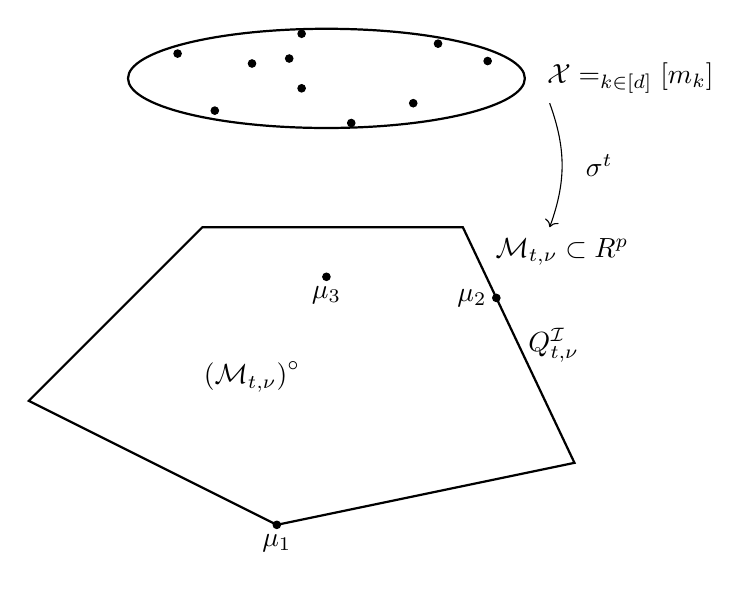
\begin{tikzpicture}[scale=0.315]

    %% States
    \begin{scope}
        [shift={(2,18)}]

        \node[right] at (8.5,0) {$\stateset=\facstates$};

        \draw[thick] (0,0) ellipse (8cm and 2cm);
        \filldraw (-6,1.0) circle (\dotsize);
        \filldraw (-4.5,-1.3) circle (\dotsize);

        \filldraw (-1,1.8) circle (\dotsize);
        \filldraw (1,-1.8) circle (\dotsize);
        \filldraw (3.5,-1.0) circle (\dotsize);
        \filldraw (6.5,0.7) circle (\dotsize);
        \filldraw (4.5,1.4) circle (\dotsize);

        % Base measure support
        \filldraw (-3,0.6) circle (\dotsize);
        \filldraw (-1.5,0.8) circle (\dotsize);
        \filldraw (-1,-0.4) circle (\dotsize);

    \end{scope}

    \draw[->] (11,17) to[bend left=20] (11,12);% node[midway,right] {$\statepolytopemap$};
    \node[anchor=center] at (13,14.5) {$\sstatencoding$};
    \node[anchor=center] at (11.5,11) {$\genmeanset\subset\parspace$};


    \node[below] at (-1,7) {$\sbinteriorof{\genmeanset}$};

    \coordinate (A) at (0,0);

    \node[below] at (A) {$\meanparamof{1}$};
    \draw[fill] (A) circle (\dotsize);

    \coordinate (B) at (12,2.5);

    \coordinate (P2) at (2,10);
    \node[below] at (P2) {$\meanparamof{3}$};
    \draw[fill] (P2) circle (\dotsize);

    \coordinate (C) at (7.5,12);
    \path (B) -- (C) coordinate[pos=0.5] (P4);
    \path (B) -- (C) coordinate[pos=0.7] (P1);
    \node[left] at (P1) {$\meanparamof{2}$};
    \draw[fill] (P1) circle (\dotsize);


    \node[right] at (P4) {$\genfacesetof{\facecondset}$};
    \coordinate (D) at (-3,12);
    \coordinate (E) at (-10,5);

%    \node[below] at ($0.5*(A)+0.5*(E)-(0,1.3)$) {$\genmeanset/\sbinteriorof{\genmeanset}$};

    \draw[thick] (A) -- (B) -- (C) -- (D) -- (E) -- cycle;

\end{tikzpicture}


\end{center}

\subsection{Convex hull}

\begin{lemma}
    For any statistic $\sstat$ and base measure $\basemeasure$, the set of mean parameters is the convex hull of the set
    \begin{align*}
        \genimset = \{\sencsstatat{\indexedshortcatvariables,\selvariable}\wcols\shortcatindices\in\facstates\ncond\basemeasureat{\indexedshortcatvariables}\neq0 \}
    \end{align*}
    that is $\genmeanset = \convhullof{\genimset}$.
\end{lemma}
\begin{proof}
    This follows from
    \begin{align*}
        \bmrealprobof{\basemeasure}
        = \convhullof{
            \frac{1}{\basemeasureat{\indexedshortcatvariables}} \cdot \onehotmapofat{\shortcatindices}{\shortcatvariables}
            \wcols\shortcatindices\in\facstates\ncond\basemeasureat{\indexedshortcatvariables}\neq0} \, .
    \end{align*}
    and for any vertex of this simplex we have
    \begin{align*}
        \contractionof{\frac{1}{\basemeasureat{\indexedshortcatvariables}} \cdot \onehotmapofat{\shortcatindices}{\shortcatvariables},\sencsstatwith,\basemeasurewith}{\selvariable}
        = \sencsstatat{\indexedshortcatvariables,\selvariable} \, .
    \end{align*}
\end{proof}

Thus the polytope of mean parameters depends on the base measure only through its support.

\subsection{Faces}

Let us now continue with the investigation of the faces of the mean parameter polytope. % which we define analogously to Def.~2.1 in \cite{ziegler_lectures_2013}. % ! Defined in Ziegler directly with normals

\begin{definition}
    We say that the convex hull of a subset $\genfaceimset\subset\genimset$ is a face of a mean polytope $\genmeanset$, if and only if there is a face normal vector $\canparamofat{\facesymbol}{\selvariable}\in\parspace$ such that
    \begin{align*}
        \genfaceimset = \argmax_{\meanparamwith\in\genimset} \contraction{\meanparamwith,\canparamofat{\facesymbol}{\selvariable}} \, .
    \end{align*}
    We denote the face as $\facesymbol=\convhullof{\genfaceimset}$.
    The set of all faces of the mean polytope $\genmeanset$ is denoted by $\facelatticeof{\genmeanset}$.
\end{definition}

$\facelatticeof{\genmeanset}$ is called a lattice \cite{ziegler_lectures_2013}.

%\subsection{Characterization of the Boundary by Faces}

%,
%\begin{definition}
%    \label{def:meanPolytopeFaces}
%    Given a mean parameter polytope $\genmeanset$ in the half space representation of \theref{the:meanPolytopeHalfspaces}, and any subset $\mathcal{I}\subset[n]$ we say that the set
%    \begin{align*}
%        \facesymbol
%        = \left\{\meanparamwith\in\genmeanset \wcols \forall_{i\in\mathcal{I}} \, \contraction{\meanparamwith,\normalvecofat{i}{\selvariable}}=\normalboundof{i} \right\}
%    \end{align*}
%    is the face to the constraints $\mathcal{I}$.
%\end{definition}
%
%While all inequalities in a half-space representation are satisfied for any element of the polytope, we defined faces by the additional sharp satisfaction of a subset of the half-space inequalities.
%In this way, the faces build the boundary of $\genmeanset$.
%This can be easily verified, since for any vector $\meanparamwith\in\genmeanset$, for which no halfspace inequalities hold sharply, also a neighborhood satisfies the halfspace inequalities.
%If any halfspace inequality holds sharply, in the other case, the vector is a member of the corresponding face.
%
%% Trivial face containing the whole polytope in case of non-minimal statistics
%If $\sstat$ is not minimal with respect to $\basemeasure$, we find a non-vanishing vector $\vectorat{\selvariable}$ and a scalar $\lambda\in\rr$ such that
%\begin{align*}
%    \contractionof{\sencsstatat{\shortcatvariables,\selvariable},\vectorat{\selvariable},\basemeasurewith}{\shortcatvariables} = \lambda\cdot\basemeasurewith \, .
%\end{align*}
%This implies, that any probability distribution $\probwith$ representable with $\basemeasure$ satisfies
%\begin{align*}
%    \contraction{\probwith,\sencsstatat{\shortcatvariables,\selvariable},\vectorat{\selvariable},\basemeasurewith} = \lambda\cdot \contraction{\probwith,\basemeasurewith} = \lambda \, .
%\end{align*}
%Any $\meanparamwith\in\genmeanset$ then satisfies
%\begin{align*}
%    \contraction{\meanparamwith,\vectorat{\selvariable}} = \lambda \, .
%\end{align*}
%Thus, the polytope $\genmeanset$ is contained in an affine linear subspace and has vanishing interior.
%We can further understand this equation as two half-space inequalities
%\begin{align*}
%    \contraction{\meanparamwith,\vectorat{\selvariable}} \leq \lambda \andspace \contraction{\meanparamwith,\vectorat{\selvariable}} \geq \lambda \, ,
%\end{align*}
%which can be integrated into any half-space representation.
%We conclude, that in the case of non-minimal statistics, the whole polytope $\genmeanset$ is a face itself, since it satisfies these half-space inequalities sharply.


%\subsect{Base measures on faces}

%\begin{lemma}
%    \label{lem:faceConvHullPreimage}
%    For each face $\facesymbol$ we have
%    \begin{align*}
%        \facesymbol
%        = \convhullof{\sencsstatat{\indexedshortcatvariables,\selvariable}\wcols\shortcatindices\in(\sstatencoding)^{-1}(\facesymbol)\ncond\basemeasureat{\indexedshortcatvariables}=1} \, .
%    \end{align*}
%\end{lemma}
%\begin{proof}
%    This holds, since each face is the convex hull of the contained vertices (see Proposition~2.2 and 2.3 in \cite{ziegler_lectures_2013}).
%    Since the vertices are contained in the image of the statistic encoding $\sstatencoding$, the vertices contained in $\facesymbol$ are contained in the set
%    \begin{align*}
%        \sencsstatat{\indexedshortcatvariables,\selvariable}\wcols\shortcatindices\in(\sstatencoding)^{-1}(\facesymbol) \, . & \qedhere
%    \end{align*}
%\end{proof}

%\lemref{lem:faceConvHullPreimage} implies in particular, that faces are mean parameter polytopes with respect to refined base measures.
%For reference in later chapters, we define these refined base measures next as face measures.

We notice, that each face itself is a convex polytope.
What is more, we can characterize these as mean parameter polytopes with respect to refined base measures to be defined next.

\begin{definition}
    \label{def:faceMeasure}
    The face measure to the face $\facesymbol$ of $\genmeanset$ is the boolean tensor $\basemeasureofat{\sstat,\facesymbol}{\shortcatvariables}$ with coordinates to $\shortcatindicesin$ by
    \begin{align*}
        \basemeasureofat{\sstat,\facesymbol}{\indexedshortcatvariables}
        = \begin{cases}
              \basemeasureat{\indexedshortcatvariables} & \ifspace \sstatat{\shortcatindices}\in\genfaceimset \\
              0 & \text{else}
        \end{cases} \, .
%        = \indicatorofat{\sstatencodingof{\shortcatindices}\in\facesymbol}{\shortcatvariables} \, .
    \end{align*}
\end{definition}

We now specify the mean parameter polytope to any face using the face measure as a refinement of the base measure.

\begin{lemma}
    \label{lem:faceAsRefinedPolytope}
    For any face $\facesymbol$ of $\genmeanset$ we have
    \begin{align*}
        \facesymbol = \meansetof{\sstat,\basemeasureof{\sstat,\facesymbol}} \, .
    \end{align*}
\end{lemma}
\begin{proof}
    For any $\shortcatindicesin$ we have $\basemeasureofat{\sstat,\facesymbol}{\indexedshortcatvariables}\neq0$ if and only if $\sstatat{\shortcatindices}\in\genfaceimset$ and $\basemeasureat{\indexedshortcatvariables}\neq0$.
    Thus we have
    \begin{align*}
        \facesymbol
        &= \convhullof{\genfaceimset} \\
        &= \convhullof{\sencsstatat{\indexedshortcatvariables,\selvariable} \wcols \sstatat{\shortcatindices}\in\genfaceimset\ncond \basemeasureat{\indexedshortcatvariables}\neq 0} \\
        &= \convhullof{\sencsstatat{\indexedshortcatvariables,\selvariable} \wcols \basemeasureofat{\sstat,\facesymbol}{\indexedshortcatvariables}\neq 0} \\
        &= \meansetof{\sstat,\basemeasureof{\sstat,\facesymbol}} \, . \qedhere
    \end{align*}
\end{proof}

Representability of a distribution with respect to face measures is an equivalent condition for the mean parameter of a distribution to be on a face, as we show next.

\begin{lemma}
    \label{lem:faceMeasureRepCondition} % was \label{the:facePolytopeCharacterization} in the report
    If and only if for a distribution $\probwith\in\bmrealprobof{\basemeasure}$ and a face $\facesymbol$ we have
    \begin{align*}
        \contractionof{\sencsstatwith,\probwith,\basemeasurewith}{\selvariable}\in\facesymbol\, ,
    \end{align*}
    then $\probwith$ is representable with respect to the base measure
    \begin{align*}
        \genfacemeasurewith \, .
    \end{align*}
\end{lemma}
\begin{proof}
    We have
    \begin{align*}
        \meanparamat{\selvariable} = \sum_{\shortcatindices} \probat{\indexedshortcatvariables}\cdot\basemeasureat{\indexedshortcatvariables} \cdot \genstatshortcatencoding \, .
    \end{align*}
    Let now $\canparamofat{\facesymbol}{\selvariable}$ be a face normal to the face $\genfaceset$.
    We then have
    \begin{align*}
        \contraction{\meanparamwith,\canparamofat{\facesymbol}{\selvariable}}
        = \sum_{\shortcatindicesin}
        \probat{\indexedshortcatvariables}\cdot\basemeasureat{\indexedshortcatvariables} \cdot \contraction{\genstatshortcatencoding,\canparamofat{\facesymbol}{\selvariable}} \, .
    \end{align*}

    Now if and only if $\probat{\indexedshortcatvariables}\cdot\basemeasureat{\indexedshortcatvariables}$ is supported only for $\shortcatindices$ with $\sstatat{\shortcatindices}\in\genfaceimset$ we have that
    \begin{align*}
        \contraction{\meanparamwith,\canparamofat{\facesymbol}{\selvariable}}
        = \max_{\meanparamwith\in\genmeanset} \contraction{\meanparamwith,\canparamofat{\facesymbol}{\selvariable}}
    \end{align*}
    which is equal to $\meanparamwith\in\genfaceset$.
    Thus, if and only if $\meanparamwith\in\genfaceset$ then $\probat{\shortcatvariables}$ is only supported at $\shortcatindices$ in the support of $\genfacemeasurewith$.

%    Now, the $\shortcatindices$ with $\genfacemeasureat{\indexedshortcatvariables}=1$ are exactly those, for which the conditions $\facesymbol$ hold straight.
%    If and only if for a $\shortcatindices$ with $\genfacemeasureat{\indexedshortcatvariables}=0$ we have $\probat{\indexedshortcatvariables}>0$, one of the conditions $\facesymbol$ would not hold straight.
%    Thus, if and only if $\probwith$ is representable with respect to $\genfacemeasureat{\shortcatvariables}$, we have $\meanparamat{\selvariable}\in\facesymbol$.
\end{proof}


Let us now investigate tensor network representations of face measures, based on the basis encoding $\bencodingof{\sstat}$ of a statistic.
% Vertices
%Vertices of $\genmeanset$ are faces with single elements, that is $\{\meanparamwith\}$.
%By \lemref{lem:faceConvHullPreimage} there must be $\meanparam$ must lie in the image of $\sstatencoding$, since otherwise $\genmeanset$ would be empty.
%The vertex measure is then
%\begin{align*}
%    \basemeasureofat{\sstat,\facesymbol}{\shortcatvariables}
%    = \contractionof{\bencodingofat{\sstat}{\headvariables,\shortcatvariables},\onehotmapofat{\meanparam}{\headvariables}}{\shortcatvariables}
%\end{align*}
%Here we use that each $\meanparam\in\facesymbol\cap\imageof{\sstatencoding}$ has integer-valued coordinates and denote
%\begin{align*}
%    \onehotmapofat{\meanparam}{\headvariables} = \bigotimes_{\selindexin} \onehotmapofat{\meanparamat{\indexedselvariable}}{\headvariableof{\selindex}} \, .
%\end{align*}

\begin{theorem}[Face measure representation]
    \label{the:faceMeasureCharacterization}
    For any face $\facesymbol$ of $\meanset$ we have
    \begin{align*}
        \genfacemeasureat{\shortcatvariables}
        =\contractionof{\sstatccwith,\kcoreofat{\facesymbol}{\headvariables},\basemeasurewith}{\shortcatvariables}
    \end{align*}
    where
    \begin{align*}
        \kcoreofat{\facesymbol}{\headvariables}
        = \sum_{\meanparam\in\genfaceimset} \onehotmapofat{\meanparam}{\headvariables} \, .
    \end{align*}
\end{theorem}
\begin{proof}
    For any $\meanparam\in\genfaceimset$ the tensor
    \begin{align*}
        \hypercoreofat{\meanparam}{\shortcatvariables}
        = \contractionof{\sstatccwith,\onehotmapofat{\meanparam}{\headvariables}}{\shortcatvariables}
    \end{align*}
    is the indicator of the preimage of $\meanparam$ under $\sstatencoding$.
    Since preimages the elements in $\genfaceimset$ are disjoint, the support of $\hypercoreofat{\meanparam}{\shortcatvariables}$ is disjoint and their sum
    \begin{align*}
        \sum_{\meanparam\in\genfaceimset} \hypercoreofat{\meanparam}{\shortcatvariables}
    \end{align*}
    is the indicator of the preimage of $\facesymbol$ under $\sstatencoding$.
    The face measure obeys thus
    \begin{align*}
        \basemeasureofat{\sstat,\facesymbol}{\shortcatvariables}
        &= \contractionof{\left(
                              \sum_{\meanparam\in\genfaceimset} \hypercoreofat{\meanparam}{\shortcatvariables}
        \right), \basemeasurewith}{\shortcatvariables} \\
        &= \sum_{\meanparam\in\genfaceimset}
        \contractionof{\sstatccwith,\onehotmapofat{\meanparam}{\headvariables},\basemeasurewith}{\shortcatvariables} \\
        & = \contractionof{\sstatccwith,\kcoreofat{\facesymbol}{\headvariables},\basemeasurewith}{\shortcatvariables} \qedhere
    \end{align*}
\end{proof}

%% Going beyond the report

%%  OLD: restriction to CP
%\begin{definition}
%    The $\cpformat$ rank of a face is
%    \begin{align*}
%        \cprankof{\genfaceset}
%        = \min_{
%            \arbset \wcols \arbset\cap\genimset = \genfaceimset
%            %\{\shortheadindices \wcols \onehotmapof{\shortheadindices}\in\genfaceset\}\subset \arbset \subset \onehotmap(\bigtimes_{\selindexin}[\headdimof{\selindex}]) \ncond
%            %\arbset \cup \{\shortheadindices \wcols \onehotmapof{\shortheadindices}\in\genmeanset/\genfaceset\} = \varnothing
%        }
%        \cprankof{\sum_{v \in \arbset} \onehotmapofat{\imelement}{\headvariables}} \, .
%    \end{align*}
%    By replacing $\cprankof{\cdot}$ with $\bascprankof{\cdot}$ and $\baspluscprankof{\cdot}$ we further define the basis and basis+ CP rank of a face.
%\end{definition}
%
%
%
%The face measures are contraction of the vertex subset encodings with the computation.
%They are \ComputationActivationNetworks{}, when choosing the $\cpformat$ graph with rank at least $\baspluscprankof{\genfaceset}$.
%
%\begin{lemma}
%    For each face of the mean polytope we have
%    \begin{align*}
%        \genfacemeasureat{\shortcatvariables|\varnothing} \in \realizabledistsof{\sstat,\cpformat^{\cprankof{\genfaceset}}} \, ,
%    \end{align*}
%    where $\cpformat^{\cprankof{\genfaceset}}$ is the CP graph with a hidden variable of dimension $\cprankof{\genfaceset}$.
%\end{lemma}
%\begin{proof}
%    We find by definition a set $\arbset$ of basis vectors containing the vertices of the face $\genfacemeasure$ but no further vertices, which has a bas+ $\cpformat$ rank of $\baspluscprankof{\genfaceset}$.
%    We have therefore, that $\normalizationof{\sstatccwith,\onehotmapofat{\arbset}{\headvariables}}{\shortcatvariables}$ is in $\realizabledistsof{\sstat,\cpformat^{\baspluscprankof{\genfaceset}}}$.
%    Further it holds that
%    \begin{align*}
%        \contractionof{\sstatccwith,\onehotmapofat{\arbset}{\headvariables}}{\shortcatvariables}
%        &= \sum_{\shortheadindices\in\arbset \wcols \onehotmapof{\shortheadindices}\in\genfaceset} \contractionof{\sstatccwith,\onehotmapofat{\shortheadindices}{\headvariables}}{\shortcatvariables} \\
%        & \quad \quad + \sum_{\shortheadindices\in\arbset \wcols \onehotmapof{\shortheadindices}\notin\genfaceset} \contractionof{\sstatccwith,\onehotmapofat{\imelement}{\headvariables}}{\shortcatvariables} \\
%        &= \sum_{\shortheadindices\in\arbset \wcols \onehotmapof{\shortheadindices}\in\genfaceset} \contractionof{\sstatccwith,\onehotmapofat{\shortheadindices}{\headvariables}}{\shortcatvariables} \\
%        &= \genfacemeasureat{\shortcatvariables} \, .
%    \end{align*}
%    Here we used, that for $\shortheadindices\in\arbset$ with $\onehotmapof{\shortheadindices}\notin\genfaceset$ is not in the image of $\sstat$ and therefore the contraction of its one-hot encoding with the computation cores vanishes.
%    Thus, $\normalizationof{\sstatccwith,\onehotmapofat{\arbset}{\headvariables}}{\shortcatvariables}$ coincides with the normalized face measure, which is therefore in $\realizabledistsof{\sstat,\cpformat^{\baspluscprankof{\genfaceset}}}$.
%\end{proof}

We now investigate the representation of face measures by \ComputationActivationNetworks{}.

\begin{definition}
    \label{def:faceRepresentability}
    Let $\graph$ be a hypergraph which nodes include $[\seldim]$.
    We say that a face $\genfaceset$ is representable by $\graph$ if and only if there is a set $\arbset$ of basis vectors with
    \begin{align*}
        \arbset \wcols \arbset\cap\genimset = \genfaceimset
    \end{align*}
    and there is a tensor network $\extnet$ with respect to the hypergraph $\graph$ such that
    \begin{align*}
        \contractionof{\extnet}{\headvariables} = \sum_{\imelement\in\arbset} \onehotmapofat{\imelement}{\headvariables} \, . % Can allow for arbitrary weights of the non-supported coordinates!
    \end{align*}
    We call any such tensor network a face activating tensor network.
\end{definition}

\begin{lemma}
    \label{}
    If any only if a face is representable by a hypergraph $\graph$ we have
    \begin{align*}
        \genfacemeasureat{\shortcatvariables|\varnothing} \in \realizabledistsof{\sstat,\graph,\basemeasure} \, .
    \end{align*}
\end{lemma}
\begin{proof}
    For any $\arbset$ with $\arbset \wcols \arbset\cap\genimset = \genfaceimset$ and tensor network $\extnet$ respecting the assumptions of \defref{def:faceRepresentability} we have
    \begin{align*}
        \contractionof{\contractionof{\extnet}{\headvariables},\bencsstatwith}{\shortcatvariables}
        &= \contractionof{\sum_{\imelement\in\arbset}\onehotmapofat{\imelement}{\headvariables},\bencsstatwith}{\shortcatvariables} \\
        &= \contractionof{\sum_{\imelement\in\genfaceimset}\onehotmapofat{\imelement}{\headvariables},\bencsstatwith}{\shortcatvariables} \, .
    \end{align*}
    Here we used in the second equation that only the vertices in $\genimset $ are in the image of $\sstat$.
    It follows, that
    \begin{align*}
        \genfacemeasureat{\shortcatvariables|\varnothing} = \normalizationof{\contractionof{\extnet}{\headvariables},\bencsstatwith,\basemeasurewith}{\shortcatvariables}
    \end{align*}
    and thus $\genfacemeasureat{\shortcatvariables|\varnothing} \in \realizabledistsof{\sstat,\graph,\basemeasure}$.
\end{proof}

Let us now investigate, which normalized face measures can be computed using $\sstat$ and a hypergraph $\graph$.

\begin{example}[Vertices]
    \label{exa:vertexMeasures}
    Vertices $\genfaceset$ are proper faces of affine dimension $0$, that is they consist in single vectors.
    Since all vertices are in the image $\sstatencodingat{\stateset}$, there exists an index tuple $\shortcatindices\in\stateset$ such that $\basemeasureat{\indexedshortcatvariables}=1$ and
    \begin{align*}
        \genfaceset = \{\sencsstatat{\indexedshortcatvariables,\selvariable}\} \, .
    \end{align*}
    Then $\kcoreofat{\facesymbol}{\headvariables}$ is the one-hot encoding of the by an interpretation map $\indexinterpretation$ assigned index to $\sencsstatat{\indexedshortcatvariables,\selvariable}$, that is
    \begin{align*}
        \kcoreofat{\facesymbol}{\headvariables} = \onehotmapofat{\invindexinterpretationat{\sencsstatat{\indexedshortcatvariables,\selvariable}}}{\headvariables} \, .
    \end{align*}
    In particular, the activation core is elementary and the face measure to any vertex is in $\realizabledistsof{\sstat,\elgraph,\basemeasure}$.
\end{example}

While vertices are the minimal non-vanishing faces in the face-lattice (see \cite{ziegler_lectures_2013}), we now show that also the maximal face, namely the polytope itself, is representable with respect to the elementary hypergraph $\elgraph$.

\begin{example}[Maximal face]
    \label{exa:maximalFaceMeasure}
    The maximal face $\genfacesetof{\varnothing}=\genmeanset$ coincides with the mean polytope itself and is given by the choice $\canparamofat{\varnothing}{\selvariable}=\zerosat{\selvariable}$.
    In this case the corresponding activation tensor to the face measure is trivial, that is
    \begin{align*}
        \kcoreofat{\varnothing}{\headvariables} = \onesat{\headvariables} \, .
    \end{align*}
    $\kcoreof{\varnothing}$ is elementary and the normalized face measure $\basemeasureof{\sstat,\varnothing}$ to the maximal face is in $\realizabledistsof{\sstat,\elgraph}$.
\end{example}


Extending \exaref{exa:vertexMeasures}, we can provide a coarse estimation of the hypergraph $\graph$ required to decompose $\kcoreof{\facesymbol}$ for generic faces $\genfaceset$.

\begin{lemma}
    \label{lem:CPfaceRepresentationBound} % Sharpened bound
    Any face $\genfaceset$ is representable by a $\cpformat$ graph with hidden rank
    \begin{align*}
        r = \min\left(\cardof{\genfaceimset},\cardof{\genimset}-\cardof{\genfaceimset}+1\right) \, .
    \end{align*}
\end{lemma}
\begin{proof}
    We show the claim by constructing two face activating tensor networks to $\genfaceset$ in a $\cpformat$ hypergraph with hidden rank $\cardof{\genfaceimset}$ and in a $\cpformat$ hypergraph with hidden rank $\cardof{\genimset}-\cardof{\genfaceimset}+1$.
    To show the first representation we enumerate the vertices by a variable $\decvariable$ with dimension $r=\cardof{\genfaceimset}$, i.e. $\genfaceimset = \{v^{\decindex}[\selvariable] \wcols \decindexin\}$.
    Then we define for $\selindexin$ core tensors $\hypercoreofat{\selindex}{\headvariableof{\selindex},\decvariable}$
    \begin{align*}
        \hypercoreofat{\selindex}{\headvariableof{\selindex},\indexeddecvariable} = \onehotmapofat{\imelementofat{\decindex}{\indexedselvariable}}{\headvariableof{\selindex}} \, .
    \end{align*}
    Then we have
    \begin{align*}
        \contractionof{\{\hypercoreofat{\selindex}{\headvariableof{\selindex},\decvariable}\wcols\selindexin\}}{\headvariables}
        =\sum_{\imelement\in\genfaceimset} \onehotmapofat{\imelement}{\headvariables}
    \end{align*}
    and thus have found an activation tensor network in a $\cpformat$ graph with hidden rank $\cardof{\genfaceimset}$ representing the face $\genfaceset$.

    We continue with the second representation, for which we enumerate the set $\genimset/\genfaceimset$ by $v^{\decindex}[\selvariable]$ where $\decindex\in[\cardof{\genimset}-\cardof{\genfaceimset}]$.
    We define variable $\decvariable$ with dimension $r=\cardof{\genimset}-\cardof{\genfaceimset}+1$ and define for $\selindexin$ core tensors
    \begin{align*}
        \hypercoreofat{\selindex}{\headvariableof{\selindex},\indexeddecvariable}
        =
        \begin{cases}
            -\onehotmapofat{\imelementofat{\decindex}{\indexedselvariable}}{\headvariableof{\selindex}} & \ifspace \decindex < \cardof{\genimset}-\cardof{\genfaceimset} \\
            \onesat{\headvariableof{\selindex}} & \ifspace \decindex = \cardof{\genimset}-\cardof{\genfaceimset}
        \end{cases} \, .
    \end{align*}
    We then have
    \begin{align*}
        \contractionof{\{\hypercoreofat{\selindex}{\headvariableof{\selindex},\decvariable}\wcols\selindexin\}}{\headvariables}
        &=\onesat{\headvariables} - \sum_{\imelement\in\genimset/\genfaceimset} \onehotmapofat{\imelement}{\headvariables} \\
        &= \sum_{\imelement\in\genfaceimset} \onehotmapofat{\imelement}{\headvariables}
        + \sum_{\imelement\in\left(\bigtimes_{\selindexin}[\seldimof{\selindex}]\right)/\genimset} \onehotmapofat{\imelement}{\headvariables} \, .
    \end{align*}
    We have thus found a face activating tensor network for $\genfaceset$ in a $\cpformat$ format with hidden rank $r=\cardof{\genimset}-\cardof{\genfaceimset}+1$.
\end{proof}

\subsection{Partition into Relative Interiors of Faces}

Let us now introduce relative interiors, which enables us to find disjoint partitions of the mean polytope.

\begin{definition}[Relative Interior]
    \label{def:relativeInterior}
    Let $\arbset\subset\parspace$ be an arbitrary set and $\mathcal{L}$ be the affine hull of $\arbset$.
    Then the relative interior, denoted $\sbinteriorof{\arbset}$ is the interior of $\arbset$ in the affine subspace $\mathcal{L}$.
\end{definition}

\begin{lemma}
    \label{lem:relativeInteriorPolytopePartition}
    Any polytope is a disjoint union of the relative interiors of its faces, that is
    \begin{align*}
        \genmeanset = \bigcup_{\facein}^{\cdot} \sbinteriorof{\genfaceset} \, .
    \end{align*}
\end{lemma}
\begin{proof}
    For any $\meanparam\in\genmeanset$ we find a face such that $\meanparam\in\genfaceset$.
    If $\meanparam\notin\sbinteriorof{\genfaceset}$, then there is a face $\genfacesetof{\tilde{\facesymbol}}\subset\genfaceset$ of smaller affine dimension such that $\meanparam\in\facesymbol$.
    When continuing this process we reach a face such that $\meanparam\notin\sbinteriorof{\genfaceset}$, since the faces with affine dimension $0$ are vertices and they coincide with their relative interior because they contain a single vector.
\end{proof}

\begin{definition}
    To each $\meanparam\in\genmeanset$ we denote the unique face $\genfaceset$ with $\meanparam\in\sbinteriorof{\genfaceset}$ by $\facesetofspec{\facesymbol(\meanparam)}{\sstat,\basemeasure}$.
\end{definition}

    \section{Tensor Network Representation of Exponential Families}

We now introduce an architecture of tensor networks, namely \ComputationActivationNetworks{}, and show that exponential families can be represented by them.

\subsection{\ComputationActivationNetworks{}}

Given a statistic $\sstat:\facstates\rightarrow\selstates$ we build its basis encoding tensor
\begin{align*}
    \sstatccwith = \sum_{\shortcatindicesin} \onehotmapofat{\sstat(\shortcatindices)}{\headvariables} \otimes \onehotmapofat{\shortcatindices}{\shortcatvariables} \, .
\end{align*}
A computation network is any representation of $\sstatccwith$ as a tensor network.
These can be constructed in the case statistics being a composition of connective functions.

An activation tensor is $\hypercoreat{\headvariables}$ and the \ComputationActivationNetwork{} of $\sstat$ and $\hypercore$ the tensor
\begin{align*}
    \probwith = \normalizationof{\sstatccwith,\hypercoreat{\headvariables}}{\shortcatvariables} \, .
\end{align*}

We are interested in decomposition formats of $\hypercoreat{\headvariables}$, where we use sets of tensor networks $\tnsetof{\graph}$ on a hypergraph $\graph$.

\begin{definition}
    The family of by $\sstat$ and a $\graph$ computable distributions are
    \begin{align*}
        \realizabledistsof{\sstat,\graph,\basemeasure}
        = \left\{
              \frac{\contractionof{\hypercoreat{\headvariables},\bencsstatwith}{\shortcatvariables}}{\contraction{\hypercoreat{\headvariables},\bencsstatwith,\basemeasurewith}}
              \wcols \hypercoreat{\headvariables} \in \tnsetof{\graph} \right\} \, .
    \end{align*}
\end{definition}

%\subsection{CP decompositions}
%We here introduce the CP decomposition of tensors and the restriction to bas+.
%This will be used to represent face measures as computation activation networks.

\subsection{Exponential Families}

\begin{definition}[Exponential Family]
    \label{def:expFamily}
    Given a statistic function
    \begin{align*}
        \sstat \defcols \facstates \rightarrow \parspace
    \end{align*}
    and a base measure
    \begin{align*}
        \basemeasure \defcols \facstates \rightarrow \rr^+
    \end{align*}
    with $\contraction{\basemeasure}\neq0$, the set $\expfamily=\{\expdist\wcols\canparamwithin\}\subset\bmrealprobof{\basemeasure}$ of probability distributions
    \begin{align*}
        \expdistat{\shortcatvariables}
        = \frac{
            \expof{\contractionof{\sencsstatat{\shortcatvariables,\selvariable},\canparamwith}{\shortcatvariables}}
        }{
            \contraction{\expof{\contractionof{\sencsstatat{\shortcatvariables,\selvariable},\canparamwith}{\shortcatvariables}},\basemeasurewith}
        }
    \end{align*}
    is called the exponential family to $\sstat$.
\end{definition}

To present a tensor network representation, we introduce image interpretation maps
\begin{align*}
    \indexinterpretationof{\selindex} \defcols
    [\cardof{\imageof{\sstatcoordinateof{\selindex}}}] \rightarrow \imageof{\sstatcoordinateof{\selindex}} \, ,
\end{align*}
which enumerate the possible values of each feature.
We treat these maps as tensors with in a variable $\headvariableof{\selindex}$ with values in $[\cardof{\imageof{\sstatcoordinateof{\selindex}}}]$.

\begin{theorem}[Exponential Families are in \ComputationActivationNetworks{}]
    \label{the:expFamilyTensorRep}
    Given any base measure $\basemeasure$ and a sufficient statistic $\sstat$ we enumerate for each coordinate $\selindexin$ the image $\imageof{\sstatcoordinateof{\selindex}}$ by a variable $\headvariableof{\selindex}$ taking values in $[\cardof{\imageof{\sstatcoordinateof{\selindex}}}]$, given an interpretation map
    \begin{align*}
        \indexinterpretationof{\selindex} \defcols
        [\cardof{\imageof{\sstatcoordinateof{\selindex}}}] \rightarrow \imageof{\sstatcoordinateof{\selindex}} \, .
    \end{align*}
    For any canonical parameter vector $\canparamwithin$ we build the activation cores $\softactlegwith$ for each coordinate $\headindexof{\selindex}\in[\cardof{\imageof{\sstatcoordinateof{\selindex}}}]$ by
    \begin{align*}
        \softactleg\left[\indexedheadvariableof{\selindex}\right]
        = \expof{\canparamat{\indexedselvariable} \cdot \indexinterpretationofat{\selindex}{\headindexof{\selindex}} } \,
    \end{align*}
    and have (see \figref{fig:expdistUnaryRealizable})
    \begin{align*}
        \expdistat{\shortcatvariables}
        = \frac{
            \contractionof{\{\bencodingofat{\sstatcoordinateof{\selindex}}{\headvariableof{\selindex},\shortcatvariables} \wcols \selindexin\}\cup\{\softactlegwith \wcols \selindexin\}}{\shortcatvariables}
        }{
            \contraction{\{\bencodingofat{\sstatcoordinateof{\selindex}}{\headvariableof{\selindex},\shortcatvariables} \wcols \selindexin\}\cup\{\softactlegwith \wcols \selindexin\}\cup\{\basemeasurewith\}}
        } \, .
    \end{align*}
\end{theorem}
\begin{proof} %% SHORTENED THE PROOF IN THE REPORT
    For each $\shortcatindicesin$ we have
    \begin{align*}
        &\contractionof{\{\bencodingofat{\sstatcoordinateof{\selindex}}{\headvariableof{\selindex},\shortcatvariables} \wcols \selindexin\}\cup\{\softactlegwith \wcols \selindexin\}}{\indexedshortcatvariables} \\
        &\quad = \prod_{\selindexin} \contraction{\bencodingofat{\sstatcoordinateof{\selindex}}{\headvariableof{\selindex},\indexedshortcatvariables},\softactlegwith} \\
        &\quad = \prod_{\selindexin} \expof{\canparamat{\indexedselvariable}\cdot\indexinterpretationofat{\selindex}{\sstatcoordinateofat{\selindex}{\shortcatindices}}} \\
        &\quad = \expof{\sum_{\selindexin}\canparamat{\indexedselvariable}\cdot\indexinterpretationofat{\selindex}{\sstatcoordinateofat{\selindex}{\shortcatindices}}} \\
        &\quad = \expof{\contractionof{\sencsstatat{\shortcatvariables,\selvariable},\canparamwith}{\indexedshortcatvariables}} \, .
    \end{align*}
    Therefore we have
    \begin{align*}
        \contractionof{\{\bencodingofat{\sstatcoordinateof{\selindex}}{\headvariableof{\selindex},\shortcatvariables} \wcols \selindexin\}\cup\{\softactlegwith \wcols \selindexin\}}{\shortcatvariables}
        = \expof{\contractionof{\sencsstatat{\shortcatvariables,\selvariable},\canparamwith}{\shortcatvariables}} \, .
    \end{align*}
    The claim follows, since this implies that also the contraction of both sides with $\basemeasurewith$ is equivalent.
\end{proof}

\begin{figure}[t]
    \begin{center}
        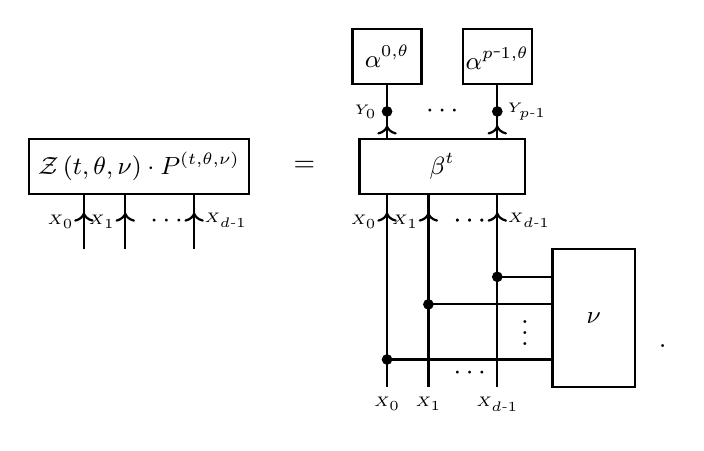
\begin{tikzpicture}[scale=0.35,thick,xscale=1] % , baseline = -3.5pt

    \begin{scope}
        [shift={(-11,0)}]
        \draw (-2,-1) rectangle (6,-3);
        \node[anchor=center] (text) at (2,-2) {\corelabelsize $\partitionfunctionof{\sstat,\canparam,\basemeasure} \cdot \expdist$};
        \draw[-<-] (0,-3)--(0,-5) node[midway,left] {\colorlabelsize $\catvariableof{0}$};
        \draw[-<-] (1.5,-3)--(1.5,-5) node[midway,left] {\colorlabelsize $\catvariableof{1}$};
        \node[anchor=center] (text) at (3,-4) {$\cdots$};
        \draw[-<-] (4,-3)--(4,-5) node[midway,right] {\colorlabelsize $\catvariableof{\atomorder\shortminus1}$};

        \node[anchor=center] (text) at (8,-2) {${=}$};
    \end{scope}

    \draw (-1.25,1) rectangle (1.25,3);
    \node[anchor=center] (text) at (0,2) {\corelabelsize $\softactsymbolof{0,\canparam}$};

    \draw (2.75,1) rectangle (5.25,3);
    \node[anchor=center] (text) at (4,2) {\corelabelsize $\softactsymbolof{\seldim\shortminus 1,\canparam}$};

    \draw[->-] (0,-1)--(0,0);
    \node[left] (text) at (0,0) {\colorlabelsize $\headvariableof{0}$};
    \draw[] (0,0)--(0,1);
    \drawvariabledot{0}{0}
    \node[anchor=center] (text) at (2,0) {$\cdots$};

    \draw[->-] (4,-1)--(4,0);
    \node[right] (text) at (4,0) {\colorlabelsize $\headvariableof{\seccatorder\shortminus1}$};
    \draw[] (4,0)--(4,1);
    \drawvariabledot{4}{0}

    \draw (-1,-1) rectangle (5,-3);
    \node[anchor=center] (text) at (2,-2) {\corelabelsize $\bencodingof{\sstat}$};
    \draw[-<-] (0,-3)--(0,-5) node[midway,left] {\colorlabelsize $\catvariableof{0}$};
    \draw[-<-] (1.5,-3)--(1.5,-5) node[midway,left] {\colorlabelsize $\catvariableof{1}$};
    \node[anchor=center] (text) at (3,-4) {$\cdots$};
    \draw[-<-] (4,-3)--(4,-5) node[midway,right] {\colorlabelsize $\catvariableof{\atomorder\shortminus1}$};


    \begin{scope}
        [shift={(0,-4)}]
        \draw[] (0,1)--(0,-6);
        \node[below] (text) at (0,-6) {\colorlabelsize $\catvariableof{0}$};
        \drawvariabledot{0}{-5}
        \draw[] (1.5,1)--(1.5,-6);
        \node[below] (text) at (1.5,-6) {\colorlabelsize $\catvariableof{1}$};
        \drawvariabledot{1.5}{-3}
        \node[anchor=center] (text) at (3,0) {$\cdots$};
        \node[anchor=center] (text) at (3,-5.5) {$\cdots$};
        \draw[] (4,1)--(4,-6);
        \node[below] (text) at (4,-6) {\colorlabelsize $\catvariableof{\atomorder\shortminus1}$};
        \drawvariabledot{4}{-2}

        \draw[] (0,-5) -- (6,-5);
        \draw[] (1.5,-3) -- (6,-3);
        \node[anchor=center] (text) at (5,-3.75) {$\vdots$};
        \draw[] (4,-2) -- (6,-2);
        \draw (6,-1) rectangle (9, -6);
        \node[anchor=center] (text) at (7.5,-3.5) {\corelabelsize $\basemeasure$};

        \node[anchor=center] (text) at (10,-4.5) {$.$};

    \end{scope}

\end{tikzpicture}
    \end{center}
    \caption{Representation of a member in an exponential family by a \ComputationActivationNetwork{} with elementary activation.
    Since the right hand side is not normalized both sides are equal up to a constant.}\label{fig:expdistUnaryRealizable}
\end{figure}

We will use the following well known property (see e.g. \cite{brown_fundamentals_1987}), that there is a one-to-one map between the canonical parameters and the mean parameters.

\begin{lemma}
    \label{lem:interiorRepExpFamily}
    The set of mean parameters of the members of an exponential family is the relative interior of the mean polytope.
    For $\canparam,\seccanparam\in\parspace$ with
    \begin{align*}
        \uniquantwrtof{\selindexin}{
            \contraction{\expdistofat{\sstat,\canparam,\basemeasure}{\shortcatvariables},\sstatcoordinateofat{\selindex}{\shortcatvariables},\basemeasurewith}
            = \contraction{\expdistofat{\sstat,\seccanparam,\basemeasure}{\shortcatvariables},\sstatcoordinateofat{\selindex}{\shortcatvariables},\basemeasurewith}
        }
    \end{align*}
    we furthermore have $\expdistofat{\sstat,\canparam,\basemeasure}{\shortcatvariables}=\expdistofat{\sstat,\seccanparam,\basemeasure}{\shortcatvariables}$.
\end{lemma}
\begin{proof}
    See The~3.3 in \cite{wainwright_graphical_2008}.
\end{proof}

Based on this property we define the forward and backward mappings to an exponential family.

\begin{definition}
    The forward map of an exponential family is the map
    \begin{align*}
        \forwardmap  \defcols \parspace \rightarrow \sbinteriorof{\genmeanset}
    \end{align*}
    defined as
    \begin{align*}
        \uniquantwrtof{\selindexin}{
            \forwardmapofat{\canparam}{\indexedselvariable}
            = \contraction{\expdistofat{\sstat,\canparam,\basemeasure}{\shortcatvariables},\sstatcoordinateofat{\selindex}{\shortcatvariables},\basemeasurewith}
        }
    \end{align*}
    Any map $\backwardmap: \sbinteriorof{\genmeanset}\rightarrow \parspace$ with $\backwardmap\circ\forwardmap=\mathrm{Id}$ is called a backward map.
\end{definition}

    \section{Main results: Tensor network representation of maximum entropy distributions}

Given the mean polytope discussion we now characterize the tensor network representation of maximum entropy distributions.



\subsection{Maximum entropy on the interior}

A classical result states, that the maximum entropy distribution is in the exponential family $\expfamilyof{\sstat,\basemeasure}$ (see e.g. \cite{koller_probabilistic_2009}).

\begin{theorem}
    \label{the:maxEntropyInterior}
    %If the only face $\genfacesetof{\facecondset}$ of $\genmeanset$ with $\meanparam\in\genfacesetof{\facecondset}$ is $\genmeanset$ itself
    If and only if $\genmean$ is in the relative interior of $\genmeanset$, then the unique solution of the maximum entropy problem is the distribution
    \begin{align*}
        \expdistofat{\sstat,\genmean,\basemeasure}{\shortcatvariables}\in\expfamilyof{\sstat,\basemeasure}
    \end{align*}
    with $\contractionof{\expdistofat{\sstat,\genmean,\basemeasure}{\shortcatvariables},\sencsstatwith}{\selvariable}=\genmeanat{\selvariable}$.
\end{theorem}
\begin{proof}
    By \lemref{lem:interiorRepExpFamily}
    \begin{align*}
        \meanparamwith \in \sbinteriorof{\genmeanset}  \, ,
    \end{align*}
    there is a canonical parameter $\canparam$ with
    \begin{align*}
        \contractionof{\expdistofat{\sstat,\canparam,\basemeasure}{\shortcatvariables},\sencsstatwith,\basemeasurewith}{\selvariable}=\meanparamat{\selvariable} \, .
    \end{align*}

    For any other feasible distribution $\secprobat{\shortcatvariables}$ we also have $\contractionof{\secprobat{\shortcatvariables},\sencsstatwith,\basemeasurewith}{\selvariable}=\meanparamat{\selvariable}$ and thus
    \begin{align*}
        \centropyofwrt{\secprobtensor}{\expdistof{(\sstat,\canparam,\basemeasure)}}{\basemeasure}
        &= -\contraction{\secprobtensor,\lnof{\expdistofat{(\sstat,\canparam,\basemeasure)}{\shortcatvariables}},\basemeasurewith} \\
        &= -\contraction{\secprobtensor,\sencsstatwith,\canparamwith,\basemeasurewith} + \cumfunctionof{\canparam} \\
        &= - \contraction{\canparamwith,\meanparamwith} + \cumfunctionof{\canparam} \\
        &= \sentropyofwrt{\expdistof{(\sstat,\canparam,\basemeasure)}}{\basemeasure} \, .
    \end{align*}
    With the Gibbs inequality we have if $\secprobtensor\neq\expdistof{(\sstat,\canparam,\basemeasure)}$
    \begin{align*}
        \sentropyofwrt{\expdistof{(\sstat,\estcanparam,\basemeasure)}}{\basemeasure}  - \sentropyofwrt{\secprobtensor}{\basemeasure}
        = \centropyofwrt{\secprobtensor}{\expdistof{(\sstat,\estcanparam,\basemeasure)}}{\basemeasure}  - \sentropyofwrt{\secprobtensor}{\basemeasure}  > 0 \,
    \end{align*}
    and thus $\sentropyofwrt{\secprobtensor}{\basemeasure}<\sentropyofwrt{\secprobtensor}{\basemeasure}$.
    Therefore, if $\secprobtensor$ does not coincide with $\expdistof{(\sstat,\estcanparam,\basemeasure)}$, it is not a maximum entropy distribution.
\end{proof}

%Exponential families are in $\elrealizabledistsof{\sstat}$, if and only if $\normalizationof{\basemeasure}{\shortcatvariables}\in\elrealizabledistsof{\sstat}$.
%If $\normalizationof{\basemeasure}{\shortcatvariables}\in\elrealizabledistsof{\sstat}$ and $\meanparamwith \in \sbinteriorof{\genmeanset} $ we therefore have a sparse representation of the maximum entropy distribution with elementary activation tensors.

\subsection{Main result}

Our main result generalizes the maximum entropy characterization of \theref{the:maxEntropyInterior} to arbitrary mean parameters.

\begin{theorem}[Generic characterization of Maximum Entropy Solutions]
    \label{the:MAINgenMaxEntChar}
    Let $\sstat$ be a statistic and $\basemeasure$ a base measure.
    For any $\meanparamwith$ the maximum entropy problem has a feasible distribution, if and only if $\meanparamwith\in\genmeanset$.
    In case $\meanparamwith\in\genmeanset$ denote the unique face of $\genmeanset$ with $\meanparam$ in its relative interior by $\genfaceset$ (see \defref{def:relativeInterior}).
    Then the solution of the maximum entropy problem is the member
    \begin{align*}
        \expdistof{(\sstat,\backwardmapwrtof{\sstat,\genfacemeasure}{\meanparam},\genfacemeasure)}
    \end{align*}
    of the exponential family $\expfamilyof{\sstat,\genfacemeasure}$, where $\genfacemeasure$ is the face measure (see \defref{def:faceMeasure}).
    If for a hypergraph $\graph$, which nodes appear all in at least one edge, the face is representable with respect to $\graph$ (see \defref{def:faceRepresentability}), then the maximum entropy distribution is in $\realizabledistsof{\sstat,\graph,\basemeasure}$.
    %$\genfacemeasure\in\$ is an elementary \ComputationActivationNetwork{}, then $\expdistof{(\sstat,\backwardmapwrtof{\sstat,\genfacemeasure}{\meanparam},\genfacemeasure)}$ is a \ComputationActivationNetwork{} with respect to the CP graph of rank $\cprankof{\genfaceset}$.
\end{theorem}

Note, that while we use refined base measures $\genfacemeasure$ to characterize the maximum entropy distribution, \theref{the:MAINgenMaxEntChar} states a representation with respect to the original base measure $\basemeasure$.

To prepare for the proof of this theorem we first show in an auxiliary lemma that we can reduce the set of feasible distributions in \probref{prob:maxEntropy}.

\begin{lemma}
    \label{lem:maxEntReduction}
    For any $\meanparamwith\in\genmeanset$ and a face $\genfaceset$ with $\meanparamwith\in\sbinteriorof{\genfaceset}$ we have that the solutions of $\mathrm{P}_{\sstat,\meanparam,\basemeasure}$ and $\mathrm{P}_{\sstat,\meanparam,\genfacemeasure}$ coincide.
\end{lemma}
\begin{proof}
    By \lemref{lem:faceMeasureRepCondition} all feasible distributions are representable by the with the face measure refined base measure.
    We have that any for $\mathrm{P}_{\sstat,\meanparam,\basemeasure}$ feasible distribution $\probwith$ satisfies
    \begin{align*}
        \contraction{\probwith,\genfacemeasure} = 1 \,
    \end{align*}
    and thus $\probwith\in\realizabledistsof{\sstat,\genfacemeasure}$.
    Conversely, any $\probwith\in\realizabledistsof{\sstat,\genfacemeasure}$ satisfies
    \begin{align*}
        \contraction{\probwith,\genfacemeasure} = \contraction{\probwith,\basemeasure} = 1
    \end{align*}
    and thus $\probwith\in\realizabledistsof{\sstat,\basemeasure}$.
    Problem $\mathrm{P}_{\sstat,\meanparam,\basemeasure}$ is thus equal to
    \begin{align*}
        \argmax_{\probwith\in\realizabledistsof{\sstat,\genfacemeasure}} \sentropyofwrt{\probwith}{\basemeasure}
        \stspace
        \forall_{\selindexin} \wcols
        \contractionof{\probwith,\sstatcoordinateofat{\selindex}{\shortcatvariables},\basemeasurewith}{\selvariable} = \genmeanat{\indexedselvariable}
    \end{align*}
    We further have that any $\probwith\in\realizabledistsof{\sstat,\genfacemeasure}$
    \begin{align*}
        \sentropyofwrt{\probwith}{\basemeasure} = \sentropyofwrt{\probwith}{\genfacemeasure}
    \end{align*}
    and arrive together with the above equivalence at the claim.
\end{proof}


\begin{proof}[Proof of \theref{the:MAINgenMaxEntChar}]
    \textbf{Feasibility Claim:}
    If and only if $\meanparamwith\in\genmeanset$ then there is by definition a by $\basemeasure$ representable $\probwith$ reproducing $\meanparamwith$.
    Thus if and only if $\meanparamwith\in\genmeanset$ there is a feasible distribution for the maximum entropy problem. \\

    \textbf{Characterization Claim:}
    We use the following argumentation to show the second claim:
    \begin{itemize}
        \item By \lemref{lem:relativeInteriorPolytopePartition} for any $\meanparam$ we find a unique face $\genfaceset$.
        \item By \lemref{lem:maxEntReduction} we can reduce the maximum entropy problem \probref{prob:maxEntropy} to $\mathrm{P}_{\sstat,\meanparam,\genfacemeasure}$ to the base measure $\genfacemeasure$.
        \item By \lemref{lem:faceAsRefinedPolytope} the face $\genfaceset$ coincides with the polytope $\meansetof{\sstat,\genfacemeasure}$ and in particular $\meanparam$ is in the relative interior of that polytope.
        \item We can now apply \theref{the:maxEntropyInterior} and get a characterization of the maximum entropy solution as a member of the exponential family.
    \end{itemize}

    \textbf{Representation Claim:} % ! WE DO A CHANGE OF BASE MEASURE HERE
    By \defref{def:faceRepresentability} we find a tensor network $\extnet$ on $\graph$ representing the face measure, that is
    \begin{align*}
        \genfacemeasurewith = \contractionof{\{\extnet\}\cup\{\bencsstatwith,\basemeasurewith\}}{\shortcatvariables} \, .
    \end{align*}
    We now contract the activation vectors of the exponential family on this tensor network (see \figref{fig:maxEntropyActcore}).
    To this end we choose a hyperedge $\edge(\selindex)$ to each node $\selindexin$, which is possible by assumption, and define a tensor network $\tilde{\tnet}^{\graph}$ by core tensors
    \begin{align*}
        \sechypercoreofat{\edge}{\headvariableof{\edge}} = \contractionof{\{\hypercoreofat{\edge}{\headvariableof{\edge}}\}\cup\{\softactlegat{\headvariableof{\selindex}}\wcols\edge=\edge(\selindex)\}}{\edgevariables} \, .
    \end{align*}
    Now we have that
    \begin{align*}
        \contractionof{\{\tilde{\tnet}^{\graph}\}\cup\{\bencsstatwith,\basemeasurewith\}}{\shortcatvariables}
        = \contractionof{\softacttensorat{\headvariables},\bencsstatwith,\genfacemeasurewith}{\shortcatvariables}
    \end{align*}
    Thus, the activation tensor network $\tilde{\tnet}^{\graph}$ represents the maximum entropy distribution $\probof{\sstat,\meanparam,\basemeasure}$ in the family $\realizabledistsof{\sstat,\graph,\basemeasure}$ of \ComputationActivationNetworks{}.
\end{proof}

\begin{figure}[t]
    \begin{center}
        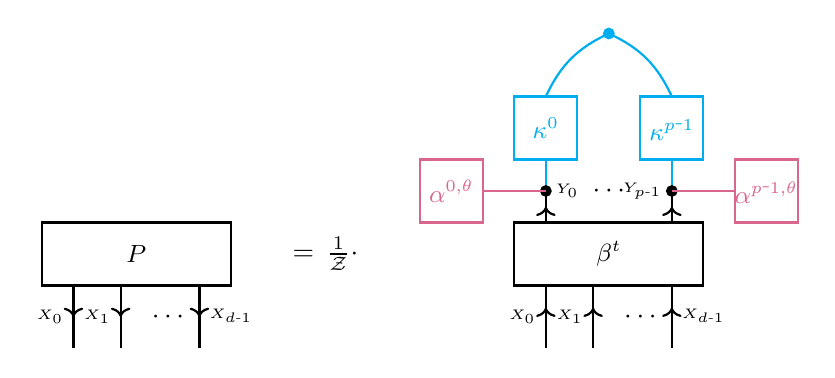
\begin{tikzpicture}[scale=0.4,thick,xscale=1] % , baseline = -3.5pt

    \begin{scope}
        [shift={(-15,0)}]
        \draw (-1,-1) rectangle (5,-3);
        \node[anchor=center] (text) at (2,-2) {\corelabelsize $\probtensor$};
        \draw[->-] (0,-3)--(0,-5) node[midway,left] {\colorlabelsize $\catvariableof{0}$};
        \draw[->-] (1.5,-3)--(1.5,-5) node[midway,left] {\colorlabelsize $\catvariableof{1}$};
        \node[anchor=center] (text) at (3,-4) {$\cdots$};
        \draw[->-] (4,-3)--(4,-5) node[midway,right] {\colorlabelsize $\catvariableof{\atomorder\shortminus1}$};

        \node[anchor=center] (text) at (8,-2) {$= \,\frac{1}{\partitionfunction} \cdot $};
    \end{scope}

    %% Condition cores: Boolean cores selecting faces
    \draw[\concolor] (4,3) to[bend right=20] (2,5);
    \draw[\concolor] (0,3) to[bend left=20] (2,5);
    \draw[fill,\concolor] (2,5) circle (\dotsize);

    \draw[\concolor] (-1,1) rectangle (1,3);
    \node[anchor=center,\concolor] (text) at (0,2) {\corelabelsize $\hardactsymbolof{{0}}$};

    \draw[\concolor] (3,1) rectangle (5,3);
    \node[anchor=center,\concolor] (text) at (4,2) {\corelabelsize $\hardactsymbolof{{\seccatorder\shortminus1}}$};

    \draw[->-] (0,-1)--(0,0);
    \node[right] (text) at (0,0) {\colorlabelsize $\headvariableof{0}$};
    \draw[\concolor] (0,0)--(0,1);
    \drawvariabledot{0}{0}
    \node[anchor=center] (text) at (2,0) {$\cdots$};

    \draw[\probcolor] (0,0) -- (-2,0);
    \draw[\probcolor] (-2,1) rectangle (-4,-1);
    \node[anchor=center,\probcolor] (text) at (-3,0) {\corelabelsize $\softactsymbolof{0,\canparam}$};

    \draw[->-] (4,-1)--(4,0);
    \node[left] (text) at (4,0) {\colorlabelsize $\headvariableof{\seccatorder\shortminus1}$};
    \draw[\concolor] (4,0)--(4,1);
    \drawvariabledot{4}{0}

    \draw[\probcolor] (4,0) -- (6,0);
    \draw[\probcolor] (6,1) rectangle (8,-1);
    \node[anchor=center,\probcolor] (text) at (7,0) {\corelabelsize $\softactsymbolof{\seccatorder\shortminus1,\canparam}$};

    \draw (-1,-1) rectangle (5,-3);
    \node[anchor=center] (text) at (2,-2) {\corelabelsize $\bencodingof{\sstat}$};
    \draw[-<-] (0,-3)--(0,-5) node[midway,left] {\colorlabelsize $\catvariableof{0}$};
    \draw[-<-] (1.5,-3)--(1.5,-5) node[midway,left] {\colorlabelsize $\catvariableof{1}$};
    \node[anchor=center] (text) at (3,-4) {$\cdots$};
    \draw[-<-] (4,-3)--(4,-5) node[midway,right] {\colorlabelsize $\catvariableof{\atomorder\shortminus1}$};


\end{tikzpicture}
    \end{center}
    \caption{
        Tensor network decomposition of maximum entropy distributions to the constraint $\meanparamat{\selvariable}=\contractionof{\probtensor,\sencsstat}{\selvariable}$.
        Blue: Constraint activation cores $\hardactsymbolof{\selindex}$ in a $\cpformat$ decomposition, representing the face measure to the minimal face, such that $\meanparam\in\genfacesetof{\facecondset}$.
        Red: Probabilistic activation cores $\softactlegwith$ in an elementary decomposition, where each leg core is a scaled exponentials evaluated on the enumerated image $\imageof{\sstatcoordinateof{\selindex}}$.
    }\label{fig:maxEntropyActcore}
\end{figure}

\subsection{Family of maximum entropy distributions}

The family of maximum entropy distributions is the set
\begin{align*}
    \{\probof{\sstat,\meanparam,\basemeasure} \wcols \meanparam\in\genmeanset\ncond \probof{\sstat,\meanparam,\basemeasure} \quad\text{is a solution of }\quad \probref{prob:maxEntropy}\} \, .
\end{align*}

By \theref{the:expFamilyTensorRep} this is the union of exponential families to each face measure.
Note that these families are disjoint, since each member of an exponential family has support by the support of the face measure.

    \section{Characterization for boolean statistics}

\red{We here study the face CP ranks in case of boolean statistics.
We further show that any elementary \ComputationActivationNetwork{} to boolean statistics is a maximum entropy distribution.}

For boolean statistics $\hlnstat:\facstates\rightarrow\bigtimes_{\selindexin}[2]$ the mean polytope is a subset of the cube $\fullparcube$.
In this case, any boolean vector in $\meansetof{\hlnstat,\basemeasure}$ is a vertex.
It follows, that any distribution reproducing a mean parameter $\meanparamwith$ on the relative interior of $\meansetof{\hlnstat,\basemeasure}$ is positive with respect to $\basemeasure$.

We apply the exponential distribution characterization of the maximum entropy distribution and get that the maximum entropy distribution is in $\elrealizabledistsof{\sstat}$, if and only if the face measure is in $\elrealizabledistsof{\sstat}$.
This is exactly the case, when the face is an intersection of the mean polytope with a face of the cupe $\fullparcube$.

\subsection{Characterization of elementary representable faces}

We first show in the following example, that all faces of a hypercube are representable by elementary activation tensors.

\begin{example}[Hypercube]
    \label{exa:hypercubeFaces}
    In cases where $\shortcatvariables$ are boolean and we have $\selindexin$ features
    \begin{align*}
        \formulaofat{\selindex}{\indexedshortcatvariables} = \catindexof{\selindex}
    \end{align*}
    the mean polytope is the hypercube
    \begin{align*}
        \meansetof{\{\formulaof{\selindex}\wcols\selindexin\},\trivbm} = \fullparcube \, .
    \end{align*}
    The non-empty faces in the face lattice $\facelatticeof{\fullparcube}$ can be enumerated by subsets $\variableset\subset[\seldim]$ and indices $\headindexof{\variableset}\in\bigtimes_{\selindex\in\variableset}[2]$ and represented by the cartesian products
    \begin{align*}
        % \facesetofspec{(\variableset,\headindexof{\variableset})}{} %{\{\formulaof{\selindex}\wcols\selindexin\},\trivbm}
        \facesymbolof{(\variableset,\headindexof{\variableset})}
        = \bigtimes_{\selindexin} \mathcal{I}^{l,(\variableset,\headindexof{\variableset})}
    \end{align*}
    where
    \begin{align*}
        \mathcal{I}^{l,(\variableset,\headindexof{\variableset})}
        = \begin{cases}
        [0,1]
              & \ifspace \selindex\notin\variableset \\
              \{\headindexof{\selindex}\}& \ifspace \selindex\in\variableset
        \end{cases} \, .
    \end{align*}
    Each of these faces can be represented with respect to the elementary graph $\elgraph$, namely by the tensor product of leg vectors
    \begin{align*}
        %\actcoreofat{\selindex}{\headvariableof{\selindex}}
        \hardactlegwith
        = \begin{cases}
              \onesat{\headvariableof{\selindex}} & \ifspace \selindex\notin\variableset \\
              \onehotmapofat{\headindexof{\selindex}}{\headvariableof{\selindex}}& \ifspace \selindex\in\variableset
        \end{cases} \, .
    \end{align*}
    %\red{This will later be interpreted by propositional logics as the example of atomic formulas.}
\end{example}

Orienting on \exaref{exa:hypercubeFaces} we define cube-likeness of faces and polytopes.

\begin{definition}
    \label{def:cubeLike}
    We say that a face $\facesymbol$ of $\hlnmeanset$ is cube-like, if it is empty or there is $\variableset\subset[\seldim]$ and $\headindexof{\variableset}\in\bigtimes_{\selindex\in\variableset}[2]$ such that
    \begin{align*}
        \facesymbol = \meansetof{\hlnstat,\basemeasure} \cap \facesymbolof{(\variableset,\headindexof{\variableset})} \, .
    \end{align*}
    We further say that a polytope $\hlnmeanset$ is cube-like, if all faces $\facesymbol\in\facelatticeof{\hlnmeanset}$ are cube-like.
\end{definition}

We now show that a face is cube-like if and only if it is representable by an elementary tensor.

\begin{theorem}
    \label{the:faceMeasureHardLogicNetworks}
    Let $\hlnstat$ be a boolean statistic, $\basemeasure$ a base measure and $\facesymbol$ be a face of $\hlnmeanset$.
    Then the following are equivalent:
    \begin{itemize}
        \item[(i)] $\facesymbol$ is cube-like (see \defref{def:cubeLike}).
        \item[(ii)] $\facesymbol$ is representable by an elementary tensor (see \defref{def:faceRepresentability}).
   \end{itemize}
\end{theorem}
\begin{proof}
    If the face is empty, i.e. $\facesymbol=\varnothing$, it is by definition cube-like and has $\zerosat{\headvariables}$ as an elementary activation tensor.
    We therefore assume in the following $\facesymbol\neq\varnothing$.

    (i)$\Rightarrow$(ii):
    Let us assume that $\facesymbol$ is cube-like, that is there is $\variableset\subset[\seldim]$ and $\headindexof{\variableset}\in\bigtimes_{\selindex\in\variableset}[2]$ such that $\facesymbol = \meansetof{\hlnstat,\basemeasure} \cap \facesymbolof{(\variableset,\headindexof{\variableset})}$.
    We use that $\facesymbol,\meansetof{\hlnstat,\basemeasure}$ and $\facesymbolof{(\variableset,\headindexof{\variableset})}$ are the convex hulls of the cube vertex sets $\imsetof{\hlnstat,\meanset}{\facesymbol}$, $\imsetof{\hlnstat,\meanset}{}$ and
    \begin{align}\label{eq:cubeFaceVertices}
        \imsetof{}{(\variableset,\headindexof{\variableset})} = \{\imelementwith \wcols \forall \selindex\in\variableset \imelementat{\indexedselvariable}=\headindexof{\variableset}\} \, ,
    \end{align}
    which implies that
    \begin{align*}
        \imsetof{\hlnstat,\meanset}{\facesymbol} = \imsetof{}{(\variableset,\headindexof{\variableset})} \cap \imsetof{\hlnstat,\meanset}{} \, .
    \end{align*}
    Thus, we can choose $\arbset=\imsetof{\hlnstat,\meanset}{\facesymbol}$ for the representation of the face $\facesymbol$ (see \defref{def:faceRepresentability}) and further have that
    \begin{align*}
        \sum_{\imelementwith\in\imsetof{}{(\variableset,\headindexof{\variableset})}}
        = \bigotimes_{\selindexin} \hardactlegwith \, .
    \end{align*}
    We have thus found an elementary activation tensor for the face $\facesymbol$.

    (ii)$\rightarrow$(i)
    Conversely, let $\acttensorwith$ be an elementary activation tensor of the face $\facesymbol$ in $\hlnmeanset$.
    Since $\acttensorwith$ is the sum of different one-hot encodings it is boolean and we find an elementary decomposition $\acttensorwith=\bigotimes_{\selindexin}\acttensorlegwith$ such that the leg vectors $\acttensorwith$ are boolean.
    Since $\facesymbol\neq\varnothing$ we further have for $\selindexin$ that $\acttensorlegwith\neq\zerosat{\headvariableof{\selindex}}$, and thus $\acttensorlegwith\in \{\fbasisat{\headvariableof{\selindex}},\tbasisat{\headvariableof{\selindex}},\onesat{\headvariableof{\selindex}}\}$
    We construct a set $\variableset\subset[\seldim]$
    \begin{align*}
        \variableset = \left\{\selindex \wcols {\acttensorlegwith}\neq\onesat{\headvariableof{\selindex}}\right\}
    \end{align*}
    and a tuple
    \begin{align*}
        \headindexof{\selindex}
        = \begin{cases}
              1 & \ifspace {\acttensorlegwith}=\onehotmapofat{1}{\headvariableof{\selindex}} \\
              0 & \ifspace {\acttensorlegwith}=\onehotmapofat{0}{\headvariableof{\selindex}}
        \end{cases} \, .
    \end{align*}
    By construction ${\acttensorlegwith} = \hardactlegwith$ (see \exaref{exa:hypercubeFaces}) follows for all $\selindexin$ and therefore $\acttensorwith=\hardacttensorwith$.
    We therefore have for the set \eqref{eq:cubeFaceVertices}
    \begin{align*}
        \acttensorwith = \sum_{\imelement\in\imsetof{}{\variableset,\headindexof{\variableset}}} \onehotmapofat{\imelement}{\headvariables}
    \end{align*}
    and since $\acttensorwith$ is an activation tensor for $\facesymbol$, that 
    \begin{align*}
        \imsetof{\hlnstat,\meanset}{\facesymbol}
        = \imsetof{}{\variableset,\headindexof{\variableset}}\cap\imsetof{\hlnstat,\meanset}{} \, .
    \end{align*}
    Taking convex hulls on both sides, this is equivalent to
    \begin{align*}
        \facesymbol = \facesymbolof{(\variableset,\headindexof{\variableset})} \cap \meansetof{\hlnstat,\basemeasure} \, .
    \end{align*}
    We conclude that $\facesymbol$ is cube-like.
\end{proof}

Let us now give with the standard simplices a class of convex polytopes, which are not hypercubes, but cube-like.

\begin{example}[Simplices are cube-like]
    The $(\seldim-1)$-dimensional standard simplex $\meansetof{\triangle,\seldim-1}$ in $[0,1]^{\seldim}$ is the convex hull of the vertex sets
    \begin{align*}
        \imset = \{\onehotmapofat{\selindex}{\selvariable} \wcols\selindexin\} \, . % selvariable
    \end{align*}
    %where $\selvariable$ takes values in $[\seldim-1]$.
    The simplex is the mean polytope of the $\seldim$-dimensional statistic with
    \begin{align*}
        \sstatcoordinateof{\selindex} \defcols [\seldim] \rightarrow [2] \quad, \quad
        \sstatcoordinateofat{\selindex}{\secselindex}
        = \begin{cases}
              1 & \ifspace \secselindex = \selindex \\
              0 & \ifspace \secselindex \neq \selindex
        \end{cases} \, .
    \end{align*}
    This is sometimes referred to as the probability simplex, since it represents all distributions of a discrete variable with $\seldim$ states.

    The face lattice of the simplex consists is enumerated by subsets of $[\seldim]$ as
    \begin{align*}
        \facelatticeof{\meansetof{\triangle,\seldim-1}}
        = \{\facesymbolof{\variableset}\wcols\variableset\subset[\seldim]\}
    \end{align*}
    where the faces are
    \begin{align*}
        \facesymbolof{\variableset} = \convhullof{\onehotmapofat{\selindex}\wcols\selindex\in\variableset}
    \end{align*}
    and therefore itself $(\cardof{\variableset}-1)$-dimensional standard simplices.
    The partial order of the faces coincides with the inclusion order of subsets $\variableset$.
    Furthermore, each face $\facesymbolof{\variableset}$ is cube-like since
    \begin{align*}
        \facesymbolof{\variableset} = \meansetof{\triangle,\seldim-1} \cap \facesymbolof{[\seldim]/\variableset,0_{[\seldim]/\variableset}}
    \end{align*}
    where $\facesymbolof{[\seldim]/\variableset,0_{[\seldim]/\variableset}}$ are faces of the hypercube following the notation of \exaref{exa:hypercubeFaces}.
\end{example}

\subsection{Set of maximum entropy distributions}

\begin{theorem}
    Any distribution in $\realizabledistsof{\hlnstat,\elgraph,\basemeasure}$ is a maximum entropy distribution with respect to $(\hlnstat,\meanparam,\basemeasure)$ where $\meanparam$ is its mean parameter.
    Any maximum entropy distribution is realized by $\realizabledistsof{\hlnstat,\elgraph,\basemeasure}$ if and only if the mean parameter is in the relative interior of a cube-like face.
\end{theorem}
\begin{proof}
    First claim by decomposing any elementary tensor into exponential and hard activation core.
    Second claim by characterization of elementary faces by cube-likeness.
\end{proof}

We can now use the same notation as applied for hypercubes to classify the faces of a cube-like polytope.

\subsection{Interpretation by propositional formulas}

We can understand each feature as a propositional formula and the variables $\shortcatvariables$ as atoms (possibly after a binarization).

Each vertex of the cube, which is not a vertex of the polytope corresponds with the unsatisfiability of a formula
\begin{align*}
    \bigwedge_{\selindexin} \lnot^{1-\meanparamat{\indexedselvariable}} \formulaofat{\selindex}{\shortcatvariables}
\end{align*}
which is equal with any of the entailment statements for $\variableset\subset[\seldim]$ % Can extend to any partition!
\begin{align*}
    \left(\bigwedge_{\selindex\in\variableset} \lnot^{1-\meanparamat{\indexedselvariable}} \formulaofat{\selindex}{\shortcatvariables} \right)
    \models \left(\bigwedge_{\selindex\in\variableset}\lnot^{\meanparamat{\indexedselvariable}} \formulaofat{\selindex}{\shortcatvariables} \right) \, .
\end{align*}

Along this interpretation we can easily construct examples of statistics, which polytopes are not cube-like.

\begin{example}[Maximum entropy distribution with non-elementary activation cores]\label{exa:nonelHlnstat}

    Consider two atomic variables $\catvariableof{0}$ and $\catvariableof{1}$ and a statistic $\formulaset$ consisting in the formulas
    \begin{align*}
        \formulaof{0} = \left( \catvariableof{0} \land \catvariableof{1} \right) \quad, \quad \formulaof{1} = \left( \catvariableof{0} \Rightarrow \catvariableof{1} \right)
    \end{align*}
    with the coordinatewise expressions
    \begin{align*}
        \formulaof{0} =
        \begin{bmatrix}
            0 & 0 \\
            0 & 1
        \end{bmatrix}
        \quad, \quad
        \formulaof{1} =
        \begin{bmatrix}
            1 & 1 \\
            0 & 1
        \end{bmatrix} \, .
    \end{align*}
    % Interpretation in accounting
    We can think of $\catvariableof{0}$ as a feature on an invoice, and $\catvariableof{1}$ as a feature on the accounting proposal.

    From this we have
    \begin{align*}
        &\bencodingofat{(\formulaof{0},\formulaof{1})}{\headvariableof{0}=0,\headvariableof{1}=0,\catvariableof{0},\catvariableof{1}} =
        \begin{bmatrix}
            0 & 0 \\
            1 & 0
        \end{bmatrix} \quad, \quad
        \bencodingofat{(\formulaof{0},\formulaof{1})}{\headvariableof{0}=0,\headvariableof{1}=1,\catvariableof{0},\catvariableof{1}} =
        \begin{bmatrix}
            1 & 1 \\
            0 & 0
        \end{bmatrix} \quad, \quad \\
        &\bencodingofat{(\formulaof{0},\formulaof{1})}{\headvariableof{0}=1,\headvariableof{1}=0,\catvariableof{0},\catvariableof{1}} =
        \begin{bmatrix}
            0 & 0 \\
            0 & 0
        \end{bmatrix} \quad \text{and} \quad
        \bencodingofat{(\formulaof{0},\formulaof{1})}{\headvariableof{0}=1,\headvariableof{1}=1,\catvariableof{0},\catvariableof{1}} =
        \begin{bmatrix}
            0 & 0 \\
            0 & 1
        \end{bmatrix} \, .
    \end{align*}

    Since the only vanishing slice of $\bencodingof{\formulaset}$ with respect to the head variables is that to $\headindexof{0,1} = (1,0)$, the vertices of the mean polytope are the vectors to the other head indices.
    The mean polytope is the convex hull of these vertices
    %\begin{align*}
    %    \formulaof{0} \models \formulaof{1}
    %\end{align*}
    %and therefore $\lnot\formulaof{0}\land\formulaof{1}$ is unsatisfiable.
    %The other combinations $\lnot\formulaof{0}\land\lnot\formulaof{1}, \, \formulaof{0}\land\lnot\formulaof{1}$ and $\formulaof{0}\land\formulaof{1}$ are all satisfiable.
    %The mean polytope is thus the convex hull
    \begin{align*}
        \meansetof{(\formulaof{0},\formulaof{1})} =
        \convhullof{\begin{bmatrix}
                        0 \\ 0
        \end{bmatrix},
            \begin{bmatrix}
                0 \\ 1
            \end{bmatrix},
            \begin{bmatrix}
                1 \\ 1
            \end{bmatrix}} \, .
    \end{align*}

    This polytope has a non cube-like face (sketched blue in \figref{fig:nonelHlnstatMaxent}), which is the convex hull of the vertices $[0 \, 0]^T, \, [1 \, 1]^T$.
    This face is parametrized by the ($\cpformat$-rank 2) hard activation core
    \begin{align*}
        \kcoreofat{(0,0),(1,1)}{\headvariableof{0},\headvariableof{1}} =
        \onehotmapofat{(0,0)}{\headvariableof{0},\headvariableof{1}} + \onehotmapofat{(1,1)}{\headvariableof{0},\headvariableof{1}} =
        \begin{bmatrix}
            1 & 0 \\
            0 & 1
        \end{bmatrix}
    \end{align*}
    and has the face measure
    \begin{align*}
        \contractionof{\kcoreofat{(0,0),(1,1)}{\headvariableof{0},\headvariableof{1}}
            ,\bencodingofat{\formulaset}{\headvariableof{0},\headvariableof{1},\catvariableof{0},\catvariableof{1}}}{\catvariableof{0},\catvariableof{1}}
        =   \begin{bmatrix}
                0 & 0 \\
                1 & 1
        \end{bmatrix} \, .
    \end{align*}
    Any mean parameter $\meanparam$ on the interior of that face can be parametrized by a scalar $\lambda\in(0,1)$
    \begin{align*}
        \meanparamofat{\lambda}{\selvariable} = \begin{bmatrix}
                                                    \lambda & \lambda
        \end{bmatrix}^T \, .
    \end{align*}
    With the canonical parameters $\canparamat{\selvariable}\in\rr^2$ of the maximum entropy distributions on this face by
    \begin{align*}
        \probat{\catvariableof{0},\catvariableof{1}} =
        \frac{1}{1+\expof{\canparamat{\selvariable=0}+\canparamat{\selvariable=1}}}
        \begin{bmatrix}
            0 & 0                                                               \\
            1 & \expof{\canparamat{\selvariable=0}+\canparamat{\selvariable=1}} \\
        \end{bmatrix} \,
    \end{align*}
    we get the correspondence by the sigmoid
    \begin{align*}
        \lambda = \frac{1}{1+\expof{-(\canparamat{\selvariable=0}+\canparamat{\selvariable=1})}} \, .
    \end{align*}

    Note, that the hard activation core $\kcoreofat{(0,0),(1,1)}{\headvariableof{0},\headvariableof{1}}$ to the blue face is the only non-elementary activation core.
    While the vertices have always elementary cores, the further non-vertex faces have elementary activation cores
    \begin{align*}
        &\kcoreofat{(0,0),(1,0),(1,1)}{\headvariableof{0},\headvariableof{1}}
        = \begin{bmatrix}
              1 & 1 \\
              1 & 1
        \end{bmatrix}
        = \onesat{\headvariableof{0}} \otimes \onesat{\headvariableof{1}}
        \quad, \quad
        \kcoreofat{(0,0),(1,0)}{\headvariableof{0},\headvariableof{1}}
        = \begin{bmatrix}
              1 & 0 \\
              1 & 0
        \end{bmatrix}
        = \onesat{\headvariableof{0}} \otimes \onehotmapofat{0}{\headvariableof{1}}
        \quad, \quad \\
        &\kcoreofat{(1,0),(1,1)}{\headvariableof{0},\headvariableof{1}}
        = \begin{bmatrix}
              1 & 1 \\
              0 & 0
        \end{bmatrix}
        = \onehotmapofat{0}{\headvariableof{0}} \otimes \onesat{\headvariableof{1}}   \, .
    \end{align*}
    The maximum entropy distributions to mean parameters on the interior of all other faces than the blue face are represented by \ComputationActivationNetwork{}s with only elementary activation cores.

    \begin{figure}
        \begin{center}
            \begin{tikzpicture}[scale=0.35]

    \node[anchor=center] at (-4,6) {$a)$};

    \node[anchor=east] at (0,0) {$\begin{bmatrix}
                                      0 \\ 0
    \end{bmatrix}$};
    \node[anchor=west] at (5,0) {$\begin{bmatrix}
                                      1 \\ 0
    \end{bmatrix}$};
    \node[anchor=west] at (5,5) {$\begin{bmatrix}
                                      1 \\ 1
    \end{bmatrix}$};
    \node[anchor=east] at (0,5) {$\begin{bmatrix}
                                      0 \\ 1
    \end{bmatrix}$};

    \drawvectormark{0}{0}
    \drawvectormark{0}{5}
    \drawvectormark{5}{0}
    \drawvectormark{5}{5}

    \draw[thick] (5,5) -- (5,0) -- (0,0);
    \draw[dashed] (0,0) -- (0,5) -- (5,5);
    \draw[\concolor, thick] (0,0) -- (5,5);

    \drawvectormark{3}{3}
    \node[anchor=east] at (3,3) {$\meanparam^{\lambda}$};

    \begin{scope}
        [shift={(20,2)}]

        \node[anchor=center] at (-4,4) {$b)$};

        %\draw[\concolor] (4,3) to[bend right=20] (2,5);
        %\draw[\concolor] (0,3) to[bend left=20] (2,5);
        %\draw[fill,\concolor] (2,5) circle (\dotsize);

        %\draw[\concolor] (-1,1) rectangle (1,3);
        %\node[anchor=center,\concolor] (text) at (0,2) {\corelabelsize $\hardactsymbolof{0}$};

        %\draw[\concolor] (3,1) rectangle (5,3);
        %\node[anchor=center,\concolor] (text) at (4,2) {\corelabelsize $\hardactsymbolof{1}$};

        \draw[\concolor] (-1,1) rectangle (5,4);
        \node[anchor=center,\concolor] (A) at (2,2.5) {\corelabelsize $\begin{bmatrix}
                                        1 & 0 \\
                                        0 & 1
        \end{bmatrix}$};


        \draw[->-] (0,-1)--(0,0);
        \node[right] (text) at (0,0) {\colorlabelsize $\headvariableof{0}$};
        \draw[\concolor] (0,0)--(0,1);
        \drawvariabledot{0}{0}

        \draw[\probcolor] (0,0) -- (-1.5,0);
        \draw[\probcolor] (-1.5,1.5) rectangle (-8.5,-1.5);
        \node[anchor=center,\probcolor] (text) at (-5,0) {\corelabelsize $\begin{bmatrix}
                                                                             1 \\
                                                                             \expof{\canparamat{\selvariable=0}}
        \end{bmatrix}$};
%       \node[anchor=center,\probcolor] (text) at (-3,0) {\corelabelsize $\softactsymbolof{0,\canparam}$};

        \draw[->-] (4,-1)--(4,0);
        \node[left] (text) at (4,0) {\colorlabelsize $\headvariableof{1}$};
        \draw[\concolor] (4,0)--(4,1);
        \drawvariabledot{4}{0}

        \draw[\probcolor] (4,0) -- (5.5,0);
        \draw[\probcolor] (5.5,1.5) rectangle (12.5,-1.5);
        \node[anchor=center,\probcolor] (text) at (9,0) {\corelabelsize $\begin{bmatrix}
                                                                             1 \\
                                                                             \expof{\canparamat{\selvariable=1}}
        \end{bmatrix}$};

%        \node[anchor=center,\probcolor] (text) at (7,0) {\corelabelsize $\softactsymbolof{1,\canparam}$};

        \draw (-1,-1) rectangle (5,-3);
        \node[anchor=center] (text) at (2,-2) {\corelabelsize $\bencodingof{(\formulaof{0},\formulaof{1})}$};
        \draw[-<-] (0,-3)--(0,-5) node[midway,left] {\colorlabelsize $\catvariableof{0}$};

        \draw[-<-] (4,-3)--(4,-5) node[midway,right] {\colorlabelsize $\catvariableof{1}$};

    \end{scope}

\end{tikzpicture}
        \end{center}
        \caption{
            a) Mean polytope of the statistic $\formulaset=(\catvariableof{0} \land \catvariableof{1}, \catvariableof{0} \Rightarrow \catvariableof{1})$ (thick), as a subset of the cube $[0,1]^2$ (dashed).
            The blue line is the face of the polytope, which is not cube like, that is not an intersection of the polytope with the faces of the polytope.
            We further define for $\lambda\in(0,1)$ a mean parameter $\meanparamofat{\lambda}{\selvariable} = [\lambda \,  \lambda]^T$ which is on the interior of the blue face.
            b) Corresponding \ComputationActivationNetwork{} being the maximum entropy distribution reproducing $\meanparamofat{\lambda}{\selvariable}$, when $\lambda$ is the sigmoid of $\canparamat{\selvariable=0}+\canparamat{\selvariable=1}$.
        }\label{fig:nonelHlnstatMaxent}
    \end{figure}


        \begin{figure}
        \begin{center}
            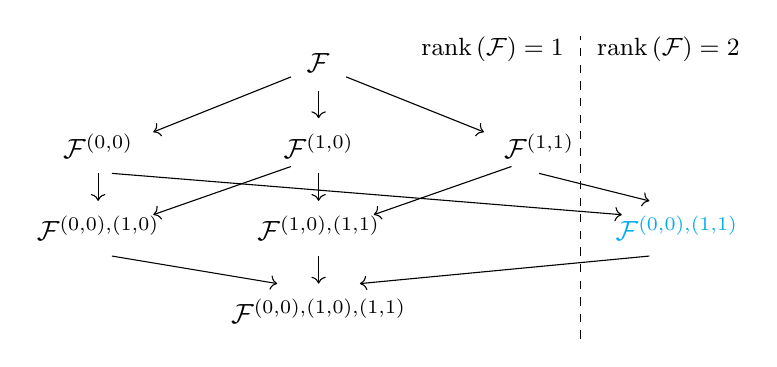
\begin{tikzpicture}[scale=0.35]

    \node[anchor=center] at (0,9) {$\facesymbolof{\varnothing}$};
    \draw[->] (-1,8.5) -- (-6,6.5);
    \draw[->] (0,8) -- (0,7);
    \draw[->] (1,8.5) -- (6,6.5);

    \node[anchor=center] at (-8,6) {$\facesymbolof{(0,0)}$};
    \draw[->] (-8,5) -- (-8,4);

    \node[anchor=center] at (0,6) {$\facesymbolof{(1,0)}$};
    \draw[->] (-1,5.25) -- (-6,3.5);
    \draw[->] (0,5) -- (0,4);

    \node[anchor=center] at (8,6) {$\facesymbolof{(1,1)}$};

    \draw[->] (7,5.25) -- (2,3.5);

    \node[anchor=center] at (-8,3) {$\facesymbolof{(0,0),(1,0)}$};
    \draw[->] (-7.5,2) -- (-1.5,1);
    \node[anchor=center] at (0,3) {$\facesymbolof{(1,0),(1,1)}$};
    \draw[->] (0,2) -- (0,1);

    \node[] (shift) at (5,0) {};
    \draw[->] (8,5) -- ($(7,4)+(shift)$);
    \draw[->] (-7.5,5) -- ($(6,3.5)+(shift)$);
    \node[anchor=center] at ($(8,3)+(shift)$) {\textcolor{\concolor}{$\facesymbolof{(0,0),(1,1)}$}};
    \draw[->] ($(7,2)+(shift)$) -- (1.5,1);

    \draw[dashed] (9.5,-1) -- (9.5,10);
    \node[anchor=west] at (9.75,9.5) {\corelabelsize $\cprankof{\facesymbol}=2$};
    \node[anchor=east] at (9.25,9.5) {\corelabelsize $\cprankof{\facesymbol}=1$};

    \node[anchor=center] at (0,0) {$\facesymbolof{(0,0),(1,0),(1,1)}$};

\end{tikzpicture}
        \end{center}
        \caption{
           Face lattice $\facelatticeof{(\catvariableof{0} \land \catvariableof{1},\catvariableof{0} \Rightarrow \catvariableof{1})}$ to \exaref{exa:nonelHlnstat}.
            The directed arrows represent inclusion of the faces, which is a partial order of the faces.
        The face \textcolor{\concolor}{$\facesymbolof{(0,0),(1,1)}$} is the only face, which is not representable by an elementary hypergraph.
            It is representable in a $\cpformat$ with hidden rank $2$
        }\label{fig:latticeNonelHlnstat}
    \end{figure}

\end{example}

\begin{example}[Atomic formulas]
    \label{exa:atomicFormulasHypercube}
    %The assumption of \theref{the:sufficientHLNExpressivity} is satisfied in
    Let us consider the case of atomic formulas. % where the formulas $\formulaof{\formulaset,\canparam}$ are the atoms.
    The mean polytope in this case is the $\catorder$-dimensional hypercube
    \begin{align*}
        \meansetof{\atomformulaset,\ones} = \fullparcube
    \end{align*}
    which is called a simple polytope, since each vertex is contained in the minimal number of $\catorder$ facets.
    %Since the cube $\fullparcube$ is a face of itself, \theref{the:sufficientHLNExpressivity} implies $\hlnmeanset|_{\hlnsetof{\atomformulaset}}=\hlnmeanset$.

    The faces of a hypercube are enumerated in the following way.
    Each face is characterized by the projections onto each variable, which is either $\{0\}$, $\{1\}$ or $[0,1]$.
    The projections are represented by the tuple $\hardparam$ defined in the following way:
    \begin{itemize}
        \item We define the set $\hardlegset\subset[\atomorder]$ of variables, such that the projection onto the variable is $\{0\}$ or $\{1\}$
        \item We define to each $\selindex\in\hardlegset$ an index $\headindexof{\selindex}=0$ if the projection is $\{0\}$ and $\headindexof{\selindex}=1$ if the projection is $\{1\}$.
    \end{itemize}

%    There are thus $2^{\atomorder}$ different sets $\hardlegset$, each with $2^{\hardlegset}$ faces by a choice of $\headindexof{\selindex}$.

    Trivially, each face of the hypercube is a cube face and $\elmeansetof{\atomformulaset}=\meansetof{\atomformulaset}$.

    \red{More general: If and only if no combination of possibly negated formulas is unsatisfiable, then the mean polytope is a hypercube.}
\end{example}

\begin{example}[Minterm formulas]
    \label{exa:mintermHLNSet}
    The set of minterm formulas is indexed by $\shortcatindicesin$ and given by
    \begin{align*}
        \formulaofat{\shortcatindices}{\shortcatvariables} = \bigwedge_{\selindex\in[\catorder]} \lnot^{1-\catindexof{\selindex}} \formulaofat{\selindex}{\shortcatvariables}
        = \onehotmapofat{\shortcatindices}{\shortcatvariables}
    \end{align*}
    where by $\formulaofat{\selindex}{\shortcatvariables}$ we denote the $\selindex$-th atomic formula (see \exaref{exa:atomicFormulasHypercube}).
    The mean polytope is in the case of the minterm statistic (also referred to as universal statistic) and a boolean base measure $\basemeasure$ the standard simplex of dimension
    \begin{align*}
        \cardof{\shortcatindicesin \wcols \basemeasureat{\indexedshortcatvariables}\neq 0}-1 \, ,
    \end{align*}
    that is the set
    \begin{align*}
        \elmeansetof{\mintermformulaset,\basemeasure}
        = \convhullof{\onehotmapofat{\shortcatindices}{\headvariables}\wcols\shortcatindicesin\ncond\basemeasureat{\indexedshortcatvariables}\neq 0} \, .
    \end{align*}
    In this case, $\hlnsetof{\mintermformulaset}$ contains any distribution and therefore trivially realizes any mean parameter in $\meansetof{\mintermformulaset,\ones}$.

    The faces of the standard simplex are itself standard simplices to base measures $\secbasemeasure$ with $\secbasemeasure\prec\basemeasure$.
    We store them by the tuple $\hardparam$, where $\hardlegset$ is the support of $\secbasemeasure$ and $\headindexof{\selindex}=0$ for $\selindex\in\hardlegset$.
    Each face is a cube face, since it is the intersection of $\hlnsetof{\mintermformulaset}$ with the cube face $\hardparam$.
    In particular, we have $\elmeansetof{\mintermformulaset}=\meansetof{\mintermformulaset}$.

    \red{More general the mean polytope is a standard simplex, if and only if each formula contradicts all others.}
\end{example}

\begin{example}[$\ttformat$ representation of diagonal faces]
    \label{exa:tt_diagonal_face}
    Consider the vertex set
    \begin{align*}
        \imset \coloneqq \{0,1\}^{\seldim} / \imelementat{\selvariable}
    \end{align*}
    convex polytope.
    We are interested in the face $\facesymbolof{\triangleleft,1}$ with the normal $\frac{1}{2} (2\imelementwith - \onesat{\selvariable})$.
    Its vertices are the $\seldim$ elements of $\{0,1\}^{\seldim}$, which differ from $\imelementwith$ in exactly one coordinate (i.e. those with Hamming distance of $1$ from $\imelementat{\selvariable}$).
    We denote these vertices by $\imelementof{\selindex}$ for $\selindexin$, which coordinates to $\secselindex\in[\seldim]$ are
    \begin{align*}
        \imelementofat{\selindex}{\selvariable=\secselindex}
        = \begin{cases}
              \imelementat{\selvariable=\secselindex} & \ifspace \secselindex\neq\selindex \\
              1-\imelementat{\selvariable=\secselindex} & \ifspace \secselindex=\selindex
        \end{cases} \, .
    \end{align*}

    We now represent their sum in an $\ttformat$ with hidden ranks $r_0=\ldots=r_{\seldim-2}=2$.
    The boolean hidden variables are denoted be $\decvariableof{[\seldim-1]}$ and can be interpreted as indicators, whether the coordinate flip has happened in $[\selindex]$ coordinates.
    We now construct a $\ttformat$ cores for $\selindex=0$ by
    \begin{align*}
        \hypercoreofat{0}{\headvariableof{0},\decvariableof{0}}
        = \onehotmapofat{\imelementat{\selvariable=0}}{\headvariableof{0}} \otimes \fbasisat{\decvariableof{0}}
        + \onehotmapofat{1-\imelementat{\selvariable=0}}{\headvariableof{0}} \otimes \tbasisat{\decvariableof{0}}
    \end{align*}
    further for $\selindex\notin\{0,\seldim-1\}$ the cores
    \begin{align*}
        \hypercoreofat{\selindex}{\decvariableof{\selindex-1},\headvariableof{\selindex},\decvariableof{\selindex}}
        = \, & \fbasisat{\decvariableof{\selindex-1}} \otimes \onehotmapofat{1-\imelementat{\indexedselvariable}}{\headvariableof{\selindex}} \otimes \tbasisat{\decvariableof{\selindex}}
        + \fbasisat{\decvariableof{\selindex-1}} \otimes \onehotmapofat{\imelementat{\indexedselvariable}}{\headvariableof{\selindex}} \otimes \fbasisat{\decvariableof{\selindex}} \\
        &+ \tbasisat{\decvariableof{\selindex-1}} \otimes \onehotmapofat{\imelementat{\indexedselvariable}}{\headvariableof{\selindex}} \otimes \tbasisat{\decvariableof{\selindex}}
    \end{align*}
    and for $\selindex=\seldim-1$
    \begin{align*}
        \hypercoreofat{\seldim-1}{\decvariableof{\seldim-1},\headvariableof{\seldim-1}}
        = \fbasisat{\decvariableof{\seldim-1}} \otimes \onehotmapofat{1-\imelementat{\selvariable=\seldim-1}}{\headvariableof{\seldim-1}}
        + \tbasisat{\decvariableof{\seldim-1}} \otimes \onehotmapofat{\imelementat{\selvariable=\seldim-1}}{\headvariableof{\seldim-1}} \, .
    \end{align*}
    For this tensor network in the $\ttformat$ format we have
    \begin{align*}
        \sum_{\selindexin} \onehotmapofat{\imelementof{\selindex}}{\headvariables}
        = \contractionof{\{\hypercoreofat{0}{\headvariableof{0},\decvariableof{0}},\hypercoreofat{\seldim-1}{\decvariableof{\seldim-1},\headvariableof{\seldim-1}}\}\cup\{\hypercoreofat{\selindex}{\decvariableof{\selindex-1},\headvariableof{\selindex},\decvariableof{\selindex}}\wcols\selindex\notin\{0,\seldim-1\}\}}{\headvariables} \, .
    \end{align*}
    The $\ttformat$ multirank of $2$ is furthermore minimal, since each matrification based on a partition of $[\seldim]$ into non-empty sets has a matrix rank of $2$.
    With respect to such partitions also the tensor $\onehotmapofat{\imelement}{\headvariables}+\left(\sum_{\selindexin}\onehotmapofat{\imelementof{\selindex}}{\headvariables}\right)$ has matrix ranks of $2$.
    Since these are the only two activation tensors for the face $\facesymbolof{\triangleleft,1}$.
\end{example}

\begin{example}[Generalization of \exaref{exa:tt_diagonal_face} to larger $\ttformat$ ranks]
    \label{exa:gen_tt_diagonal_face}
    %% Extension to larger Hadamard distances
    We now generalize the construction of \exaref{exa:tt_diagonal_face} by using the Hadamard distance $d(\cdot,\cdot)$ in $\{0,1\}^{\seldim}$, which counts the number of coordinates two vertices differ in.
    For $s\in\{1,\ldots,\seldim-1\}$ we define for a fixed $\imelementwith\in\{0,1\}^{\seldim}$ a polytope as the convex hull
    \begin{align*}
        \{\tilde{\imelement}[\selvariable] \wcols d(\tilde{\imelement},\imelement)\geq s\}  \, .
    \end{align*}
    The face to the normal $\frac{1}{2} (2\imelementwith - \onesat{\selvariable})$ is the convex hull
    \begin{align*}
        \facesymbolof{\triangleleft,s}\coloneqq \convhullof{
            \{\tilde{\imelement}[\selvariable] \wcols d(\tilde{\imelement},\imelement) = s\}
        }
    \end{align*}
    containing $\binom{\seldim}{s}$ vertices.
    We label these vertices by subsets $\variableset\subset[\seldim]$ of cardinality $s$ and define for $\selindexin$
    \begin{align*}
        \imelementofat{\variableset}{\indexedselvariable} =
        \begin{cases}
            \imelementat{\selindexin} & \ifspace \selindex\notin\variableset \\
            1-\imelementat{\selindexin} & \ifspace \selindex\notin\variableset
        \end{cases}
    \end{align*}
    We now construct a $\ttformat$ with hidden variables $\decvariableof{\selindex}$ and ranks $r_{\selindex} = \min (\selindex+1,\seldim-\selindex+1, s+1)$ to represent the sum of their one-hot encodings.
    To this end, let there be $\ttformat$ cores for $\selindex=0$ by
    \begin{align*}
        \hypercoreofat{0}{\headvariableof{0},\decvariableof{0}}
        = \onehotmapofat{\imelementat{\selvariable=0}}{\headvariableof{0}} \otimes \fbasisat{\decvariableof{0}}
        + \onehotmapofat{1-\imelementat{\selvariable=0}}{\headvariableof{0}} \otimes \tbasisat{\decvariableof{0}}
    \end{align*}
    further for $\selindex\notin\{0,\seldim-1\}$ the cores
    \begin{align*}
        \hypercoreofat{\selindex}{\decvariableof{\selindex-1},\headvariableof{\selindex},\decvariableof{\selindex}}
        = \sum_{\selindex\in\{\max(s-\seldim+\selindex,0),\ldots,\max(\selindex,s)\}}
        \onehotmapofat{\selindex}{\decvariableof{\selindex}}
        \otimes \left(\onehotmapofat{\imelementat{\indexedselvariable}}{\headvariableof{\selindex}} \otimes \onehotmapofat{\selindex}{\decvariableof{\selindex+1}}
                    + \onehotmapofat{1-\imelementat{\indexedselvariable}}{\headvariableof{\selindex}} \otimes \onehotmapofat{\selindex+1}{\decvariableof{\selindex+1}}
        \right)
    \end{align*}
    and for $\selindex=\seldim-1$
    \begin{align*}
        \hypercoreofat{\seldim-1}{\decvariableof{\seldim-1},\headvariableof{\seldim-1}}
        = \fbasisat{\decvariableof{\seldim-1}} \otimes \onehotmapofat{1-\imelementat{\selvariable=\seldim-1}}{\headvariableof{\seldim-1}}
        + \tbasisat{\decvariableof{\seldim-1}} \otimes \onehotmapofat{\imelementat{\selvariable=\seldim-1}}{\headvariableof{\seldim-1}} \, .
    \end{align*}
    Based on the interpretation, that the hidden variables $\decvariableof{\selindex}$ count the Hamming distance of the vectors $\restrictionofto{\imelementwith}{\rr^{\selindex}\times 0_{\seldim-\selindex}}$ and the respective $\restrictionofto{\imelementofat{\variableset}{\selvariable}}{\rr^{\selindex}\times 0_{\seldim-\selindex}}$ one can show that
    \begin{align*}
        \sum_{\variableset\subset[\seldim] \wcols \cardof{\variableset}=s} \onehotmapofat{\imelementof{\variableset}}{\headvariables}
        = \contractionof{\{\hypercoreofat{0}{\headvariableof{0},\decvariableof{0}},\hypercoreofat{\seldim-1}{\decvariableof{\seldim-1},\headvariableof{\seldim-1}}\}\cup\{\hypercoreofat{\selindex}{\decvariableof{\selindex-1},\headvariableof{\selindex},\decvariableof{\selindex}}\wcols\selindex\notin\{0,\seldim-1\}\}}{\headvariables} \, .
    \end{align*}
\end{example}

\begin{example}[Generalization of \exaref{exa:gen_tt_diagonal_face} to arbitrary $\htformat$ formats]
    Instead of aligning the Hamming count variables linearly, one can find a representation of the activation tensor
    \begin{align*}
        \sum_{\variableset\subset[\seldim] \wcols \cardof{\variableset}=s} \onehotmapofat{\imelementof{\variableset}}{\headvariables}
    \end{align*}
    in an arbitrary directed acyclic tree hypergraph format $\graph$, which hidden ranks are bounded by the number of leafs in the subtree and $s+1$.

    At any leaf of the tree we define a $2x2$ matrix
    \begin{align*}
        \hypercoreofat{\selindex}{\headvariableof{\selindex},\decvariableof{\selindex}}
        = \onehotmapofat{\imelementat{\indexedselvariable}}{\headvariableof{\selindex}} \otimes \fbasisat{\decvariableof{\selindex}}
        + \onehotmapofat{1-\imelementat{\indexedselvariable}}{\headvariableof{\selindex}} \otimes \tbasisat{\decvariableof{\selindex}} \, .
    \end{align*}
    At each intermediate non-root hyperedge we choose an outgoing counting variable $\decvariableof{\outgoingnodes}$ with dimension by $\decdimof{\outgoingnodes}=\min(\sum_{\node\in\incomingnodes}\decdimof{\incomingnodes},s+1)$ and define a tensor with the slices
    \begin{align*}
        \hypercoreofat{\edge}{\decvariableof{\outgoingnodes},\decvariableof{\incomingnodes}}
        = \bencodingofat{+}{\headvariableof{+}=\decindexof{\outgoingnodes},\decvariableof{\incomingnodes}} \, .
    \end{align*}
    We further build at the root hyperedge $\edge$ a tensor
    \begin{align*}
        \hypercoreofat{\edge}{\decvariableof{\edge}}
        = \sum_{\decindex \wcols \contraction{\decindex}=s}
        \onehotmapofat{\decindexof{\edge}}{\decvariableof{\edge}} \, .
    \end{align*}
    Using the counting variable interpretation one can now show that
    \begin{align*}
        \sum_{\variableset\subset[\seldim] \wcols \cardof{\variableset}=s} \onehotmapofat{\imelementof{\variableset}}{\headvariables}
        =\contractionof{
        \{\hypercoreofat{\edge}{\decvariableof{\edge}} \wcols \edgein \} \cup \{\hypercoreofat{\selindex}{\headvariableof{\selindex},\decvariableof{\selindex}} \wcols \nodein\}
        }{\headvariables} \, .
    \end{align*}
\end{example}

\subsection{Construction of \HybridLogicNetworks{}}

We now constructively show, that any convex polytope with boolean vertices in $\parspace$ (a so called 0-1 polytope, see \cite{ziegler_lectures_2000}) is the mean polytope of a family of \HybridLogicNetworks{}.

\begin{theorem}
    Let $\meanset$ an arbitrary polytope with boolean vertices in $\parspace$.
    Then we construct propositional formulas on atoms $\catvariableof{[\seldim]}$ by
    \begin{align*}
        \formulaofat{0}{\catvariableof{0}} =
        \begin{cases}
            \top & \ifspace \restrictionofto{\meanset}{\rr^1\times 0_{\seldim-1}} = \{1\} \\
            \bot & \ifspace \restrictionofto{\meanset}{\rr^1 \times 0_{\seldim-1}} = \{0\} \\
            \catvariableof{0} & \ifspace \restrictionofto{\meanset}{\rr^1 \times 0_{\seldim-1}} = [0,1]
        \end{cases}
    \end{align*}
    and iteratively for $\selindexin$ with $\selindex\geq1$ by
    \begin{align*}
        \formulaofat{\selindex}{\catvariableof{[\selindex+1]}} =
        \bigwedge_{v[\selvariable] \in \restrictionofto{\meanset}{\rr^\selindex\times 0_{\seldim-\selindex}}\cap \{0,1\}^{\seldim}}
        \left(\left(\bigwedge_{\secselindex\in[\selindex+1]} \lnot^{1-v[\indexedselvariable]} \formulaofat{\selindex}{\catvariableof{[\selindex]}}\right) \Rightarrow
            \begin{cases}
                \top & \ifspace \restrictionofto{\meanset}{v\times\rr^{1} \times 0_{\seldim-\selindex-1}} = \{1\} \\
                \bot & \ifspace \restrictionofto{\meanset}{v\times\rr^{1} \times 0_{\seldim-\selindex-1}} = \{0\} \\
                \catvariableof{\selindex} & \ifspace \restrictionofto{\meanset}{v\times\rr^{1} \times 0_{\seldim-\selindex-1}} = \{0,1\} \\
            \end{cases}
        \right).
    \end{align*}
    Here we denote by $\restrictionofto{\meanset}{V}$ the projections of the vertices in $\meanset$ onto the subspaces $V$, and by $0_{\seldim}$ the zero vector in $\rr^{\seldim}$.
\end{theorem}
\begin{proof}
    We show per induction, that for any $\selindexin$ the family of \HybridLogicNetworks{} with the statistic $\formulaof{[\selindex+1]}$ by the first $\selindex+1$ formulas has the mean polytope
    \begin{align}
        \label{eq:HLNindConTBS}
        \meansetof{\formulaof{[\selindex+1]},\trivbm} = \restrictionofto{\meanset}{\rr^\selindex\times 0_{\seldim-\selindex}} \, .
    \end{align}

    $\selindex=0$: The polytope $\restrictionofto{\meanset}{\rr^\selindex\times 0_{\seldim-\selindex}}=\{1\}$ (respectively $\restrictionofto{\meanset}{\rr^\selindex\times 0_{\seldim-\selindex}}=\{0\}$) is reproduced by $\formulaof{0}$ being a tautology (respectively a contradiction).
    In the case $\restrictionofto{\meanset}{\rr^\selindex\times 0_{\seldim-\selindex}}=[0,1]$ the polytope is reproduced by the any formula, which is neither a tautology nor a contradiction, and the atomic formula $\catvariableof{0}$ is an example of such an contingency.
    Since the projection of a 0-1 polytope onto the first coordinates is itself a 0-1 polytope, these are the only possible cases and we conclude that in all
    \begin{align*}
        \meansetof{\formulaof{[\selindex+1]},\trivbm} = \restrictionofto{\meanset}{\rr^\selindex\times 0_{\seldim-\selindex}} \, .
    \end{align*}

    $\selindex\rightarrow\selindex+1$: Let us assume, that \eqref{eq:HLNindConTBS} holds for a $\selindexin$.
    Then for any $\shortcatindicesin$ there is exactly one $v[\selvariable] \in \restrictionofto{\meanset}{\rr^\selindex\times 0_{\seldim-\selindex}}$ such that $\shortcatindices$ is a model of
    \begin{align*}
        \formulaof{\selindex,v}\coloneqq
        \bigwedge_{\secselindex\in[\selindex+1]} \lnot^{1-v[\indexedselvariable]} \formulaofat{\selindex}{\catvariableof{[\selindex]}} \, .
    \end{align*}
    This holds, since by the mutual contradiction of these formulas at most one can have $\shortcatindices$ as a model.
    Further, if none would have $\shortcatindices$ as a model, then the to $\shortcatindices$ corresponding vector of satisfactions $(\formulaofat{\selindex}{\indexedshortcatvariables})_{\selindex\in[\selindex]}$ is not in $\restrictionofto{\meanset}{\rr^\selindex\times 0_{\seldim-\selindex}}$, which can not be the case.
    Now, the implications to all $\tilde{v}$ except for $v$ are for the models $\shortcatindices$ of $\formulaof{\selindex,v}$ satisfied, and the satisfaction of $\formulaof{\selindex}$ thus only depends on the head of the implication to $v$.
    It follows, that the vertices of $\meansetof{\formulaof{[\selindex+2]},\trivbm}$ sharing the first $\selindex$ coordinates with $v$ are determined by the head of the implication at $v$.
    With the same arguments as in the case $\selindex=0$ we now notice, that in the three cases we construct vertex sets $v\times\{1\},\, v\times\{1\}$ or $v\times\{0,1\}$ if and only if they appear in the polytope $\restrictionofto{\meanset}{\rr^{\selindex+1}\times 0_{\seldim-\selindex-1}}$.
    This establishes for each vertex $v$ of $\meansetof{\formulaof{[\selindex+1]},\trivbm}$ that
    \begin{align*}
        \restrictionofto{\left(\meansetof{\formulaof{[\selindex+2]},\trivbm}\right)}{v\times\rr\times0_{\seldim-\selindex-1}}
        = \restrictionofto{\left(\restrictionofto{\meanset}{\rr^\selindex\times 0_{\seldim-\selindex}}\right)}{v\times\rr\times0_{\seldim-\selindex-1}} \, .
    \end{align*}
    Since for any vertex in $\meanset$ we find a unique vertex in $\meansetof{\formulaof{[\selindex+1]},\trivbm}$ sharing the first $\selindex$ coordinates, we have that \eqref{eq:HLNindConTBS} holds for $\selindex+1$.

    By induction the equation \eqref{eq:HLNindConTBS} holds for arbitrary $\selindexin$.
    For $\selindex=\seldim-1$ the equation is the claim.
\end{proof}

\subsection{Further Examples of non-cubelike polytopes}

\begin{example}[Ising model on $2$ nodes]
    % See Example~3.6 in \cite{wainwright_graphical_2008}
    Consider two boolean variables $\catvariableof{0},\catvariableof{1}$ and the Ising statistic by three propositional formulas
    \begin{align*}
        \formulaofat{0}{\catvariableof{[2]}} = \catvariableof{0} \quad , \quad
        \formulaofat{1}{\catvariableof{[2]}} = \catvariableof{1} \andspace
        \formulaofat{2}{\catvariableof{[2]}} = \catvariableof{0}\land\catvariableof{1} \, .
    \end{align*}
    In the Ising interpretation, the boolean variables represent interacting spins at two locations.
    Their value is then measured by the first two formulas and their interaction by the third.

    The vertices of the mean polytope to this statistic are
    \begin{align*}
        \hlnstatat{\catindexof{0},\catindexof{1}} = [\formulaofat{0}{\indexedcatvariableof{[2]}},\formulaofat{1}{\indexedcatvariableof{[2]}},\formulaofat{2}{\indexedcatvariableof{[2]}}]^T =
        \begin{cases}
        [0,0,0]
            ^T & \ifspace (\catindexof{0},\catindexof{1}) = (0,0) \\
            [0,1,0]^T & \ifspace (\catindexof{0},\catindexof{1}) = (0,1) \\
            [1,0,0]^T & \ifspace (\catindexof{0},\catindexof{1}) = (1,0) \\
            [1,1,1]^T & \ifspace (\catindexof{0},\catindexof{1}) = (1,1)
        \end{cases}
    \end{align*}
    and the mean polytope is the convex hull of these, sketched as:
    \begin{center}
        \tdplotsetmaincoords{55}{20} % Set the viewpoint: (theta, phi)

        \begin{tikzpicture}[tdplot_main_coords, scale=2,
            mainline/.style={thick},
            invisibleline/.style={dashed, gray}
        ]

            % Define the 4 vertices
            \coordinate (A) at (0, 0, 0);
            \coordinate (B) at (0, 1, 0);
            \coordinate (C) at (1, 0, 0);
            \coordinate (D) at (1, 1, 1);

            % Draw the faces with some opacity (optional, requires more complex sorting for correct rendering)
            \fill[cyan!20, opacity=0.6] (A) -- (B) -- (C) -- cycle;
            % \fill[cyan!20, opacity=0.6] (A) -- (B) -- (D) -- cycle;
            % \fill[cyan!20, opacity=0.6] (A) -- (C) -- (D) -- cycle;
            % \fill[cyan!20, opacity=0.6] (B) -- (C) -- (D) -- cycle;

            % Draw visible edges (adjust based on your chosen viewpoint)
            \draw[mainline] (B) -- (C) -- (D) -- cycle; % Front face BCD
            \draw[mainline] (A) -- (B);
            \draw[mainline] (A) -- (C);
            \draw[mainline] (A) -- (D);

            % Draw the hidden edge (adjust based on your chosen viewpoint)
            % In this view, edge BC is visible, but the edge connecting the back vertex to D is also potentially visible.
            % The edge BC is visible, the edge connecting A to C and B is also visible.
            % A is behind for this viewpoint, so the edges connected to A are back edges
            \draw[invisibleline] (A) -- (B);
            \draw[invisibleline] (A) -- (C);
            \draw[invisibleline] (A) -- (D);


            % Draw vertices as nodes and label them
            \foreach \point/\label/\pos in {A/000/below left, B/010/below right, C/100/above left, D/111/above} {
                \draw[fill=black] (\point) circle (1pt) node[\pos] {$\label$};
            }

            % Add coordinate system axes for context
            \draw[->, gray] (0,0,0) -- (1.2,0,0) node[right] {$\meanparamat{\selvariable=0}$};
            \draw[->, gray] (0,0,0) -- (0,1.2,0) node[above] {$\meanparamat{\selvariable=1}$};
            \draw[->, gray] (0,0,0) -- (0,0,1.2) node[above] {$\meanparamat{\selvariable=2}$};

        \end{tikzpicture}
    \end{center}

    We notice, that the convex hull of any three out of the four vertices builds a facet.
    The only cube-like facet of these four is the convex hull of $\{[0,0,0]^T,[1,0,0]^T,[0,1,0]\}$ (sketched in cyan in the above plot) to which we have the parametrization by $(\hardlegset,\headindexof{\hardlegset})=(\{2\},0)$.

    As a consequence, there are maximum entropy distributions of mean parameters in the Ising statistics, which do not have a representation by an elementary \CompActNet{} in the Ising statistic.
\end{example}

\begin{example}[Crossword Polytopes]
    % See Example~3.9 in \cite{wainwright_graphical_2008}
    Consider the crossword polytope with the vertices
    \begin{align*}
        \{\headindexof{[3]} \wcols \sum_{\catenumerator\in[3]} \headindexof{\catenumerator}=0 \}
    \end{align*}
    We interpret the vertices by the strings of length $3$, which parity vanishes.
    Such constrained are common in the construction of codewords using parity-check codes (see \cite{gallager_low-density_1963}).
    \begin{center}
        \tdplotsetmaincoords{55}{30} % Set the viewpoint: (theta, phi)

        \begin{tikzpicture}[tdplot_main_coords, scale=2,
            mainline/.style={thick},
            invisibleline/.style={dashed, gray}
        ]

            % Define the 4 vertices
            \coordinate (A) at (0, 0, 0);
            \coordinate (B) at (0, 1, 1);
            \coordinate (C) at (1, 0, 1);
            \coordinate (D) at (1, 1, 0);

            % Draw the faces with some opacity (optional, requires more complex sorting for correct rendering)
            %\fill[cyan!20, opacity=0.6] (A) -- (B) -- (C) -- cycle;
            % \fill[cyan!20, opacity=0.6] (A) -- (B) -- (D) -- cycle;
            % \fill[cyan!20, opacity=0.6] (A) -- (C) -- (D) -- cycle;
            % \fill[cyan!20, opacity=0.6] (B) -- (C) -- (D) -- cycle;

            % Draw visible edges (adjust based on your chosen viewpoint)
            \draw[mainline] (B) -- (C) -- (D) -- cycle; % Front face BCD
            \draw[mainline] (A) -- (B);
            \draw[mainline] (A) -- (C);
            \draw[mainline] (A) -- (D);

            % Draw the hidden edge (adjust based on your chosen viewpoint)
            % In this view, edge BC is visible, but the edge connecting the back vertex to D is also potentially visible.
            % The edge BC is visible, the edge connecting A to C and B is also visible.
            % A is behind for this viewpoint, so the edges connected to A are back edges
            \draw[invisibleline] (A) -- (B);
            \draw[invisibleline] (A) -- (C);
            \draw[invisibleline] (A) -- (D);


            % Draw vertices as nodes and label them
            \foreach \point/\label/\pos in {A/000/below left, B/011/below right, C/101/above left, D/110/above} {
                \draw[fill=black] (\point) circle (1pt) node[\pos] {$\label$};
            }

            % Add coordinate system axes for context
            \draw[->, gray] (0,0,0) -- (1.2,0,0) node[right] {$\meanparamat{\selvariable=0}$};
            \draw[->, gray] (0,0,0) -- (0,1.2,0) node[above] {$\meanparamat{\selvariable=1}$};
            \draw[->, gray] (0,0,0) -- (0,0,1.2) node[above] {$\meanparamat{\selvariable=2}$};

        \end{tikzpicture}
    \end{center}

    All facets are non-cube-like, whereas all other faces are cube-like (the edges are labeled by the $6$ facets of $[0,1]^3$).

    %% Hamming distance characterization and TT characterization
    Each facet is characterized by the Hamming distance of exactly $1$ to a single of the $4$ cube vertices, which are not codewords (see Example~3.9 in \cite{wainwright_graphical_2008}).
    We can construct $\ttformat$ activation tensors with rank $2$, which are calculating in the hidden ranks the Hamming distance to these vertex.
    Each core tensor in that format adds the contribution of a mode to the Hamming distance.

    %% LDPC in more generality: Cycle Polytopes
    In more generality, Low-Density-Parity-Checking Codes (see \cite{gallager_low-density_1963}) construct codewords by a collection of parity constraints on subsets of variables.
    Such polytopes are also known as cycle polytopes, and studied e.g. in \cite{grotschel_geometric_1993}.

\end{example}

    \section{Mean as a Statistic}

We in this section take the perspective of estimating a maximum entropy distribution given observed data.
\begin{itemize}
    \item $\datamean$ is an unbiased estimator of $\meanparam$, i.e. $\expectationof{\datameanat{\selvariable}}=\meanparam$
    \item $\datamean$ is a consistent estimator of $\meanparam$, i.e. $\datameanat{\selvariable}\rightarrow\meanparam$ by the law of large numbers coordinatewise almost everywhere.
    \item $\datamean$ is the minimal variance unbiased estimator of $\meanparam$. %CHECK
\end{itemize}


The mean parameter $\datamean$ given a dataset can be understood as a statistic of the dataset.
We here show that for the family of maximum entropy distributions this statistic is a minimal sufficient statistic.

The family of maximum entropy distributions is the set
\begin{align*}
    \left\{ \probofat{\meanparam}{\shortcatvariables} \wcols \meanparam\in\meansetof{\sstat,\basemeasure}\right\}
\end{align*}
which has been characterized above by a union of exponential families with respect to face measures.

Taking a frequentist perspective we now understand datasets by random variables $\catvariableof{[\catorder]\times[\datanum]}$, where for $\datindexin$ the variables $\catvariableof{[\catorder],\datindex}$ are drawn i.i.d. from a maximum entropy distribution.
The mean statistic is then a tensor
\begin{align*}
    \datameanat{\catvariableof{[\catorder]\times[\datanum]},\selvariable}
\end{align*}
whith coordinates
\begin{align*}
    \datameanat{\indexedcatvariableof{[\catorder]\times[\datanum]},\selvariable}
    = \frac{1}{\datanum}\sum_{\datindexin} \sencodingofat{\sstat}{\indexedcatvariableof{[\catorder],\datindex},\selvariable} \, .
\end{align*}


\begin{theorem}
    The mean statistic is a sufficient statistic for the family of maximum entropy distributions $(\sstat,\basemeasure)$.
    If the base measure has maximal support, the mean statistic is in addition minimal.
\end{theorem}
\begin{proof}
    It sufficies to show that the likelihood is a function of $\datamean$.
    Let us choose a face $\facecondset$ of $\genmeanset$, then the likelihood is different from $0$ if and only if the empirical distribution is representable with respect to the face measure.
    This is the case if and only if $\datamean$ is on the face.
    In case that $\datamean$ is on the face, then the likelihood of any distribution on that face exponential family is
    \begin{align*}
        \expof{\datanum\cdot \left(\contraction{\datameanat{\catvariableof{[\catorder]\times[\datanum]},\selvariable},\canparamwith} - \cumfunctionof{\canparam}\right)}
    \end{align*}
    We have thus shown that the likelihood is always a function of $\datamean$.

    The minimality claim can be shown by the constant quotient criterion (see Thm. 6.2.13 in \cite{casella_statistical_2001}).
\end{proof}

    \section{Outlook}

This is relevant for Parameter Estimation: Instabilities when fitting a mean parameter on a non cube-like face.

Further theory to be investigated:
\begin{itemize}
    \item Face representability of randomly drawn polytopes (e.g. expectation of a face rank).
    \item Asymptotic properties for large polytopes (does the average face rank concentrate at an expectation)?
\end{itemize}

Investigate the connection with convex polytope investigations:
\begin{itemize}
    \item Facet complexity (the amount of information to specify the face by inequalities) \cite{grotschel_geometric_1993}
\end{itemize}

Border-rank development to resolve the issue of non-elementary faces:
When defining a boarder rank of the activation tensors by limiting \CompActNets{}, then any maximum entropy distribution has border rank 1.

Application in NeSy:
By format selection (i.e. which complexity is required to represent a face).

    \bibliographystyle{plainnat}
    \bibliography{../../references.bib}

    \appendix

    \section{TT Face Activation}

\subsection{Generic Construction}

When the vertices are characterized by the sum of local terms, we can construct the face activation tensor in $\ttformat$ format, by summation cores.
This is for example the case for the examples constructed based on Hamming distances.

\subsection{Relation with Facet Complexity}

Facet complexity \cite[Definition 6.2.2]{grotschel_geometric_1993} bounds the encoding length of the inequalities describing a polytope.

For any face $\facesymbol$ we find a normal $\normalvec\in\parspace$ and $\normalbound\in\rr$ such that $x$
\begin{align*}
    \genfaceset =
    \{\meanparamwith\in\meanset \wcols \contraction{\normalvecwith,\meanparamwith}=\normalbound \}\, .
\end{align*}
We can thus represent a face activating tensor by computing the contraction $\contraction{\normalvecwith,\headindex[\selvariable]}$.

To this end, let $\arbset\subset\rr$ be a set with index interpretation function
\begin{align*}
    \indexinterpretation : [r] \rightarrow \arbset \, .
\end{align*}
We demand $0,\normalbound\in\arbset$.
We can for example choose $\arbset$ as the $\catorder$-bit binary integer representation.

We then define for $\selindexin$ the summation operations
\begin{align*}
    +^{\selindex,\normalvecat{\indexedselvariable}} \defcols \arbset \times [\headdim] \rightarrow \arbset
\end{align*}
which satisfies for any $\arbelementin$ and $\headindexof{\selindex}$ for which $\arbelement + \normalvecat{\indexedselvariable} \cdot \headindexof{\selindex}\in\arbset$ the equation
\begin{align*}
    +^{\selindex,\normalvecat{\indexedselvariable}}(\arbelement,\headindexof{\selindex})
    = \arbelement + \normalvecat{\indexedselvariable} \cdot \headindexof{\selindex} \, .
\end{align*}
We further assume, that for any tuple $\headindexof{[\seldim]}\in\headstates$ and any $\secselindex\in[\seldim]$
\begin{align*}
    \sum_{\selindex\leq\secselindex} \normalvecat{\indexedselvariable} \cdot \headindexof{\secselindex} \in \arbset \, .
\end{align*}

%Note that we might also use an approximation scheme of the sum on $\arbset$.


Then we have
\begin{align*}
    \sum_{\meanparam\in\genfaceimset} \onehotmapofat{\meanparam}{\headvariables}
    = \contractionof{\{
        \bencodingofat{+^{\selindex,\normalvecat{\indexedselvariable}}}{
            \headvariableof{+^{\selindex,\normalvecat{\indexedselvariable}}},\headvariableof{\selindex}
        }
        \wcols\selindexin\}
        \cup \{\onehotmapofat{\invindexinterpretationat{0}}{\headvariableof{+^{-1,\normalvecat{\selvariable=-1}}}},
        \onehotmapofat{\invindexinterpretationat{\normalbound}}{\headvariableof{+^{\seldim-1,\normalvecat{\selvariable=\seldim-1}}}}\}
    }{\headvariables} \, .
\end{align*}
The variable $\headvariableof{+^{-1,\normalvecat{\selvariable=-1}}}$ is auxiliary to initialize the sum with $0$.

We can weaken the assumptions on $\arbset$:
When $\normalvecwith$ is positive, then any partial sum which exceeds $\normalbound$ can be represented by any member of $\arbset$ which is larger than $\normalbound$.
This brings further sparsity, since no values larger than $\normalbound$ are needed to represent the face (add for example the $\infty$ element to $\arbset$ and represent any partial sum exceeding $\normalbound$ by it).


\begin{definition}
    We say that a face $\facesymbol$ has \emph{TT face complexity} $r$ if there exists a normal $\normalvec\in\parspace$ and $\normalbound\in\rr$ with
    \begin{align*}
        \genfaceset =
        \{\meanparamwith\in\meanset \wcols \contraction{\normalvecwith,\meanparamwith}=\normalbound \}\, .
    \end{align*}
    and there is a subset $\arbset$ of cardinality at most $r$, for which $0,\normalbound\in\arbset$ and for any tuple $\headindexof{[\seldim]}\in\headstates$ and any $\secselindex\in[\seldim]$
    \begin{align*}
        \sum_{\selindex\leq\secselindex} \normalvecat{\indexedselvariable} \cdot \headindexof{\secselindex} \in \arbset \, .
    \end{align*}
\end{definition}

Comparison with facet complexity \cite[Definition 6.2.2]{grotschel_geometric_1993}:
\begin{itemize}
    \item We define complexity here without the log (which would get the string length), to make a direct connection with TT ranks.
    \item Facet complexity considers only the representation of the equation, not the demand of computing it.
    \item Facet complexity considers just facets, not general faces, since it makes a statement about encoding the halfspace representation of the whole polytope.
\end{itemize}

\begin{theorem}
    Let $\facesymbol$ be a face with TT face complexity $r$.
    Then the face activation tensor has a $\ttformat$ rank of at most $r$.
\end{theorem}
\begin{proof}
    See above construction.
\end{proof}



\end{document}